\documentclass[UTF8,12pt]{article}
\usepackage{ctex}
\usepackage{indentfirst}
\usepackage{color}
\usepackage{hyperref}
\usepackage{graphicx}
\usepackage{subfigure}
\usepackage{pdfpages}
\usepackage{listings}
\usepackage{afterpage}
\usepackage{geometry}

\geometry{a4paper,scale=0.8}

\newcommand\myemptypage{
    \null
    \thispagestyle{empty}
    \addtocounter{page}{-1}
    \newpage
}

\hypersetup{
    hidelinks,
	colorlinks=true,
	allcolors=black,
	pdfstartview=Fit,
	breaklinks=true
}

\definecolor{dkgreen}{rgb}{0,0.6,0}
\definecolor{gray}{rgb}{0.5,0.5,0.5}
\definecolor{mauve}{rgb}{0.58,0,0.82}

\lstset{ %
  language=Octave,                % the language of the code
  basicstyle=\footnotesize,           % the size of the fonts that are used for the code
  numbers=left,                   % where to put the line-numbers
  numberstyle=\tiny\color{gray},  % the style that is used for the line-numbers
  stepnumber=2,                   % the step between two line-numbers. If it's 1, each line 
                                  % will be numbered
  numbersep=5pt,                  % how far the line-numbers are from the code
  backgroundcolor=\color{white},      % choose the background color. You must add \usepackage{color}
  showspaces=false,               % show spaces adding particular underscores
  showstringspaces=false,         % underline spaces within strings
  showtabs=false,                 % show tabs within strings adding particular underscores
  frame=single,                   % adds a frame around the code
  rulecolor=\color{black},        % if not set, the frame-color may be changed on line-breaks within not-black text (e.g. commens (green here))
  tabsize=2,                      % sets default tabsize to 2 spaces
  captionpos=b,                   % sets the caption-position to bottom
  breaklines=true,                % sets automatic line breaking
  breakatwhitespace=false,        % sets if automatic breaks should only happen at whitespace
  title=\lstname,                   % show the filename of files included with \lstinputlisting;
                                  % also try caption instead of title
  keywordstyle=\color{blue},          % keyword style
  commentstyle=\color{dkgreen},       % comment style
  stringstyle=\color{mauve},         % string literal style
  escapeinside={\%*}{*)},            % if you want to add LaTeX within your code
  morekeywords={*,...}               % if you want to add more keywords to the set
}


\setlength{\parindent}{2em}

\begin{document}

\begin{titlepage}
    \includepdf[pages={1}]{cover.pdf}
\end{titlepage}

\myemptypage

\begin{center}
    \tableofcontents
\end{center}

\newpage

\section{问题描述}
\subsection{实践目的}
通过指导学生上机实践,让学生学会综合运用所学过的《计算机程序设计基础》、《数据结构》、《算法》、《Java语言与系统设计》、《数据库》、《Web技术》、《移动应用开发》等课程的基础知识,从而能够熟练掌握开发市面上比较流行的移动应用开发的基本技能,设计和开发出具有一定规模的Android客户端应用+JSP(PHP)服务器端编程+MySQL数据库的典型移动互联网应用。

\subsection{课程设计的基本要求}
\begin{itemize}
    \item 知识:了解HTML、HTML5、CSS、JavaScript、JSP、Android等开发技术在实际移动互联网应用开发过程中的基本用法;
    了解移动互联网应用开发从需求分析、系统设计、模块设计、开发以及调试的各个环节。
    掌握典型移动互联网应用各个环节的技术以及具体运用方式;
    了解移动互联网典型应用开发是如何结合Web相关技术(HTML、HTML5、CSS、JavaScript、JSP等)、移动客户端开发技术(Android为例)以及数据库技术(以MySQL为例)进行开发的。
    \item 能力:通过从无到有动手完成基于Web+Android+MySQL移动应用开发的案例的设计、编码和调试工作,将对移动互联网应用开发的理性认识转变为感性认识,
    初步体会和理解计算机相关学科的软件项目工程的具体概念,体会工程的复杂性;学会将理论知识与实际生产结合,学会用工程的角度去提出问题、分析问题和解决问题;
    初步建立移动互联网应用软件工程开发项目需求分析、总体设计、模块设计、编码实现和调试的完整概念,提高实际动手能力,
    为具备大型移动互联网应用开发软件系统从设计到开发的能力打下坚实基础。
    \item 素质:通过实际动手设计和开发多个完整的移动互联网应用实例,培养理论知识的综合运用能力和动手编程开发的能力,培养软件工程开发的流程化管理观念;在实习中理解并遵守软件工程开发的职业道德和规范,履行责任,提高职业规范素质。
\end{itemize}

\subsection{项目基本内容与要求}
\begin{enumerate}
    \item 用Android开发看病预约客户端
    \item 用JSP或PHP开发预约挂号Web服务器
    \item 用MySQL做预约挂号Web服务器的后台数据库
    \item 可以预约挂号、查看医生介绍及日程安排列表等功能
    \item 可以实现患者注册、登录功能
    \item 在线挂号支付
\end{enumerate}

\section{需求分析}
\subsection{开发环境}
\begin{itemize}
    \item 数据库
    \\集成环境:Navicat Premium 16
    \\MySQL 5.7.31
    \item Web服务器
    \\集成环境:Intellij IDEA 2023.1.4
    \\JDK 17.0.4.1
    \\Tomcat 9.0.55
    \\Servlet
    \item Android客户端
    \\集成环境:Android Studio 2022.3.1
    \\Android SDK 31.0.0
    \item 后台管理系统
    \\JSP
    \\LayUI
\end{itemize}

\subsection{用例分析}
本应用作为医院的看病预约应用

主要的actor是患者


主要的use case包括以下几个:
\begin{itemize}
    \item 患者注册
    \item 患者登录
    \item 患者预约挂号
    \begin{itemize}
        \item 患者选择科室
        \item 患者选择医生
        \item 患者选择预约时间
        \item 患者在线支付
        \item 患者查看医生介绍
    \end{itemize}
    \item 患者查看自己的预约挂号
\end{itemize}

\begin{figure}[htbp]
    \centering
    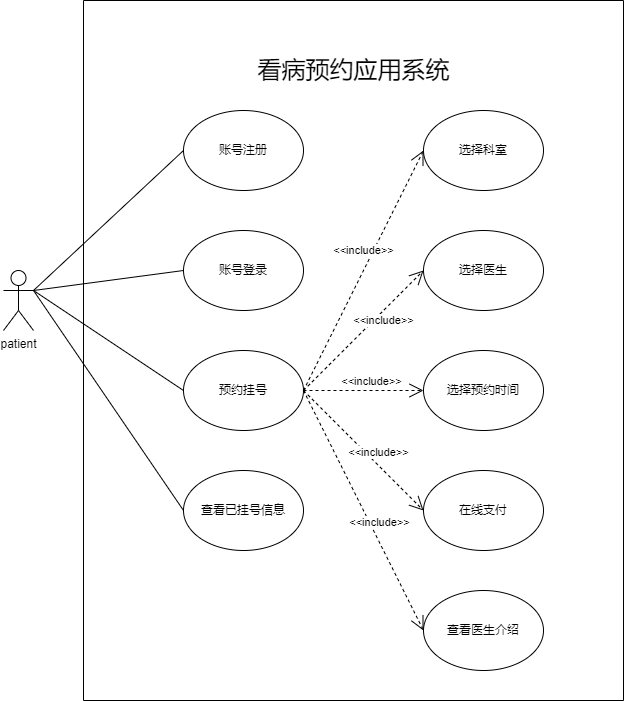
\includegraphics[width=0.9\textwidth]{imgs/1.png}
    \caption{看病预约应用用例图}
\end{figure}

\newpage

\section{设计思想}
设计采用前后端分离的思想,即前端使用Android客户端,后端使用Tomcat服务器,后台管理系统使用layui编写,数据持久化使用MySQL分表存储所有数据。

前端只负责与用户进行交互,后端负责处理用户的请求、验证并返回数据,同时后端负责对数据库的操作,包括表中记录的增删查改。前端不存储数据,减少了用户端的存储空间,减少了用户端的开发难度,同时保证了数据的安全性。

\begin{figure}[htbp]
    \centering
    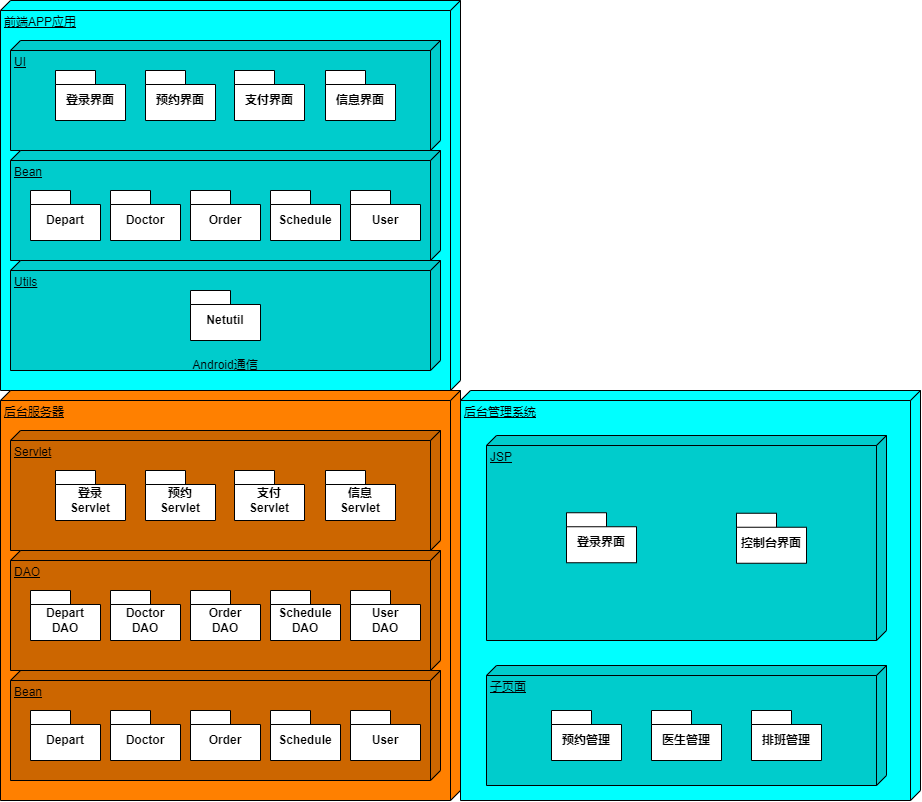
\includegraphics[width=1.0\textwidth]{imgs/15.png}
    \caption{前后端分离架构图}
\end{figure}

\newpage

\section{概要设计}

\subsection{数据库概要设计}
新建数据库并命名为hospital,数据库的结构如下

\begin{lstlisting}[frame=shadowbox]
+--------------------+
| Tables_in_hospital |
+--------------------+
| administrator      |
| depart             |
| doctor             |
| myorder            |
| schedule           |
| user               |
+--------------------+
\end{lstlisting}

六个表中的作用如下:

\begin{itemize}
    \item user表:存储用户相关信息
    \item depart表:存储科室相关信息
    \item doctor表:存储医生相关信息
    \item schedule表:存储医生的排班信息
    \item myorder表:存储用户的预约挂号信息
    \item admistrator表:存储管理员信息
\end{itemize}

\subsection{Android看病预约客户端概要设计}
包括以下几个界面:
\begin{itemize}
    \item 启动界面
    \item 登录界面
    \item 注册界面
    \item 用户首页
    \item 科室列表
    \item 医生列表
    \item 排班时间选择
    \item 我的预约
\end{itemize}

\subsection{后台管理系统概要设计}
包括以下几个界面:
\begin{itemize}
    \item 登录界面
    \item 注册界面
    \item 医生管理
    \item 排班管理
    \item 预约管理
\end{itemize}

\newpage

\section{详细设计}

\subsection{数据库详细设计}

\subsubsection{user表}
user表的主要字段有uid,uname,upsw,分别代表用户id,用户名,密码

\begin{figure}[htbp]
    \centering
    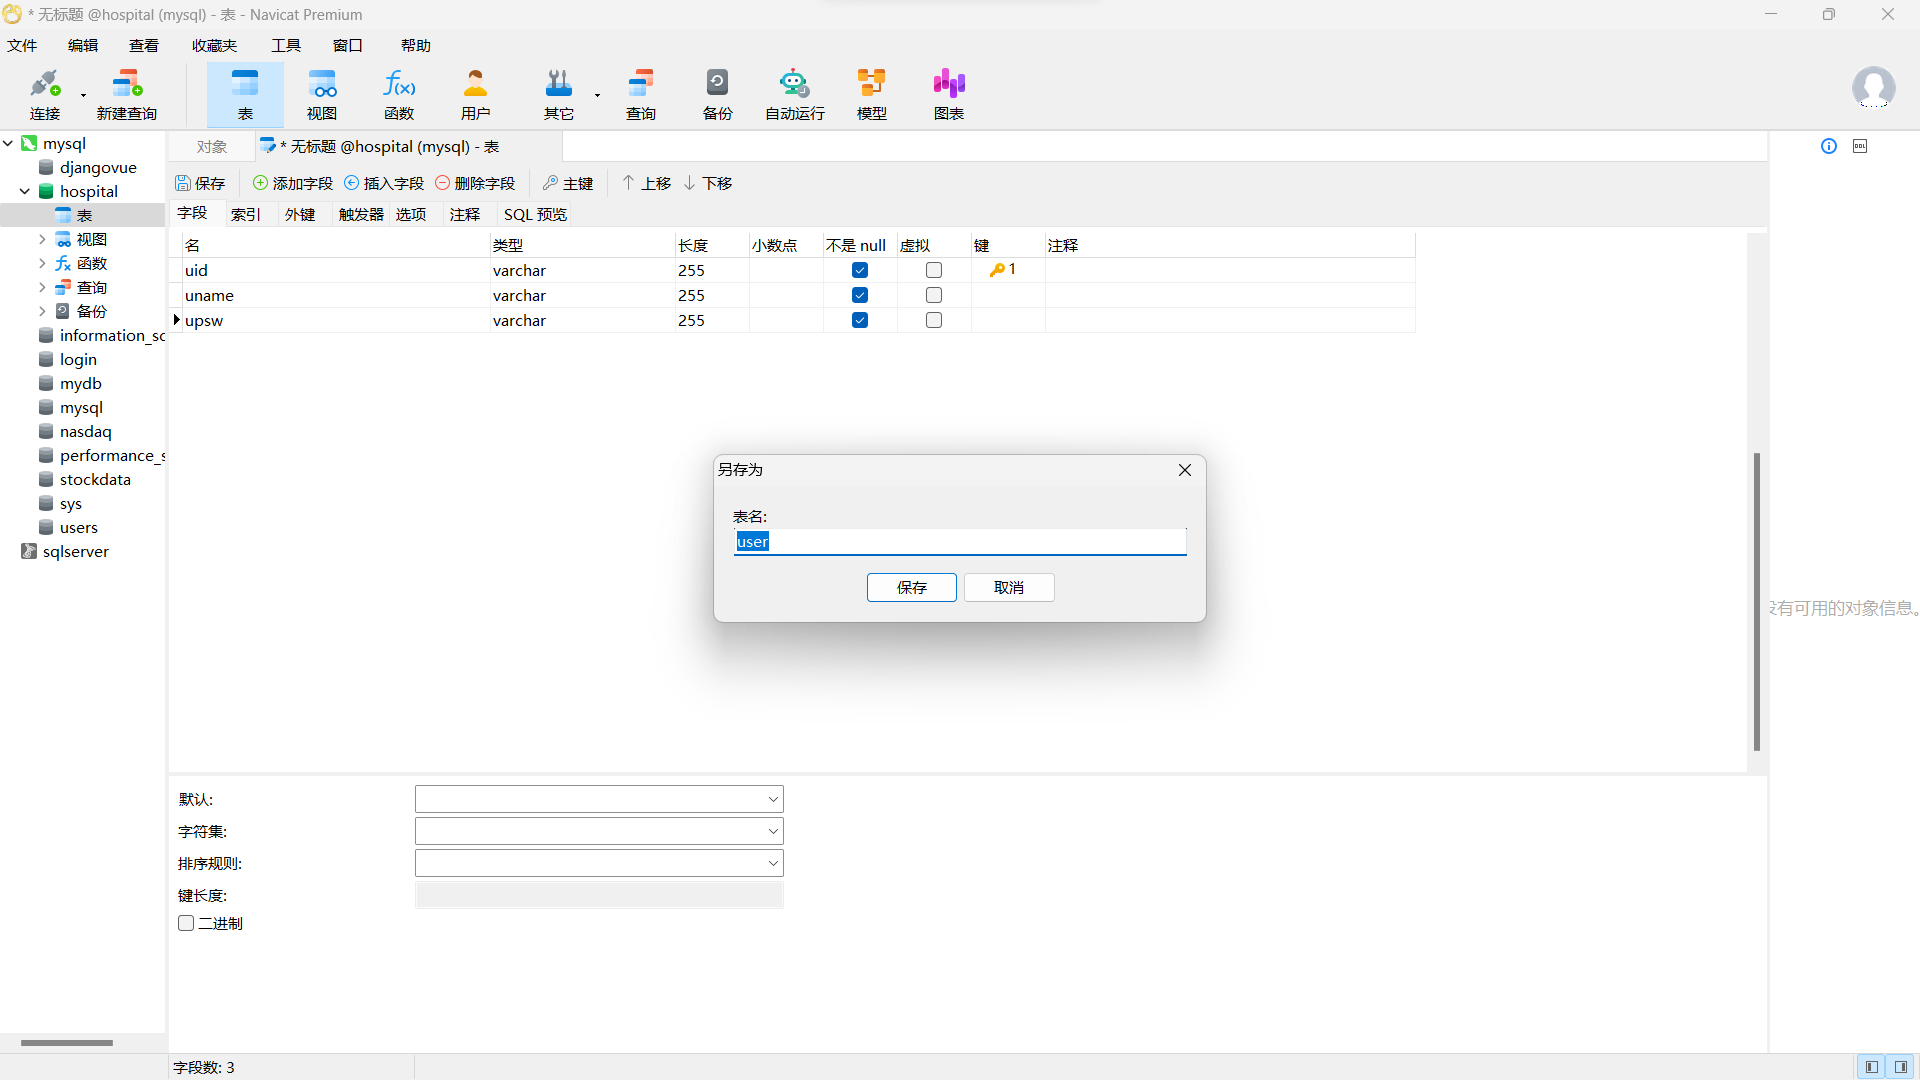
\includegraphics[width=1.0\textwidth]{imgs/5.png}
    \caption{user表}
\end{figure}

设计出的table结构如下

\begin{lstlisting}[frame=shadowbox]
+-------+--------------+------+-----+---------+-------+
| Field | Type         | Null | Key | Default | Extra |
+-------+--------------+------+-----+---------+-------+
| uid   | int(11)      | NO   | PRI | NULL    |       |
| uname | varchar(255) | NO   |     | NULL    |       |
| upsw  | varchar(255) | NO   |     | NULL    |       |
+-------+--------------+------+-----+---------+-------+
\end{lstlisting}

\newpage

\subsubsection{doctor表}

doctor表的主要字段有did,dname,dlevel,dinfo,departid,sex,ddetail分别代表医生id,医生姓名,医生职级,医生简介,医生所属科室id,医生性别,医生详细信息

\begin{figure}[htbp]
    \centering
    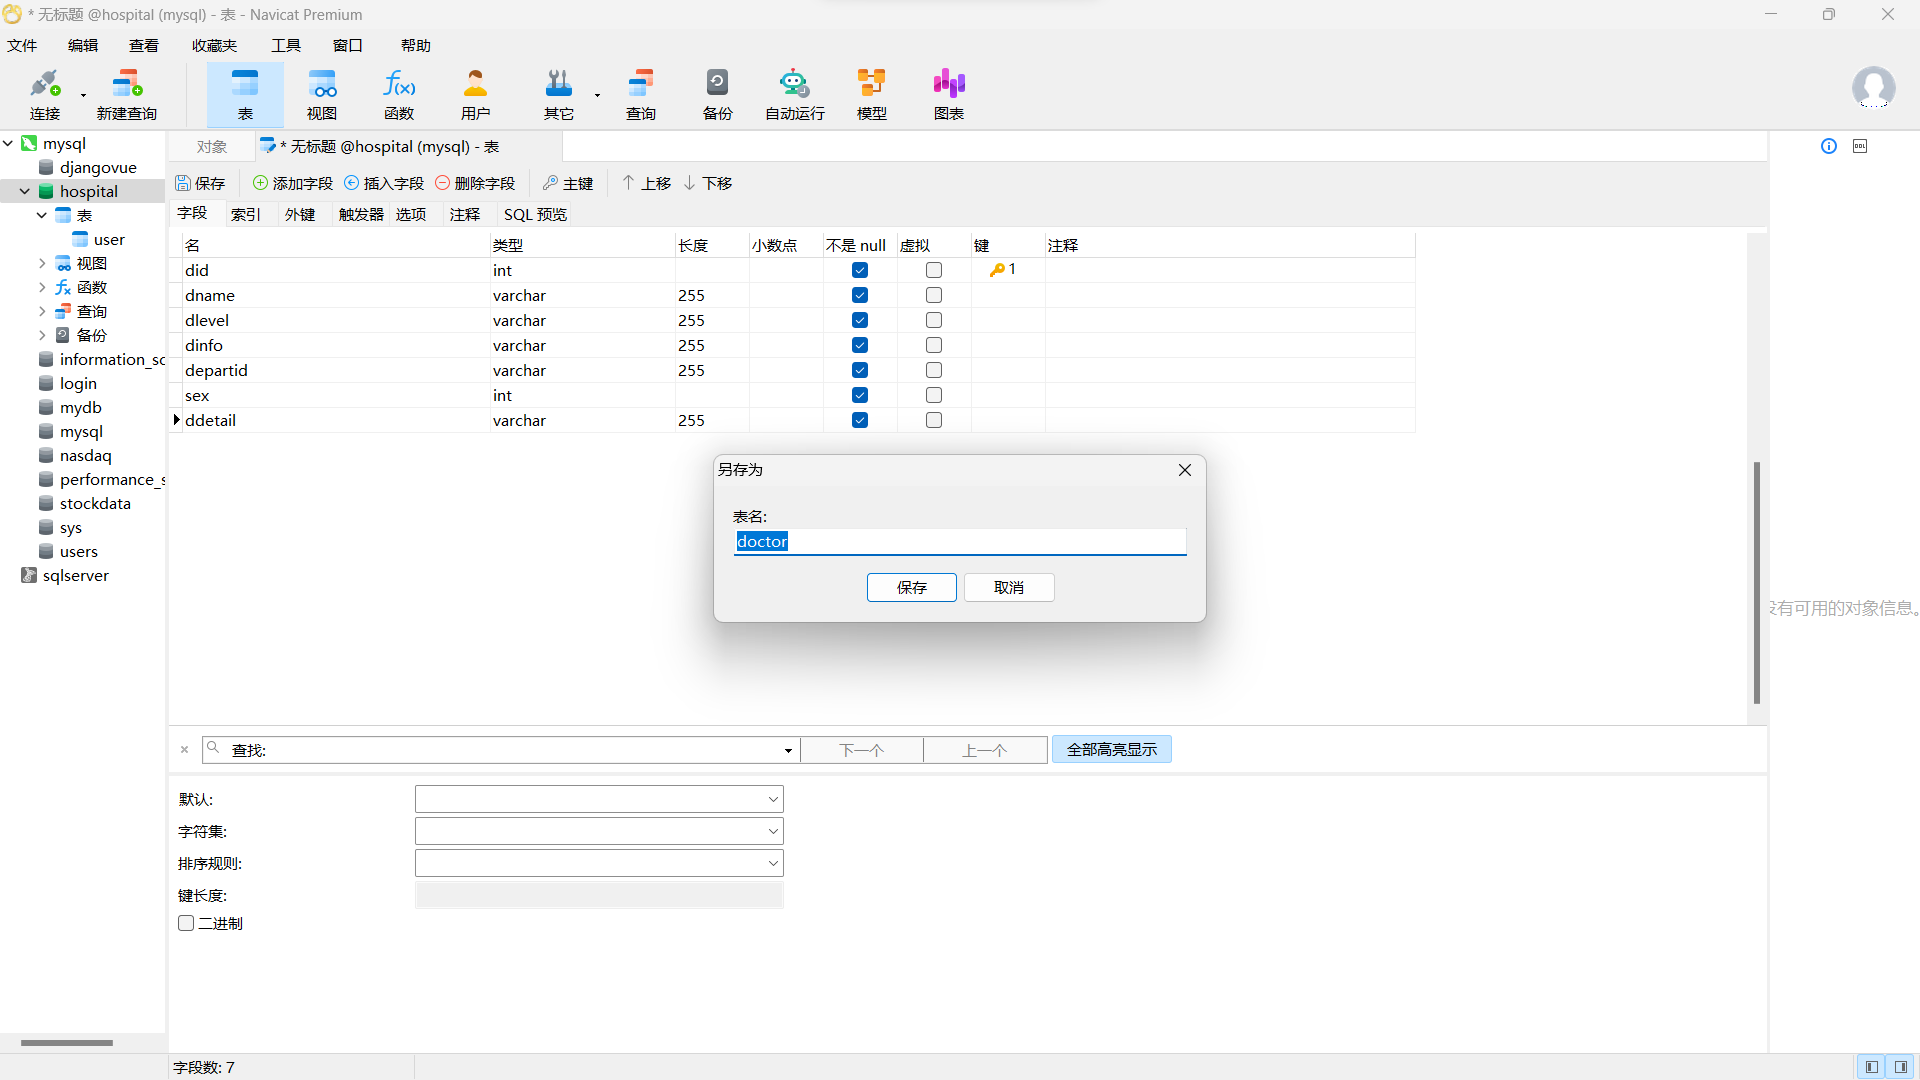
\includegraphics[width=1.0\textwidth]{imgs/6.png}
    \caption{doctor表}
\end{figure}

设计出的table结构如下

\begin{lstlisting}[frame=shadowbox]
+----------+--------------+------+-----+---------+-------+
| Field    | Type         | Null | Key | Default | Extra |
+----------+--------------+------+-----+---------+-------+
| did      | int(11)      | NO   | PRI | NULL    |       |
| dname    | varchar(255) | NO   |     | NULL    |       |
| dlevel   | varchar(255) | NO   |     | NULL    |       |
| dinfo    | varchar(255) | NO   |     | NULL    |       |
| departid | varchar(255) | NO   |     | NULL    |       |
| sex      | int(11)      | NO   |     | NULL    |       |
| ddetail  | varchar(255) | NO   |     | NULL    |       |
+----------+--------------+------+-----+---------+-------+
\end{lstlisting}

\newpage

\subsubsection{depart表}

depart表的主要字段有departid,departname,分别代表科室id,科室名称

\begin{figure}[htbp]
    \centering
    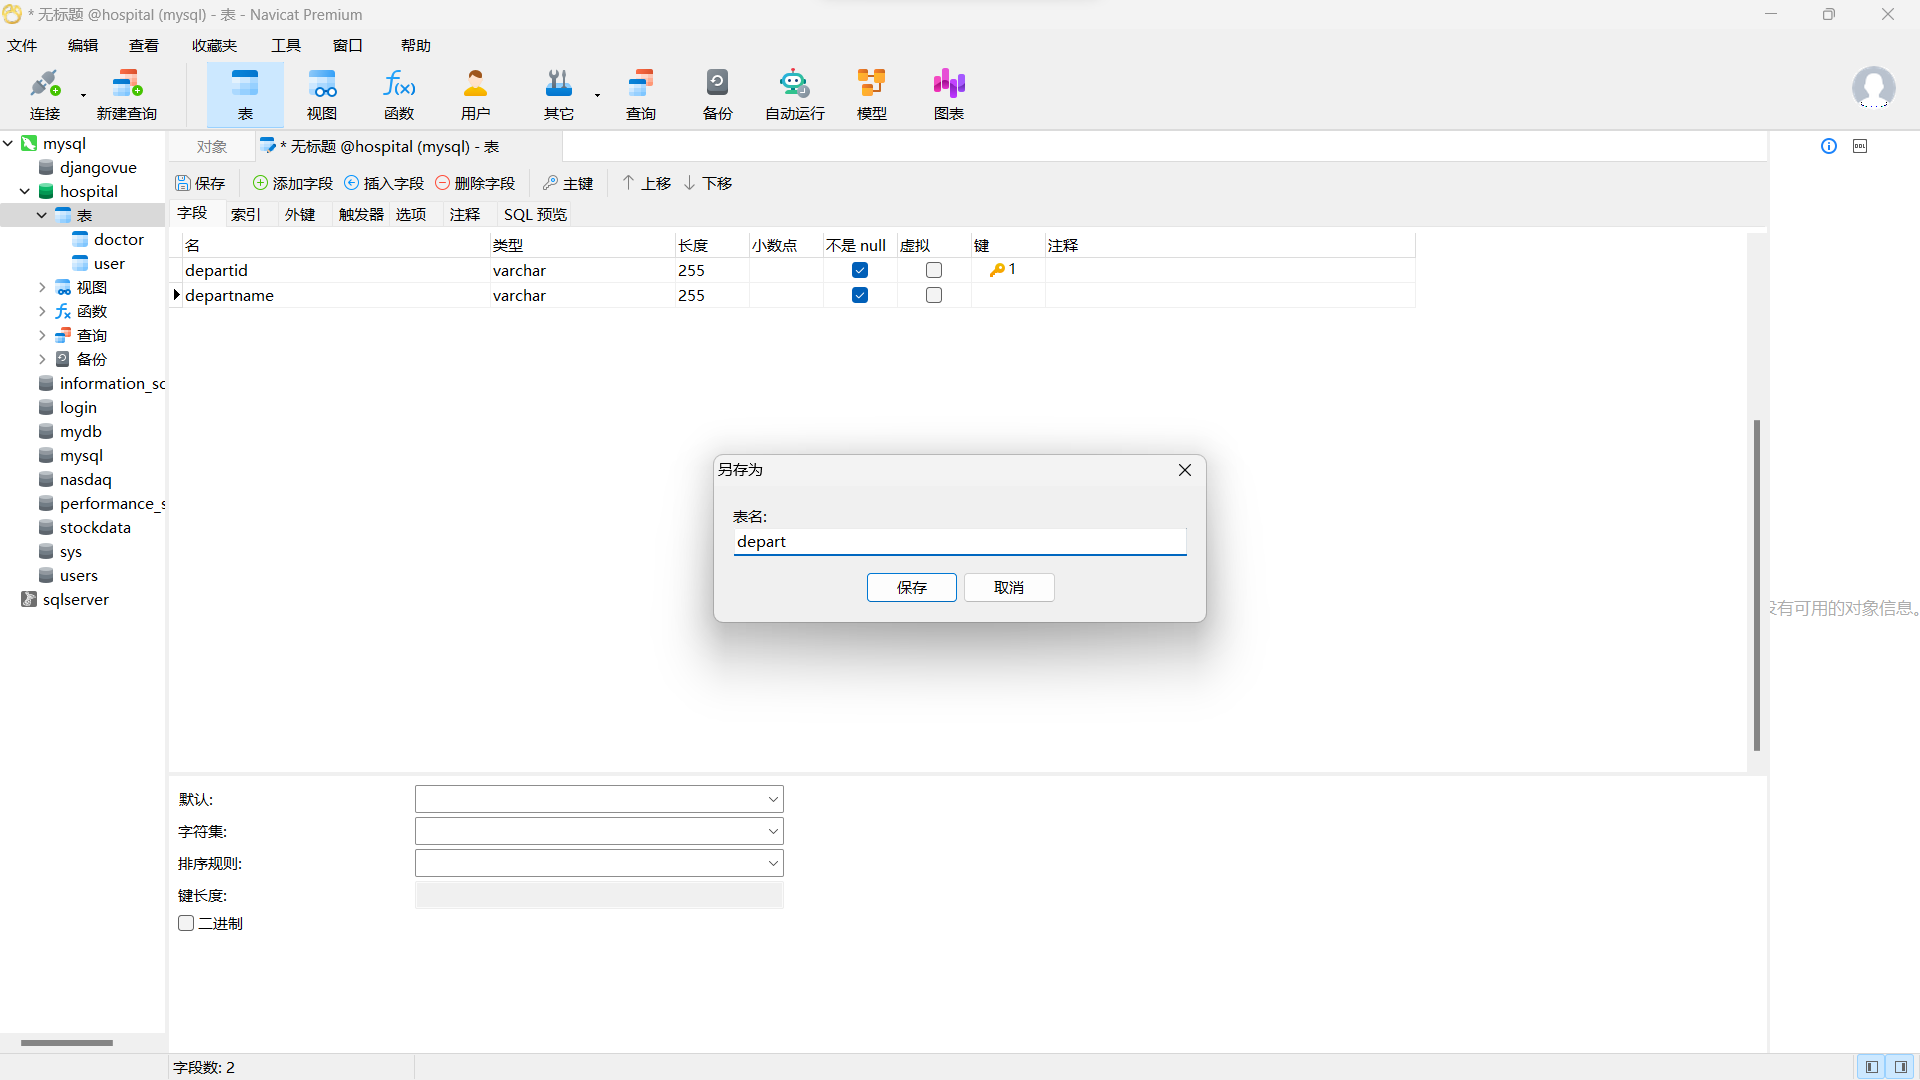
\includegraphics[width=1.0\textwidth]{imgs/7.png}
    \caption{depart表}
\end{figure}

设计出的table结构如下

\begin{lstlisting}[frame=shadowbox]
+------------+--------------+------+-----+---------+-------+
| Field      | Type         | Null | Key | Default | Extra |
+------------+--------------+------+-----+---------+-------+
| departid   | varchar(255) | NO   | PRI | NULL    |       |
| departname | varchar(255) | NO   |     | NULL    |       |
+------------+--------------+------+-----+---------+-------+
\end{lstlisting}

\newpage

\subsubsection{schedule表}

schedule表的主要字段有sid,did,time,price分别代表排班id,医生id,排班时间,挂号费

\begin{figure}[htbp]
    \centering
    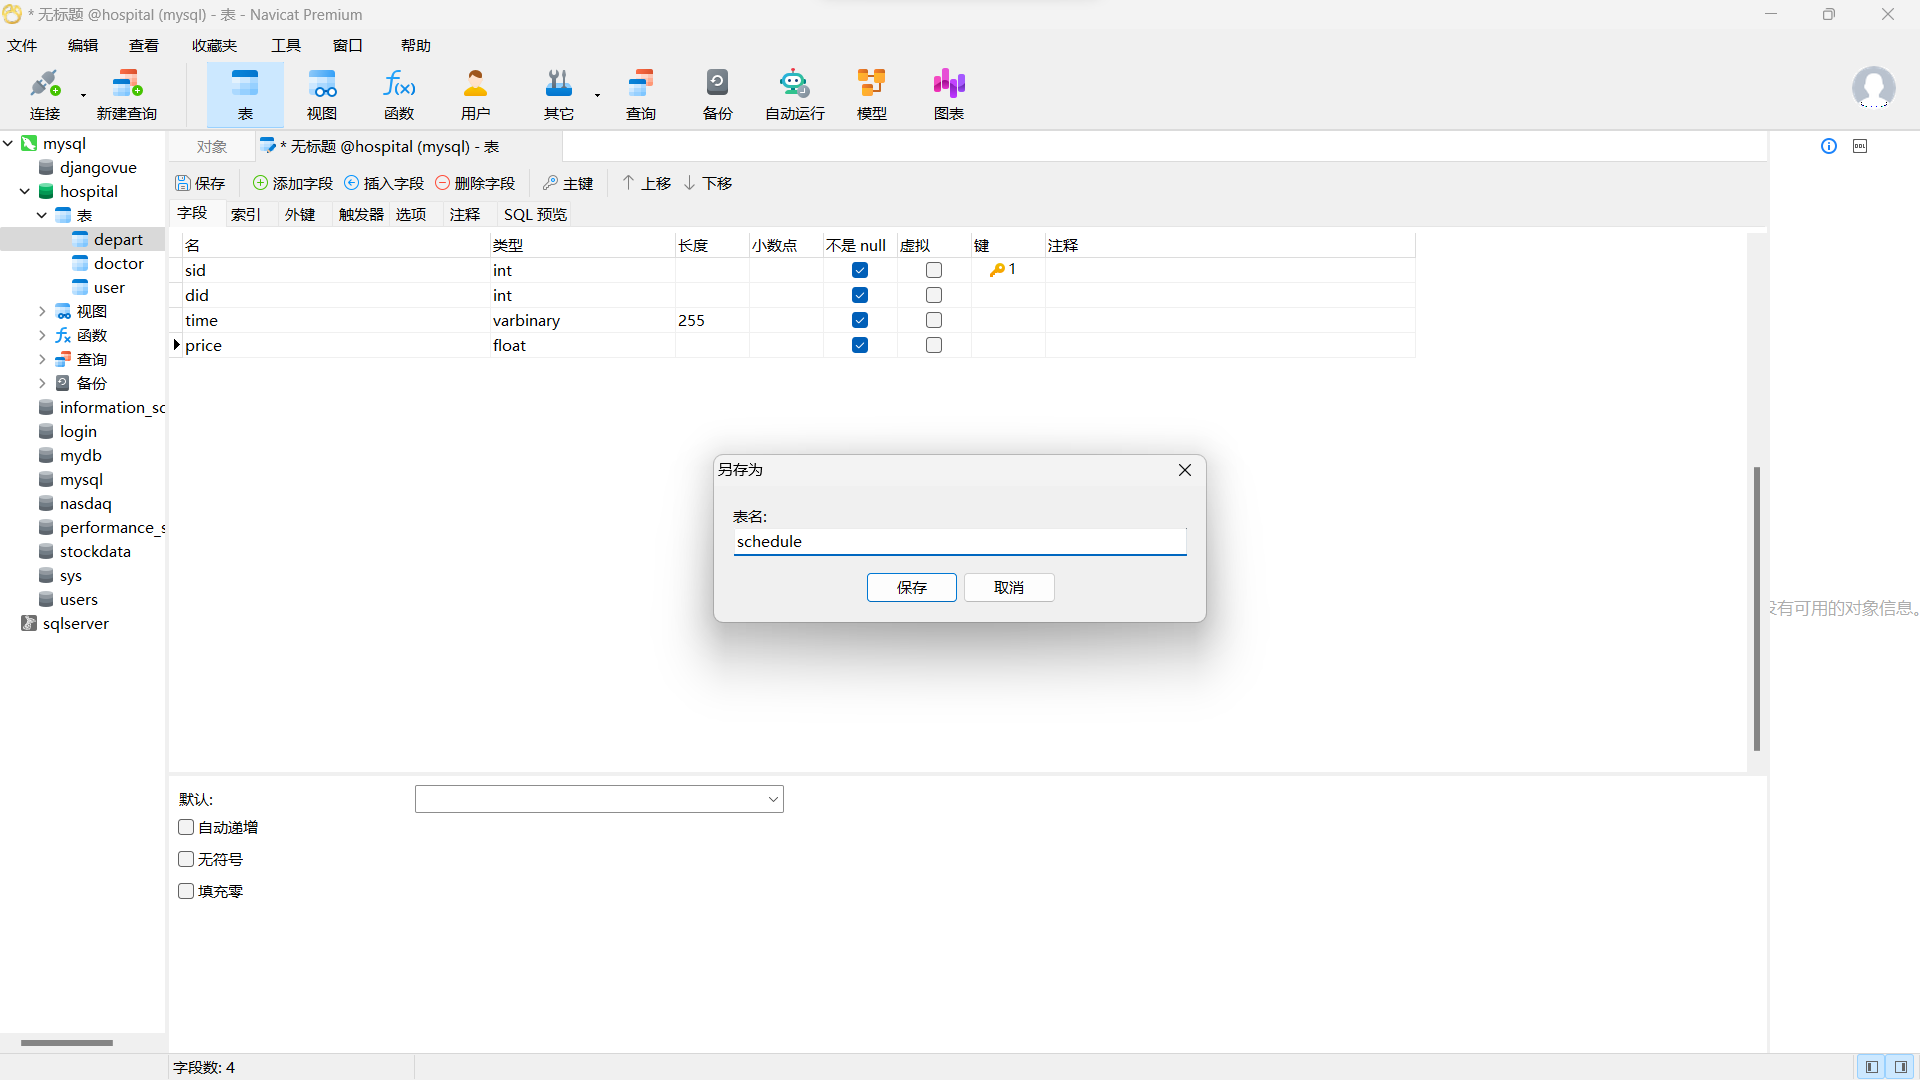
\includegraphics[width=1.0\textwidth]{imgs/8.png}
    \caption{schedule表}
\end{figure}

设计出的table结构如下

\begin{lstlisting}[frame=shadowbox]
+-------+----------------+------+-----+---------+-------+
| Field | Type           | Null | Key | Default | Extra |
+-------+----------------+------+-----+---------+-------+
| sid   | int(11)        | NO   | PRI | NULL    |       |
| did   | int(11)        | NO   |     | NULL    |       |
| time  | varbinary(255) | NO   |     | NULL    |       |
| price | float          | NO   |     | NULL    |       |
+-------+----------------+------+-----+---------+-------+
\end{lstlisting}

\newpage

\subsubsection{myorder表}

myorder表的主要字段有oid,sid,did,分别代表订单id,排班id,医生id

\begin{figure}[htbp]
    \centering
    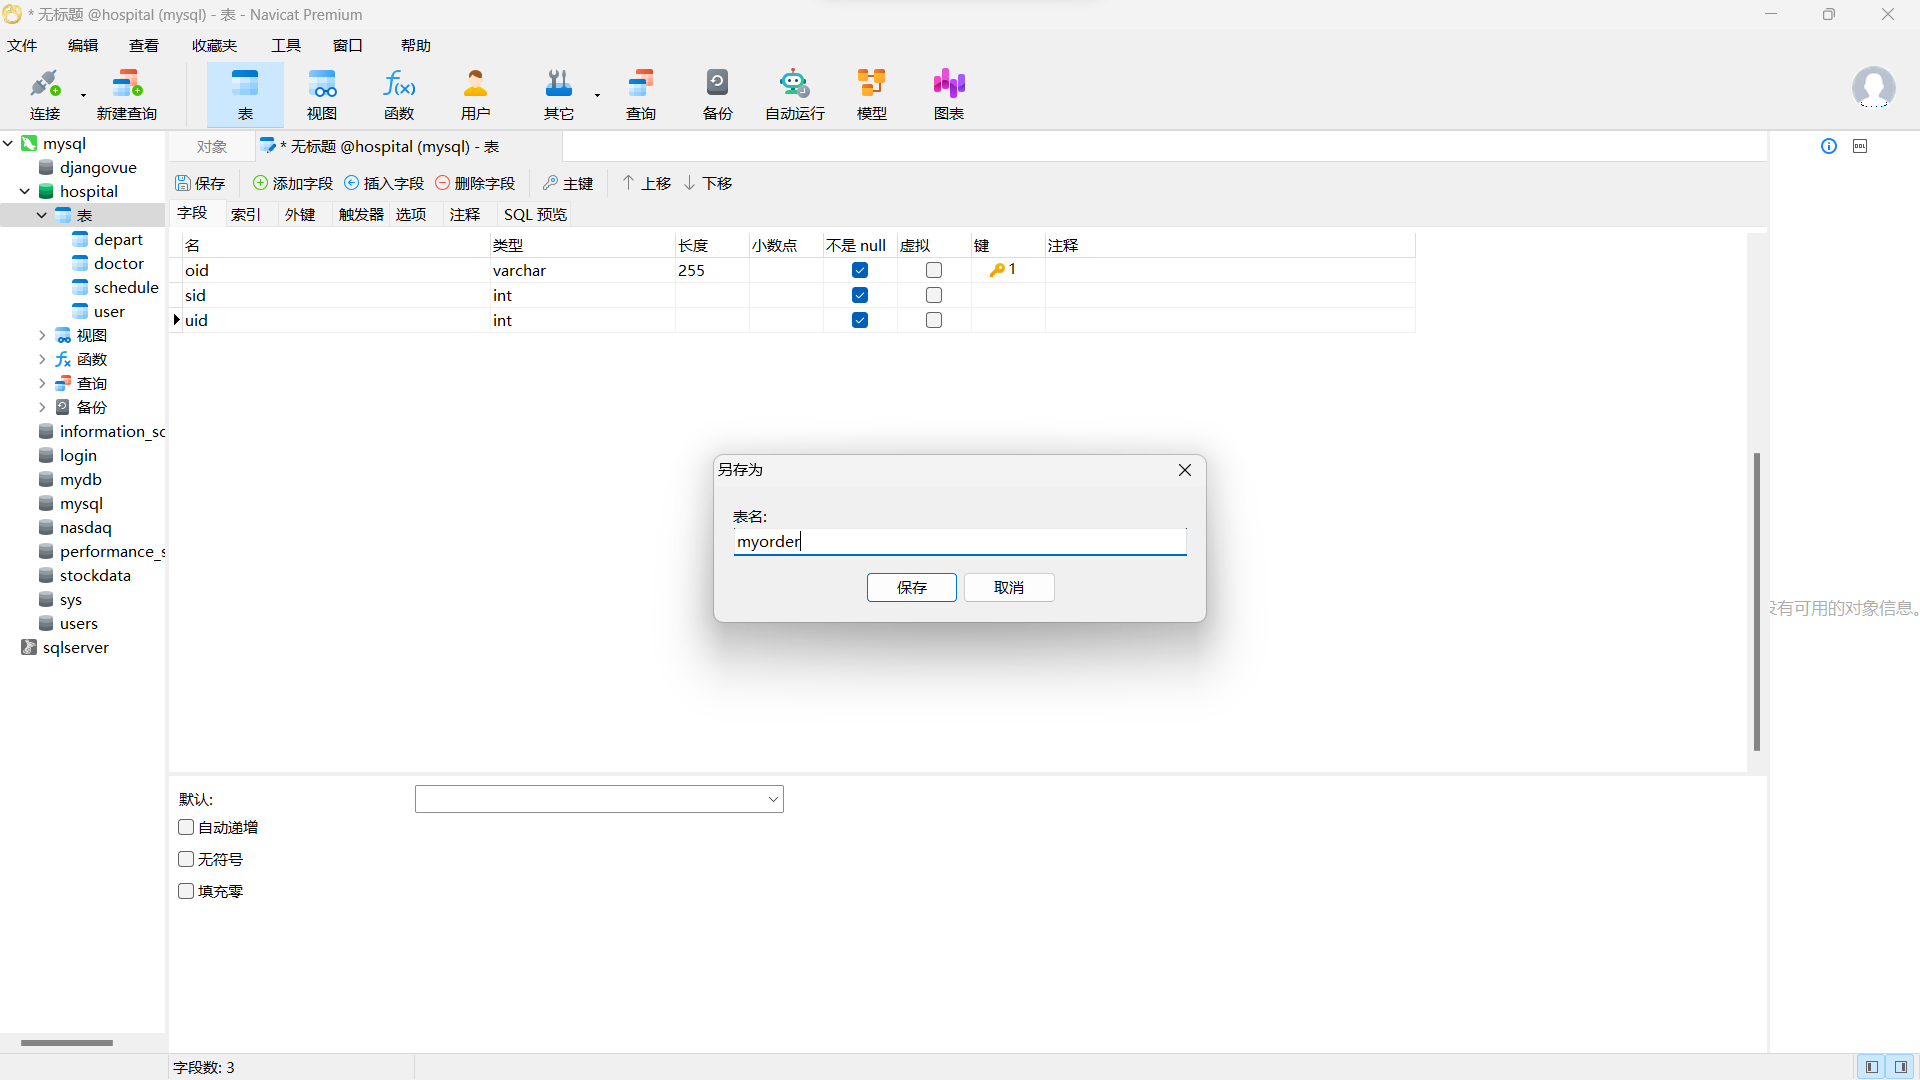
\includegraphics[width=1.0\textwidth]{imgs/9.png}
    \caption{myorder表}
\end{figure}

\begin{lstlisting}[frame=shadowbox]
+-------+--------------+------+-----+---------+-------+
| Field | Type         | Null | Key | Default | Extra |
+-------+--------------+------+-----+---------+-------+
| oid   | varchar(255) | NO   | PRI | NULL    |       |
| sid   | int(11)      | NO   |     | NULL    |       |
| uid   | int(11)      | NO   |     | NULL    |       |
+-------+--------------+------+-----+---------+-------+
\end{lstlisting}

\subsubsection{administrator表}
\begin{lstlisting}[frame=shadowbox]
+----------+--------------+------+-----+---------+-------+
| Field    | Type         | Null | Key | Default | Extra |
+----------+--------------+------+-----+---------+-------+
| user     | varchar(255) | NO   |     | NULL    |       |
| password | varchar(255) | NO   |     | NULL    |       |
+----------+--------------+------+-----+---------+-------+
\end{lstlisting}

\newpage

\subsection{Android看病预约客户端界面设计}
\subsubsection{界面设计流程图}
\begin{figure}[htbp]
    \centering
    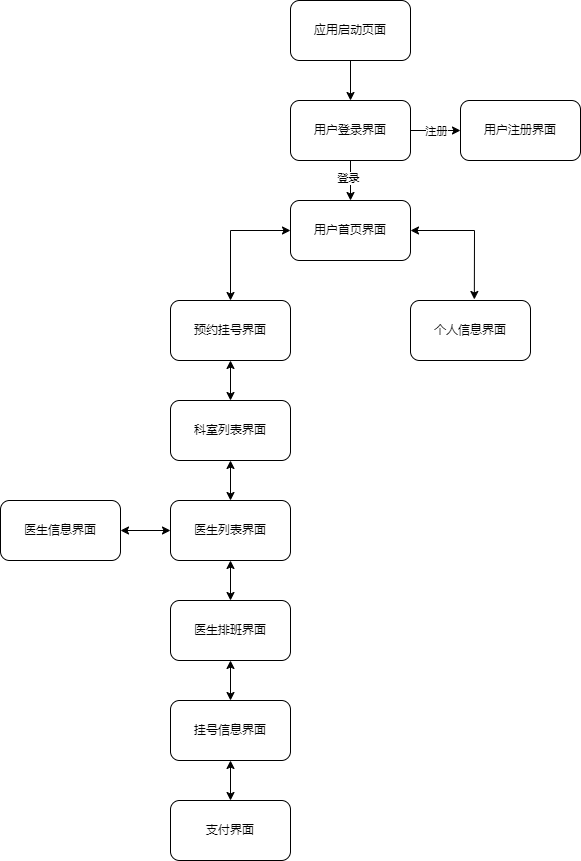
\includegraphics[width=0.7\textwidth]{imgs/3.png}
    \caption{Android看病预约客户端界面设计流程图}
\end{figure}

\newpage

\subsubsection{启动界面}
在程序启动的时候,需要一个启动界面,用于展示程序的logo,同时在启动界面中进行一些初始化操作,设置3s自动关闭启动界面。启动界面并不需要做的很复杂,只需要设计一个背景,然后添加一个按钮用于跳过启动界面即可。

设计的XML代码如下:

\begin{lstlisting}
<?xml version="1.0" encoding="utf-8"?>
<RelativeLayout xmlns:android="http://schemas.android.com/apk/res/android"
    xmlns:app="http://schemas.android.com/apk/res-auto"
    xmlns:tools="http://schemas.android.com/tools"
    android:layout_width="match_parent"
    android:layout_height="match_parent"
    tools:context=".ui.activity.SplashActivity"
    android:background="@mipmap/splashbg">
    <Button
        android:id="@+id/id_btn_skip"
        android:layout_alignParentRight="true"
        android:layout_alignParentTop="true"
        android:layout_width="wrap_content"
        android:layout_height="wrap_content"
        android:layout_gravity="right"
        android:layout_marginRight="32dp"
        android:layout_marginTop="32dp"
        android:background="@drawable/btn_bg_skip"
        android:paddingBottom="4dp"
        android:paddingLeft="12dp"
        android:paddingRight="12dp"
        android:paddingTop="4dp"
        android:text="跳过"
        android:minWidth="0dp"
        android:minHeight="0dp"
        android:textColor="#ffffff"
        android:textSize="14sp" />
</RelativeLayout>
\end{lstlisting}

\newpage

界面效果如下:

\begin{figure}[htbp]
    \centering
    
\includegraphics[width=0.6\textwidth]{imgs/10.png}
    \caption{启动界面}
\end{figure}

\subsubsection{登录界面}
登录界面需要设计一个背景,然后添加一个logo,接着添加两个输入框,分别用于输入用户名和密码,最后添加一个登录按钮。需要注意的是,在登录界面需要额外设置一个按钮,用于跳转到注册界面。
\begin{lstlisting}
<?xml version="1.0" encoding="utf-8"?>
<RelativeLayout xmlns:android="http://schemas.android.com/apk/res/android"
    xmlns:app="http://schemas.android.com/apk/res-auto"
    xmlns:tools="http://schemas.android.com/tools"
    android:layout_width="match_parent"
    android:layout_height="match_parent"
    tools:context=".ui.activity.LoginActivity"
    android:background="@mipmap/login_bg">
    <TextView
        android:id="@+id/id_tv_title"
        android:layout_width="wrap_content"
        android:layout_height="wrap_content"
        android:layout_centerHorizontal="true"
        android:layout_marginTop="90dp"
        android:text="掌上医院"
        android:textSize="40sp"
        android:textStyle="bold"></TextView>
    <EditText
        android:paddingLeft="20dp"
        android:id="@+id/id_et_uid"
        android:layout_width="match_parent"
        android:layout_height="56dp"
        android:layout_below="@id/id_tv_title"
        android:layout_marginTop="40dp"
        android:background="#44ffffff"
        android:hint="请输入账号"
        android:inputType="text"
        android:textColorHint="#070707" />
    <EditText
        android:paddingLeft="20dp"
        android:id="@+id/id_et_upsw"
        android:layout_width="match_parent"
        android:layout_height="56dp"
        android:layout_below="@id/id_et_uid"
        android:layout_marginTop="4dp"
        android:background="#44ffffff"
        android:hint="请输入密码"
        android:inputType="textWebPassword"
        android:textColorHint="#070707" />
    <Button
        android:id="@+id/id_btn_login"
        android:layout_width="match_parent"
        android:layout_height="wrap_content"
        android:layout_below="@id/id_et_upsw"
        android:layout_marginLeft="60dp"
        android:layout_marginTop="50dp"
        android:layout_marginRight="60dp"
        android:background="#87CEFA"
        android:text="登录"
        android:textSize="26sp" />
    <TextView
        android:id="@+id/id_tv_register"
        android:layout_width="wrap_content"
        android:layout_height="wrap_content"
        android:layout_below="@id/id_btn_login"
        android:layout_centerHorizontal="true"
        android:layout_marginTop="30dp"
        android:text="注册账号"
        android:textSize="18sp"
        android:textColor="#000000" />
</RelativeLayout>
\end{lstlisting}

以上是登录界面的XML代码,界面效果如下:

\begin{figure}[htbp]
    \centering
    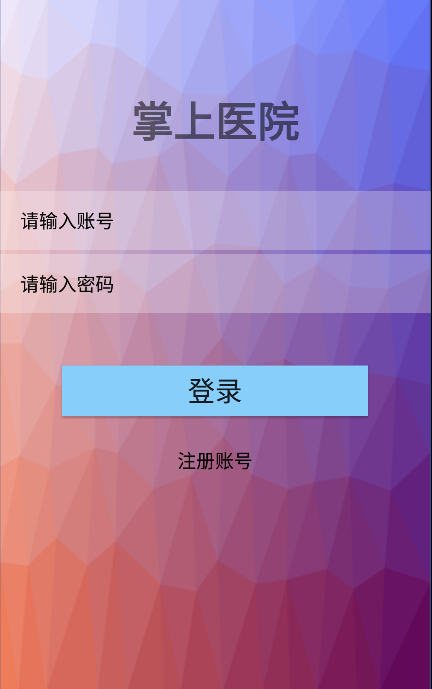
\includegraphics[width=0.4\textwidth]{imgs/11.png}
    \caption{登录界面}
\end{figure}

\subsubsection{注册界面}
注册界面需要设计一个背景,然后添加一个logo,接着添加四个输入框,分别用于输入用户姓名、用户名、密码、重复密码,最后添加一个注册按钮。需要注意的是,在注册界面需要额外设置一个按钮,用于跳转到登录界面。

这里的XML源码比较长,不进行展示,界面效果如下:

\begin{figure}[htbp]
    \centering
    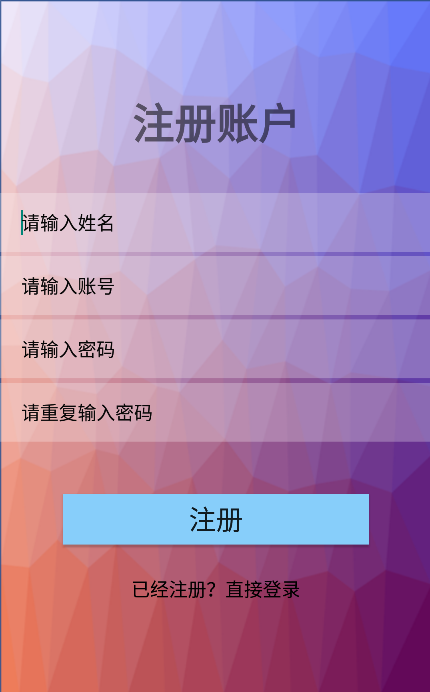
\includegraphics[width=0.4\textwidth]{imgs/12.png}
    \caption{注册界面}
\end{figure}

\subsubsection{用户首页}
用户首页设置一个背景,然后添加一个logo,接着添加三个按钮,分别用于跳转到预约挂号、我的信息、退出登录。目前只对用户首页进行了简单设计,并没有添加美化内容,只展示一个原型界面

实现的XML代码如下:

\begin{lstlisting}
    <?xml version="1.0" encoding="utf-8"?>
    <LinearLayout
        xmlns:android="http://schemas.android.com/apk/res/android"
        xmlns:app="http://schemas.android.com/apk/res-auto"
        xmlns:tools="http://schemas.android.com/tools"
        android:layout_width="match_parent"
        android:layout_height="match_parent"
        android:orientation="vertical"
        tools:context=".ui.activity.IndexActivity"
        android:background="@mipmap/login_bg"
        >
        <TextView
            android:id="@+id/welcome_uname"
            android:layout_marginTop="30dp"
            android:layout_width="match_parent"
            android:layout_height="50dp"
            android:text="李明,欢迎您!"
            android:gravity="center"
            android:textSize="26sp"
            android:textColor="@color/black"
            ></TextView>
        <Button
            android:id="@+id/btn1"
            android:layout_width="match_parent"
            android:layout_height="wrap_content"
            android:text="预约挂号"
            android:layout_marginTop="30dp"
            android:layout_marginLeft="20dp"
            android:layout_marginRight="20dp"
            android:textSize="26sp"
            android:background="#87CEFA"
            />
        <Button
            android:id="@+id/btn2"
            android:layout_width="match_parent"
            android:layout_height="wrap_content"
            android:text="我的信息"
            android:layout_marginTop="50dp"
            android:layout_marginLeft="20dp"
            android:layout_marginRight="20dp"
            android:textSize="26sp"
            android:background="#87CEFA"/>
        <Button
            android:id="@+id/btn3"
            android:layout_width="match_parent"
            android:layout_height="wrap_content"
            android:text="退出账号"
            android:layout_marginTop="50dp"
            android:layout_marginLeft="20dp"
            android:layout_marginRight="20dp"
            android:textSize="26sp"
            android:background="#87CEFA"/>
    </LinearLayout>
\end{lstlisting}

界面效果如下:

\begin{figure}[htbp]
    \centering
    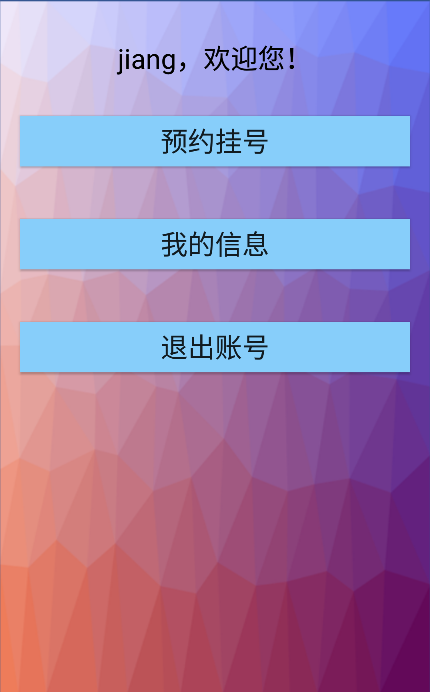
\includegraphics[width=0.4\textwidth]{imgs/13.png}
    \caption{用户首页}
\end{figure}

用户在预约挂号时,展现的科室列表、医生列表实际是一致的,在顶部标题处作区分,这里只展示科室列表设计。

\subsubsection{科室列表}
科室列表是一个列表,需要设计一个背景,然后添加一个logo,接着添加一个列表,用于展示科室列表

实现的XML代码如下:

\newpage

\begin{lstlisting}
<?xml version="1.0" encoding="utf-8"?>
<LinearLayout xmlns:android="http://schemas.android.com/apk/res/android"
    xmlns:app="http://schemas.android.com/apk/res-auto"
    xmlns:tools="http://schemas.android.com/tools"
    android:layout_width="match_parent"
    android:layout_height="match_parent"
    tools:context=".ui.activity.ChooseDepartActivity"
    android:orientation="vertical">
    <LinearLayout
        android:layout_width="wrap_content"
        android:layout_height="40dp">
        <ImageView
            android:id="@+id/btn_back"
            android:layout_width="40dp"
            android:layout_height="40dp"
            android:src="@mipmap/btn_back"></ImageView>
    </LinearLayout>
    <ListView
        android:id="@+id/depart_list_view"
        android:layout_width="match_parent"
        android:layout_height="match_parent"
        android:layout_marginLeft="20dp"
        android:layout_marginRight="20dp"></ListView>
</LinearLayout>
\end{lstlisting}

在列表的顶部作区分,部门、医生列表的顶部没有特殊设计,排班时间选择的时候,顶部打印了当前选择的医生信息。

\newpage

\subsection{Android看病预约客户端操作实现}
\subsubsection{启动界面}
用户点击软件图标之后,先进入启动页面,展示图标和软件名称,然后跳转到登录界面,右上角有一个跳过按钮,点击之后直接跳转到主界面。

实现activity为SplashActivity,点击“跳过”时,直接跳转到登录页面,具体如下:

\begin{lstlisting}[frame=shadowbox]
    public class SplashActivity extends AppCompatActivity {
    private Handler mHandler = new Handler();
    private Button mBtnSkip;
    private Runnable mRunnableToMain = new Runnable() {
        @Override
        public void run() {
            toLoginActivity();
        }
    };

    private void toLoginActivity() {
        Intent intent = new Intent(this, LoginActivity.class);
        startActivity(intent);
        finish();
    }

    @Override
    protected void onCreate(Bundle savedInstanceState) {
        super.onCreate(savedInstanceState);
        setContentView(R.layout.activity_splash);

        mBtnSkip = (Button) findViewById(R.id.id_btn_skip);
        mHandler.postDelayed(mRunnableToMain, 3000);

        mBtnSkip.setOnClickListener(new View.OnClickListener() {
            @Override
            public void onClick(View view) {
                mHandler.removeCallbacks(mRunnableToMain);
                toLoginActivity();
            }
        });

    }
}

\end{lstlisting}

\subsubsection{登录/注册界面}
用户经过启动页面之后,进入登录页面,用户根据自身需求选择:跳转到注册界面,或直接输入账号密码进行登录。

若跳转到注册界面,用户输入账号密码,点击注册按钮,将账号密码发送到服务器,服务器返回注册成功或失败的信息,若成功,则跳转到登录界面,若失败,则提示用户注册失败。

若直接登录,则用户输入账号密码,点击登录按钮,将账号密码发送到服务器,服务器返回登录成功或失败的信息,若成功,则跳转到主界面,若失败,则提示用户登录失败。

具体的流程图如下:

\begin{figure}[htbp]
    \centering
    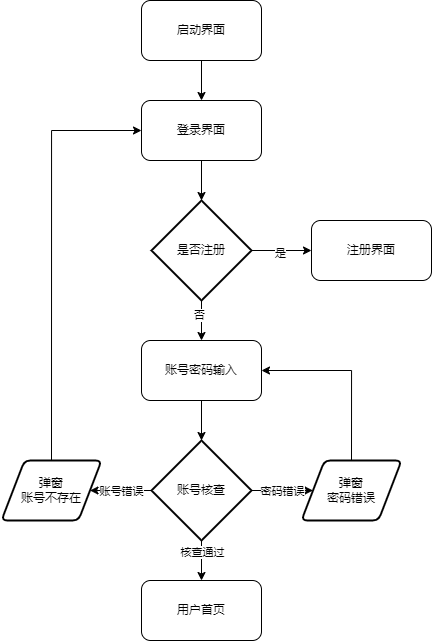
\includegraphics[width=0.6\textwidth]{imgs/14.png}
    \caption{登录/注册流程图}
\end{figure}

\newpage

在应用端只负责提交数据,不负责验证数据,验证数据的工作交给服务器端,也就是说应用端只需要提取输入框的输入即可,返回的提示用toast实现,具体代码如下:

\begin{lstlisting}[frame=shadowbox]
    public String requestDataByPost(String urlString) {
        String result = null;
        try {
            URL url = new URL(urlString);
            HttpURLConnection connection = (HttpURLConnection) url.openConnection();
            connection.setConnectTimeout(30000);
            connection.setRequestMethod("POST");

            // 设置运行输入,输出:
            connection.setDoOutput(true);
            connection.setDoInput(true);
            // Post方式不能缓存,需手动设置为false
            connection.setUseCaches(false);
            connection.connect();

            // 我们请求的数据:
            String data = "uid=" + URLEncoder.encode(uid, "UTF-8")
                    + "&upsw=" + URLEncoder.encode(upsw, "UTF-8");
            // 获取输出流
            OutputStream out = connection.getOutputStream();
            out.write(data.getBytes());
            out.flush();
            out.close();

            int responseCode = connection.getResponseCode();
            if (responseCode == HttpURLConnection.HTTP_OK) {
                InputStream inputStream = connection.getInputStream();
                result = NetUtil.streamToString(inputStream);

                user = new Gson().fromJson(result,User.class);


            } else {
                String responseMessage = connection.getResponseMessage();

            }


            connection.disconnect();
            return result;
        } catch (MalformedURLException e) {
            e.printStackTrace();
        } catch (IOException e) {
            e.printStackTrace();
        }
        return null;
    }
\end{lstlisting}

注册与登录类似,唯一不同的是请求的数据不同,注册需要提交的数据有uid,upsw,uname,而登录只需要提交uid,upsw即可。

\begin{lstlisting}[frame=shadowbox]
    String data ="uname=" + URLEncoder.encode(uname, "UTF-8") +  "&uid=" + URLEncoder.encode(uid, "UTF-8")
    + "&upsw=" + URLEncoder.encode(upsw, "UTF-8");
\end{lstlisting}

\subsubsection{预约界面}
预约分为三步
\begin{enumerate}
    \item 选择科室
    \item 选择医生
    \begin{itemize}
        \item 查看医生详细介绍
    \end{itemize}
    \item 选择时间
\end{enumerate}

\textbf{选择科室}

向后端请求科室数据,获取科室List,然后将科室List展示在列表中,用户点击列表中的某一项,跳转到医生列表界面,同时将用户选择的科室信息传递到医生列表界面,用于向后端请求医生列表数据。

涉及到的数据流:数据库->服务器->客户端。由于网络操作速度慢,需要将网络请求操作写在另外的线程中,得到数据之后,显示在客户端界面上。

\begin{enumerate}
    \item 向服务器请求科室数据
    \\编写一个类,继承自AsyncTask,完成异步任务
    \begin{lstlisting}[frame=shadowbox]
    public class DepartAsyncTask extends AsyncTask<Void,Void, String> {

        @Override
        protected String doInBackground(Void... params) {
            result = NetUtil.requestDataByGet(baseurl);
            return result;
        }

        @Override
        protected void onPostExecute(String result) {
            super.onPostExecute(result);
            Gson gson = new Gson();
            departs = gson.fromJson(result, new TypeToken<List<Depart>>() {}.getType());
            departListView.setAdapter(new DepartListAdapter( departs));
        }
    }
    \end{lstlisting}

    \begin{itemize}
        \item 重写doInBackground方法,该方法在另外的线程中执行,用于向服务器请求数据,然后返回数据
        \item 重写onPostExecute方法,该方法在主线程中执行,将数据从json格式转换成Gson格式,然后使用适配器将数据展示在列表中
    \end{itemize}

    \item 将数据展示在列表中
    \\采用ListView控件,需要编写一个适配器。将数据展示在列表中,在layout文件夹中新建一个item\_depart\_list\_view.xml文件,用于展示列表中的每一项,然后编写一个适配器,将数据展示在列表中,同时为每一项添加点击事件,点击之后跳转到医生列表界面,同时将用户选择的科室信息传递到医生列表界面,用于向后端请求医生列表数据。

    实现步骤如下:

    \begin{enumerate}
        \item 在layout中创建ListView
        \item 创建每一行layout
        \item 创建每一行数据
        \item 用适配器将数据展示在ListView中
    \end{enumerate}

    编写一个类继承BaseAdapter,实现适配器的功能,为每个item添加点击监听时间,并将被点击的科室depart数据用intent传递给下一个activity。

    \begin{lstlisting}[frame=shadowbox]
        public class DepartListAdapter extends BaseAdapter{
            private List<Depart> mdeparts;
            DepartListAdapter(List<Depart> departs){
                mdeparts = departs;
            }
            @Override
            public int getCount() {
                return mdeparts.size();
            }
    
            @Override
            public Object getItem(int i) {
                return mdeparts.get(i);
            }
    
            @Override
            public long getItemId(int i) {
                return mdeparts.get(i).getDepartid();
            }
    
            @Override
            public View getView(int i, View view, ViewGroup viewGroup) {
    
                if(view == null){
                    LayoutInflater layoutInflater = (LayoutInflater)getSystemService(Context.LAYOUT_INFLATER_SERVICE);
                    view = layoutInflater.inflate(R.layout.item_depart_list_view,null);
                }
                TextView departName = view.findViewById(R.id.depart_name_tv);
                departName.setText(mdeparts.get(i).getDepartname());
    
                departName.setOnClickListener(new View.OnClickListener() {
                    @Override
                    public void onClick(View view) {
                        Intent intent = new Intent(ChooseDepartActivity.this,ChooseDoctorActivity.class);
                        intent.putExtra("depart",new Gson().toJson(mdeparts.get(i)));
                        startActivity(intent);
    
    
                    }
                });
    
                return view;
            }
        }
    \end{lstlisting}

\end{enumerate}

\begin{figure}[htbp]
    \centering
    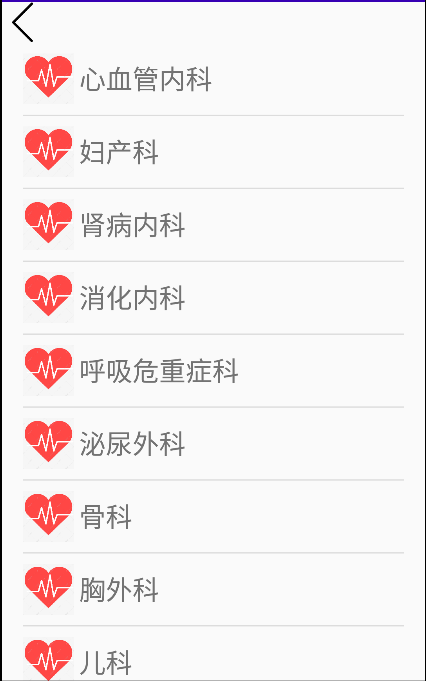
\includegraphics[width=0.6\textwidth]{imgs/21.png}
    \caption{选择科室界面}
\end{figure}

\newpage

\textbf{选择医生}

医生列表界面接收科室列表界面通过intent传递过来的科室信息,然后向后端请求医生数据,获取医生List,然后将医生List展示在列表中,列表实现的功能有

\begin{enumerate}
    \item 用户点击列表中的某一项,跳转到医生详细信息界面
    \item 用户点击预约按钮,跳转到选择时间界面
\end{enumerate}

因此需要对两个事件进行监听

\begin{lstlisting}[frame=shadowbox]
    public class DoctorListAdapter extends BaseAdapter {
        private List<Doctor> mdoctors;
        ...
        @Override
        public View getView(int i, View view, ViewGroup viewGroup) {

            ...

            if(mdoctors.get(i).getSex()==1){
                dimg.setImageResource(R.mipmap.doctor_male);
            }
            else{
                dimg.setImageResource(R.mipmap.doctor_female);
            }
            dname.setText(mdoctors.get(i).getDname());
            dlevel.setText(mdoctors.get(i).getDlevel());
            dinfo.setText(mdoctors.get(i).getDinfo());


            btn_ddetail.setOnClickListener(new View.OnClickListener(){
                @Override
                public void onClick(View view) {
                    Intent intent = new Intent(ChooseDoctorActivity.this,DoctorDetailActivity.class);
                    intent.putExtra("doctor",new Gson().toJson(mdoctors.get(i)));
                    startActivity(intent);
                }
            });

            btn_reverse.setOnClickListener(new View.OnClickListener() {
                @Override
                public void onClick(View view) {
                    Intent intent = new Intent(ChooseDoctorActivity.this,ChooseTimeActivity.class);
                    intent.putExtra("doctor",new Gson().toJson(mdoctors.get(i)));
                    startActivity(intent);
                }
            });

            return view;
        }
    }
\end{lstlisting}

\begin{figure}[htbp]
    \begin{minipage}[t]{0.45\textwidth}
        \centering
        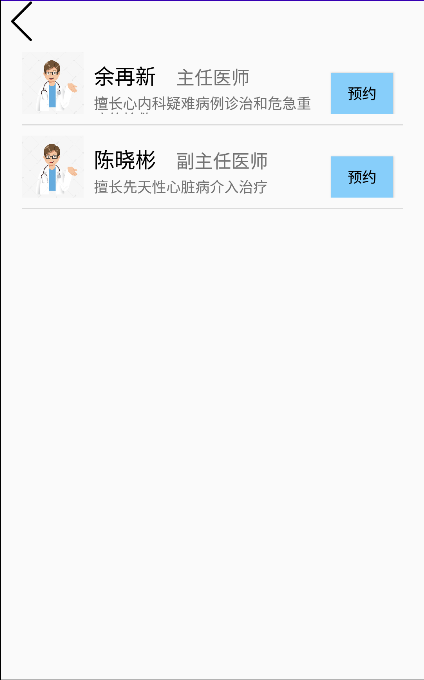
\includegraphics[width=0.9\textwidth]{imgs/22.png}
        \caption{选择医生界面}
    \end{minipage}%
    \begin{minipage}[t]{0.45\textwidth}
        \centering
        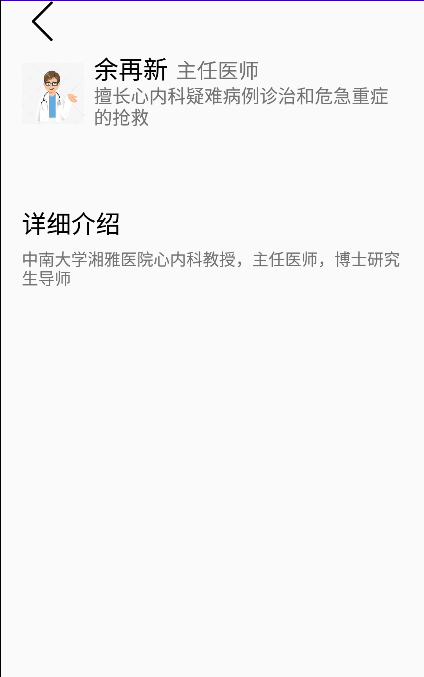
\includegraphics[width=0.9\textwidth]{imgs/23.png}
        \caption{医生详细信息界面}
    \end{minipage}
\end{figure}

\newpage

\textbf{医生详细介绍}

医生详细介绍界面只是简单的展示医生的详细介绍,没有其他操作,只需要获取医生的数据,然后展示即可。

\begin{lstlisting}[frame=shadowbox]
    protected void onCreate(Bundle savedInstanceState) {
        super.onCreate(savedInstanceState);
        setContentView(R.layout.activity_doctor_detail);
        String doctorJson = getIntent().getStringExtra("doctor");
        doctor =  new Gson().fromJson(doctorJson, Doctor.class);
        Log.e("DoctorDetailActivity","传来的数据:"+ doctor);
        ImageView dimg = findViewById(R.id.dimg);
        TextView dname = findViewById(R.id.dname);
        TextView dlevel = findViewById(R.id.dlevel);
        TextView dinfo = findViewById(R.id.dinfo);
        TextView ddetail = findViewById(R.id.ddetail);
        if(doctor.getSex()==1){
            dimg.setImageResource(R.mipmap.doctor_male);
        }
        else{
            dimg.setImageResource(R.mipmap.doctor_female);
        }
        dname.setText(doctor.getDname());
        dlevel.setText(doctor.getDlevel());
        dinfo.setText(doctor.getDinfo());
        ddetail.setText(doctor.getDdetail());
        ImageView btn_back = findViewById(R.id.btn_back);
        btn_back.setOnClickListener(new View.OnClickListener() {
            @Override
            public void onClick(View view) {
                Intent intent = new Intent(DoctorDetailActivity.this,ChooseDoctorActivity.class);
                intent.putExtra("departid",doctor.getDdepartid());
                startActivity(intent);
            }
        });
    }
\end{lstlisting}

\newpage

\textbf{选择时间}

根据选择的医生,向后端请求排班时间数据,获取排班时间List,然后将排班时间List展示在列表中,用户点击列表中的某一项,跳转到支付界面,同时将用户选择的排班时间信息传递到支付界面,用于向后端请求支付数据。实际的获取列表方式和前面一致,修改传入参数就可以了。

\begin{figure}[htbp]
    \centering
    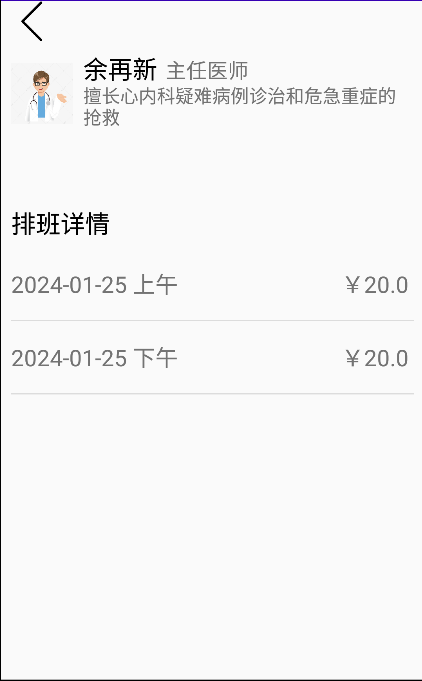
\includegraphics[width=0.6\textwidth]{imgs/24.png}
    \caption{选择时间界面}
\end{figure}

\newpage

\subsubsection{支付界面}
支付的实际功能需要调用支付系统的API,这一部分难以实现,故只做了一个简单的界面,用于展示用户选择的预约信息,用户点击支付按钮,提示用户支付成功,然后跳转到用户首页,对于支付操作进行了简单的模拟。

支付界面展示之前的选择结果,设置两个按钮监听器,一个用于支付,一个用于取消支付,点击支付按钮,向后端请求支付数据,获取支付数据,然后调用支付接口,调用成功则提示用户支付成功,调用失败则提示用户支付失败,点击取消支付按钮,直接跳转到用户首页。

\begin{figure}[htbp]
    \centering
    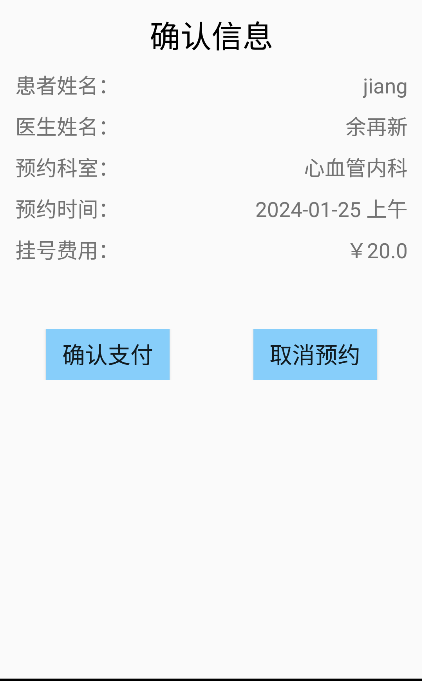
\includegraphics[width=0.6\textwidth]{imgs/25.png}
    \caption{支付界面}
\end{figure}

这里看一下两个按钮的监听器,支付按钮的监听器如下:

\begin{lstlisting}[frame=shadowbox]
    pay_yes.setOnClickListener(new View.OnClickListener() {
            @Override
            public void onClick(View view) {
                baseurl += "?sid="+schedule.getSid()+"&uid="+user.getUid();
                Toast.makeText(getBaseContext(),"预约挂号成功!",Toast.LENGTH_SHORT).show();
                new PayActivity.PayAsyncTask().execute();

            }
        });
\end{lstlisting}

取消支付按钮的监听器如下:

\begin{lstlisting}[frame=shadowbox]
    pay_no.setOnClickListener(new View.OnClickListener() {
        @Override
        public void onClick(View view) {
            Toast.makeText(getBaseContext(),"预约挂号取消成功!",Toast.LENGTH_SHORT).show();
            Intent intent = new Intent(PayActivity.this,ChooseTimeActivity.class);
            intent.putExtra("doctor",new Gson().toJson(doctor));
            startActivity(intent);
        }
    });
\end{lstlisting}

\subsubsection{我的信息界面}
主要用于显示已经预约的结果,向后端请求预约数据,获取预约数据,然后将预约数据展示在列表中,用户点击列表中的某一项,跳转到预约详情界面,同时将用户选择的预约信息传递到预约详情界面,用于展示预约详情。

\begin{lstlisting}[frame=shadowbox]
    protected void onCreate(Bundle savedInstanceState) {
        super.onCreate(savedInstanceState);
        setContentView(R.layout.activity_my_info);
        user =  new Gson().fromJson( getIntent().getStringExtra("user"), User.class);
        TextView uname = findViewById(R.id.welcome_uname);
        ImageView btn_back = findViewById(R.id.btn_back);
        myInfoListView = findViewById(R.id.myinfo_list_view);
        btn_back.setOnClickListener(new View.OnClickListener() {
            @Override
            public void onClick(View view) {
                Intent intent = new Intent(MyInfoActivity.this,IndexActivity.class);
                intent.putExtra("user",new Gson().toJson(user));
                startActivity(intent);
            }
        });
        if(user!=null){
            uname.setText(""  + user.getUname() + ",欢迎您!");
        }
        baseurl= baseurl + "?uid="+user.getUid();
        new MyInfoActivity.MyinfoAsyncTask().execute();
    }
\end{lstlisting}

\begin{figure}[htbp]
    \centering
    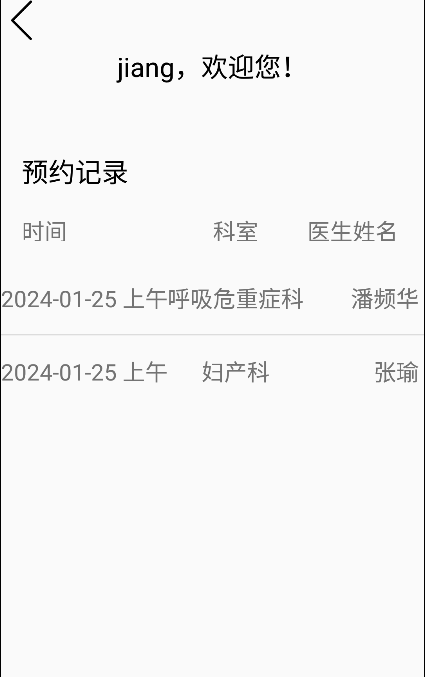
\includegraphics[width=0.4\textwidth]{imgs/26.png}
    \caption{我的信息界面}
\end{figure}

\newpage

\subsection{配置android网络}
android 和web 服务器的数据交互,涉及到android 的网络相关操作,可以选择使用第三方库或者自己编写简单的代码实现。我采用了自己编写代码,并抽取到工具类NetUtil中。

\subsubsection{配置baseurl}
首先配置类Config,里面存储了访问服务器用的url中基础的部分,本实践采用了主机作服务器,其中由于主机连接WLAN,而非有线的Ethernet,因此ip地址会变化;对于实际的工程来说,服务器的ip应当是固定的,不存在以上问题。

\begin{lstlisting}[frame=shadowbox]
    public class Config {
        public static String baseUrl ="http://100.67.123.30:8080/PalmHospitalService_war_exploded/";
    }
\end{lstlisting}

这样在其他类中,只需要将url加上这一部分,修改代码很方便。

\subsubsection{编写工具类NetUtil}
接着编写工具类NetUtil:由于数据量不大,我们都采用Get 的请求方式,将参数添加在url 末尾。编写函数requestDataByGet:参数url,进行HttpURLConnection 的相关设置,获取请求的返回码,判断是否成功等等

\begin{lstlisting}[frame=shadowbox]
    package com.example.palmhospital.utils;

    import android.util.Log;
    import java.io.ByteArrayOutputStream;
    import java.io.IOException;
    import java.io.InputStream;
    import java.net.HttpURLConnection;
    import java.net.MalformedURLException;
    import java.net.URL;
    public class NetUtil {
        public static String requestDataByGet(String urlString) {
            String result = null;
            try {
                URL url = new URL(urlString);
                HttpURLConnection connection = (HttpURLConnection) url.openConnection();
                connection.setConnectTimeout(30000);        // 设置超时时间
                connection.setRequestMethod("GET");  // 请求的方法类型:GET POST
                connection.setRequestProperty("Content-Type", "application/json");      // 获取到的数据格式
                connection.setRequestProperty("Charset", "UTF-8");
                connection.setRequestProperty("Accept-Charset", "UTF-8");
                connection.connect();       // 发起连接
                int responseCode = connection.getResponseCode();    // 获取请求的返回码
                if (responseCode == HttpURLConnection.HTTP_OK) {        // 返回码是200,成功
                    InputStream inputStream = connection.getInputStream();
                    result = streamToString(inputStream);
                } else {
                    String responseMessage = connection.getResponseMessage();
                    //Log.e(TAG, "requestDataByPost: " + responseMessage);
                }
            } catch (MalformedURLException e) {
                e.printStackTrace();
            } catch (IOException e) {
                e.printStackTrace();
            }
            return result;
        }
        public static String streamToString(InputStream is) {
            try {
                ByteArrayOutputStream baos = new ByteArrayOutputStream();
                byte[] buffer = new byte[1024];
                int len;
                while ((len = is.read(buffer)) != -1) {
                    baos.write(buffer, 0, len);
                }
                baos.close();
                is.close();
                byte[] byteArray = baos.toByteArray();
                return new String(byteArray);
            } catch (Exception e) {
                Log.e("LoginActivity", e.toString());
                return null;
            }
        }
    }    
\end{lstlisting}

\newpage

\subsection{后台管理系统前端详细设计}
后台管理系统设计较为简便只需要设计一个登录/注册界面,一个控制台界面即可,控制台界面中用iframe标签嵌入其他页面,实现页面的跳转。

包括以下jsp文件:

\begin{itemize}
    \item login.jsp 
    \item register.jsp
    \item controller.jsp
    \item orders.jsp
    \item schedules.jsp
    \item doctors.jsp
\end{itemize}

比较需要关注的点是访问控制台界面的前置条件是登录了管理员的账号,也就是说,如果没有登录,是不能访问控制台界面的,因此需要在访问控制台界面的时候,判断是否登录,如果没有登录,则跳转到登录界面。

在controller.jsp中以及其他嵌入的标签页中,都需要判断是否登录,如果没有登录,则跳转到登录界面。

判断代码如下:

\begin{lstlisting}[frame=shadowbox]
<%
    String user=(String) request.getSession().getAttribute("user");
    if(user==null){
        response.sendRedirect("login.jsp");
        return;
    }
%>
\end{lstlisting}

在后台登录Servlet中需要设置session

\begin{lstlisting}[frame=shadowbox]
    request.getSession().setAttribute("user",user);
\end{lstlisting}

接下来将详细介绍控制台界面的设计

\newpage

\subsubsection{controller.jsp}

\begin{figure}[htbp]
    \centering
    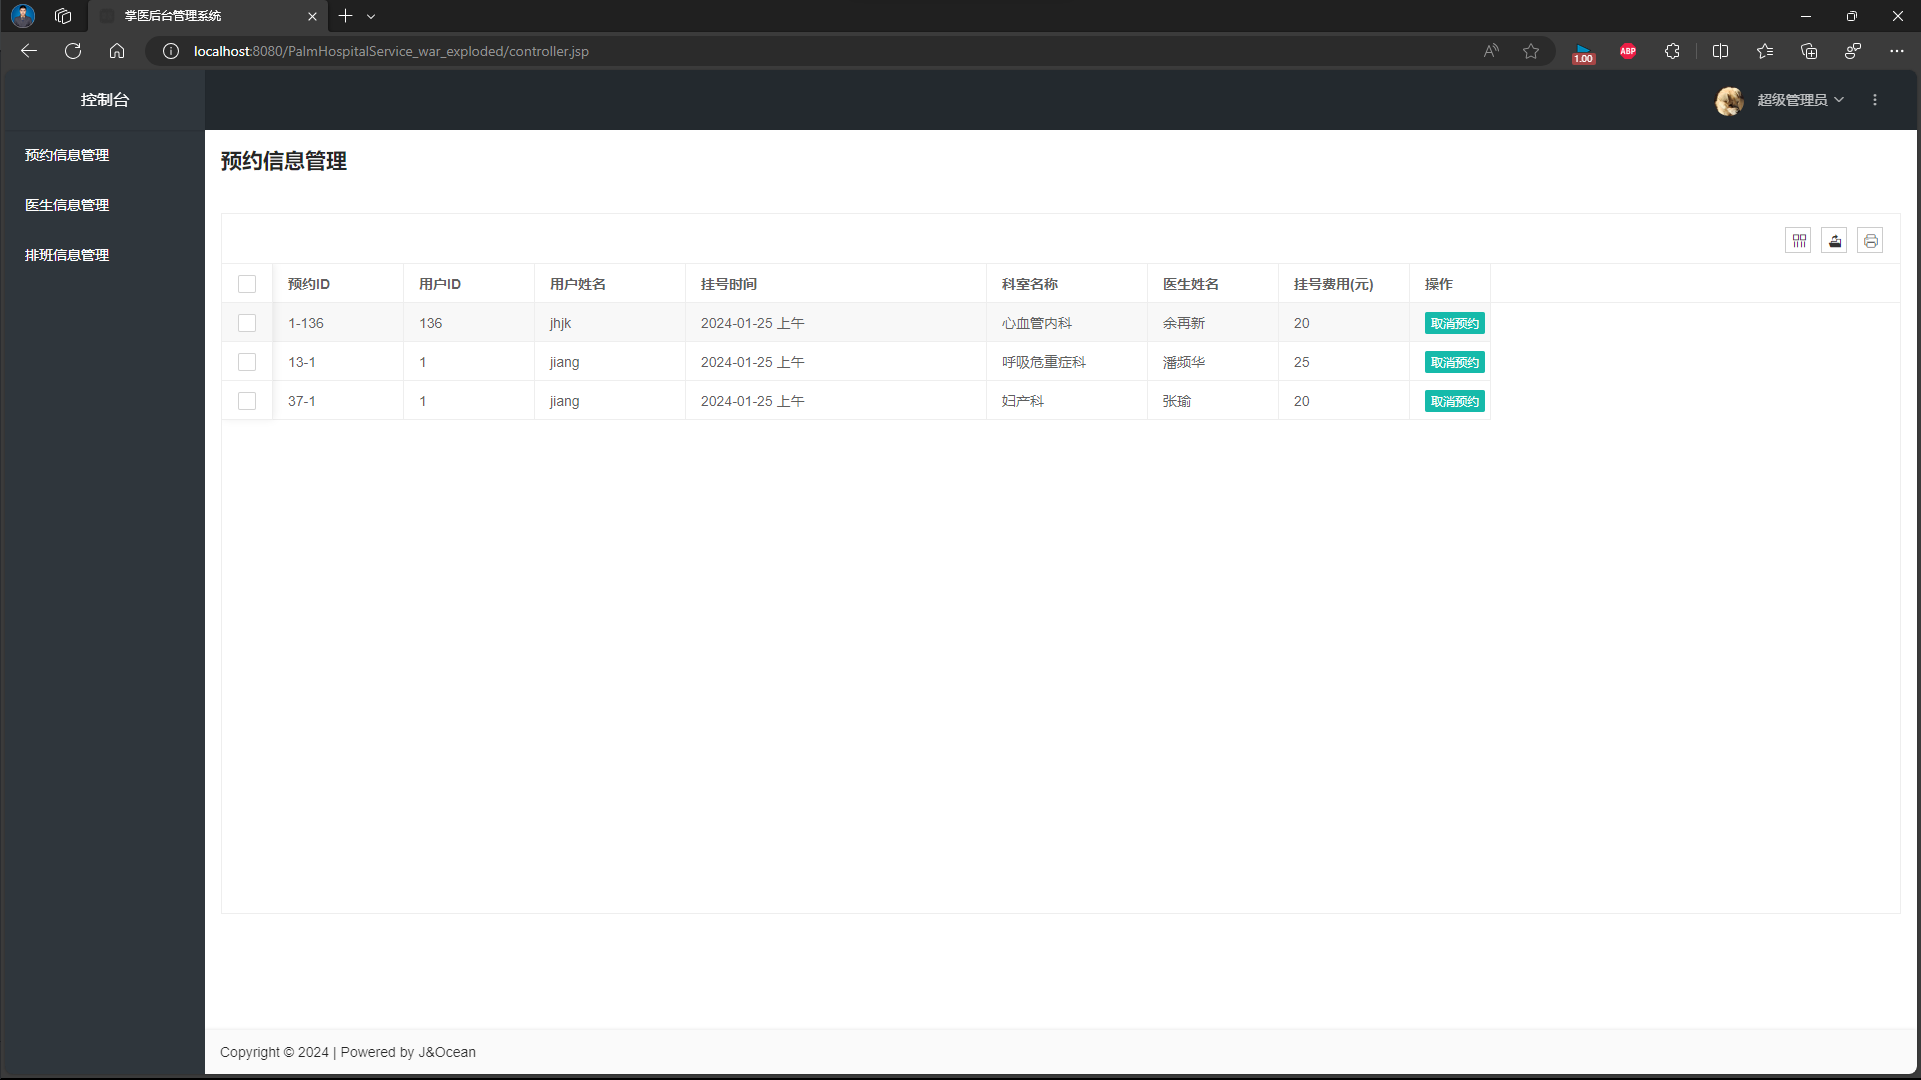
\includegraphics[width=1.0\textwidth]{imgs/17.png}
    \caption{控制台界面}
\end{figure}

控制台界面的设计比较简单,只需要插入三个子页面,使用iframe标签嵌入,对点击时间进行区分,点击不同的按钮,加载不同的页面,实现页面的跳转。

\begin{lstlisting}[frame=shadowbox]
    <ul class="layui-nav layui-nav-tree" lay-filter="test">
        <li class="layui-nav-item layui-nav-itemed">
            <a class="main_left" data-src="orders.jsp">预约信息管理</a>
        </li>

        <li class="layui-nav-item layui-nav-itemed">
            <a class="main_left" data-src="doctors.jsp">医生信息管理</a>
        </li>

        <li class="layui-nav-item layui-nav-itemed">
            <a class="main_left" data-src="schedules.jsp">排班信息管理</a>
        </li>
    </ul>

    ...

    <iframe id="mainframe" frameborder="0" scrolling="yes" style="width: 100%;height: 100%" src="orders.jsp"> </iframe>

    ... 

    <script>
    $(function(){
        $(".main_left").click(function(){
            var src = $(this).attr("data-src");
            $("#mainframe").attr("src",src);
        });
    });
    </script>
\end{lstlisting}

\subsubsection{orders.jsp}
在挂号预约信息界面,需要展示所有的预约信息,包括预约id,用户id,用户姓名,科室名称,医生姓名,预约时间,挂号费等字段,同时需要提供删除预约信息的功能。

\begin{figure}[htbp]
    \centering
    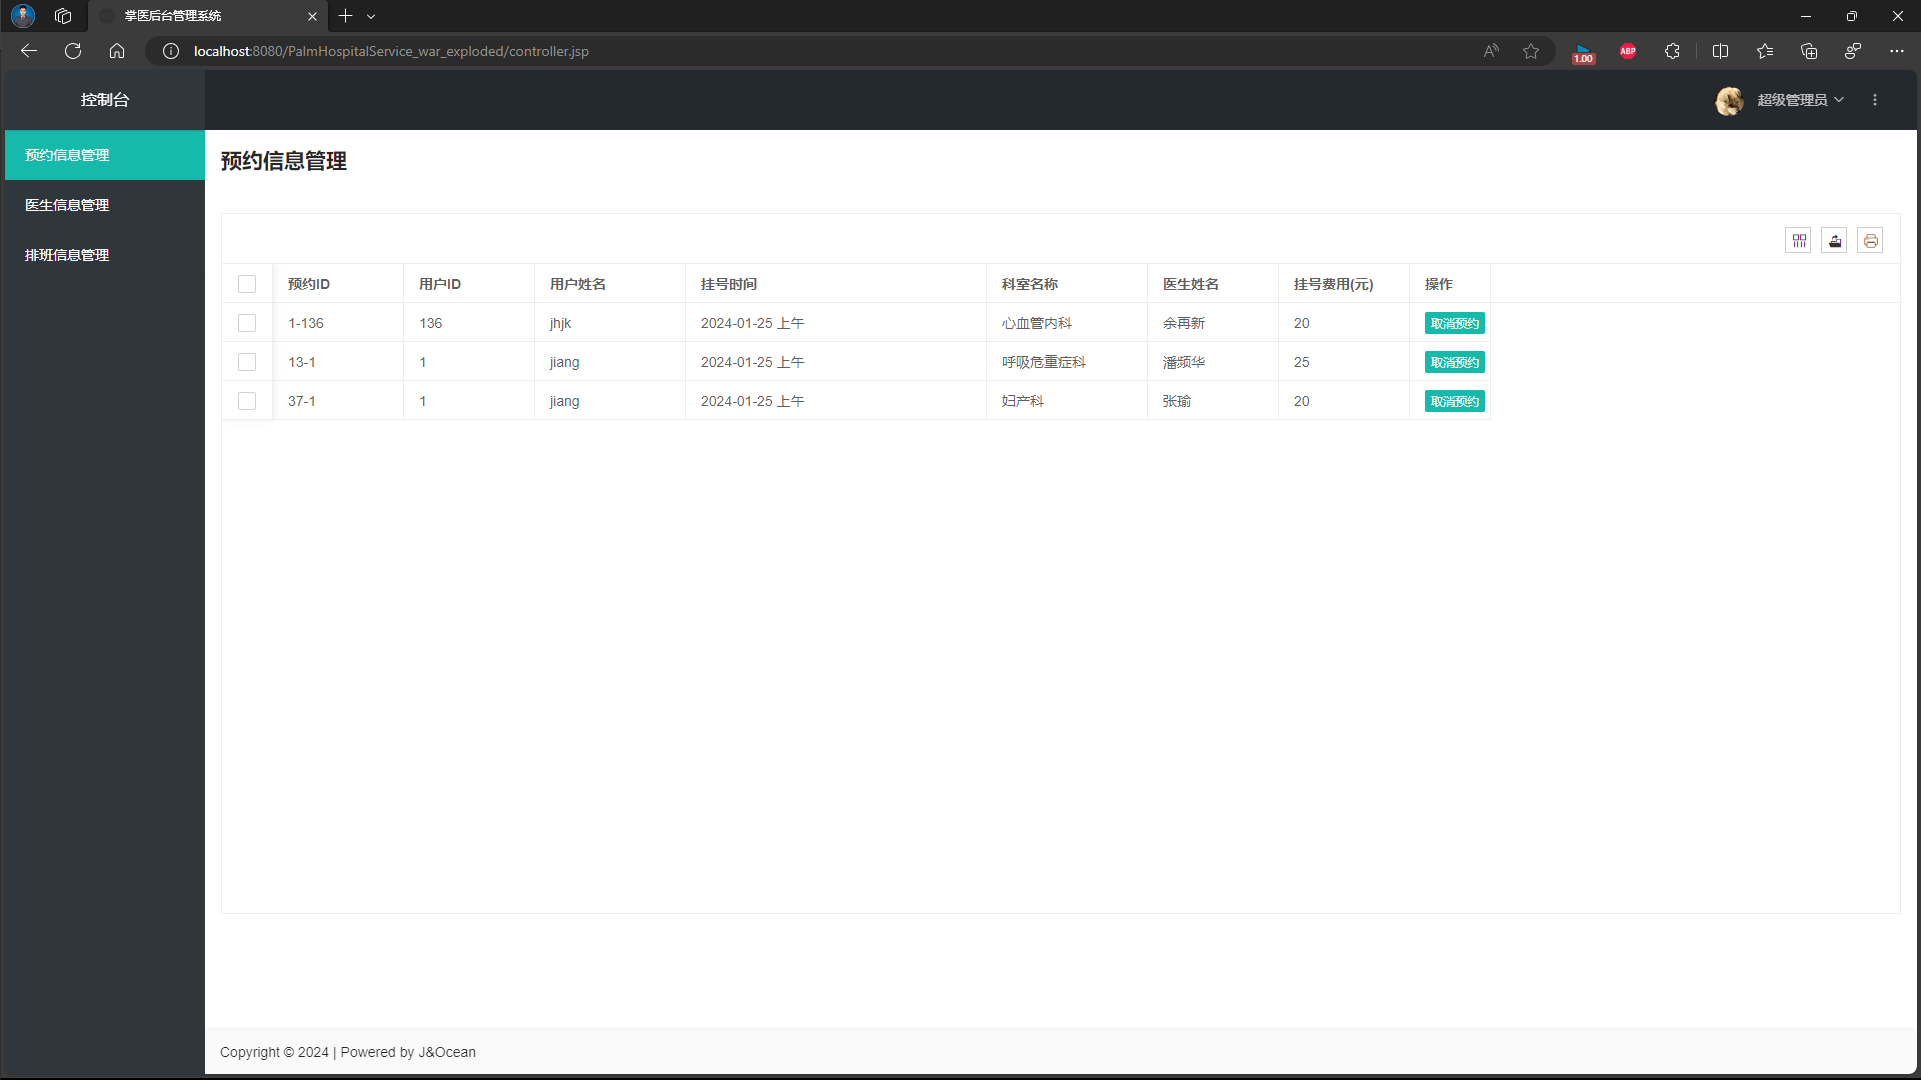
\includegraphics[width=1.0\textwidth]{imgs/18.png}
    \caption{预约信息管理界面}
\end{figure}

表格数据实时动态渲染,使用layui的table模块,具体代码如下:

\begin{lstlisting}[frame=shadowbox]
    table.render({
            elem: '#test',
            url: 'http://localhost:8080/PalmHospitalService_war_exploded/OrderServlet', // 此处为静态模拟数据,实际使用时需换成真实接口
            toolbar: '#toolbarDemo',
            height: 'full-200', // 最大高度减去其他容器已占有的高度差
            css: [ // 重设当前表格样式
                '.layui-table-tool-temp{padding-right: 1000px;}'
            ].join(''),
            cellMinWidth: 80,
            totalRow: false, // 开启合计行
            page: false,
            cols: [[
                {type: 'checkbox', fixed: 'left'},
                {field:'oid',width:130, title: '预约ID'},
                {field:'uid',width:130, title: '用户ID'},
                {field:'uname',width:150, title: '用户姓名'},
                {field:'time',width:300, title: '挂号时间'},
                {field:'departname',width:160, title: '科室名称'},
                {field:'dname',width:130, title: '医生姓名'},
                {field:'price',width:130, title: '挂号费用(元)'},
                {fixed: 'right', title:'操作', width: 80, minWidth: 80, toolbar: '#barDemo'}
            ]],

            ...

            error: function(res, msg){
                console.log(res, msg)
            }
        });
\end{lstlisting}

在前端界面中,对于删除处理的操作,layui原生框架提供了类似操作的封装,对表格的toolbar进行设置,即可实现删除操作,具体代码如下:

\begin{lstlisting}[frame=shadowbox]
    table.on('tool(test)', function(obj){ // 双击 toolDouble
            var data = obj.data; // 获得当前行数据
            console.log(data)
            if(obj.event === 'delete'){
                layer.confirm('确定取消预约 [预约ID: '+ data.oid +'] ', function(index){
                    const url1 = "http://localhost:8080/PalmHospitalService_war_exploded/DeleteOrdersServlet?oid=" + data.oid;
                    // 使用 Fetch API 发起 DELETE 请求
                    fetch(url1, {
                        method: 'GET',
                    })
                        .then(response => {
                            if (!response.ok) {
                                throw new Error('Network response was not ok');
                            }
                        })
                        .then(() => {
                            obj.del(); // 删除对应行(tr)的DOM结构
                        })
                        .catch(error => {
                            // 请求失败时的处理
                            console.error('There has been a problem with your fetch operation:', error);
                        });

                    // obj.del();
                    layer.close(index);
                    // 向服务端发送删除指令
                })
            }
        });
\end{lstlisting}

\newpage

\subsubsection{doctors.jsp}
在医生信息管理界面,需要展示所有的医生信息,包括医生id,医生姓名,医生职级,医生简介,医生详细信息,科室id,科室名称,医生性别等字段,同时需要提供修改医生信息的功能。

\begin{figure}[htbp]
    \centering
    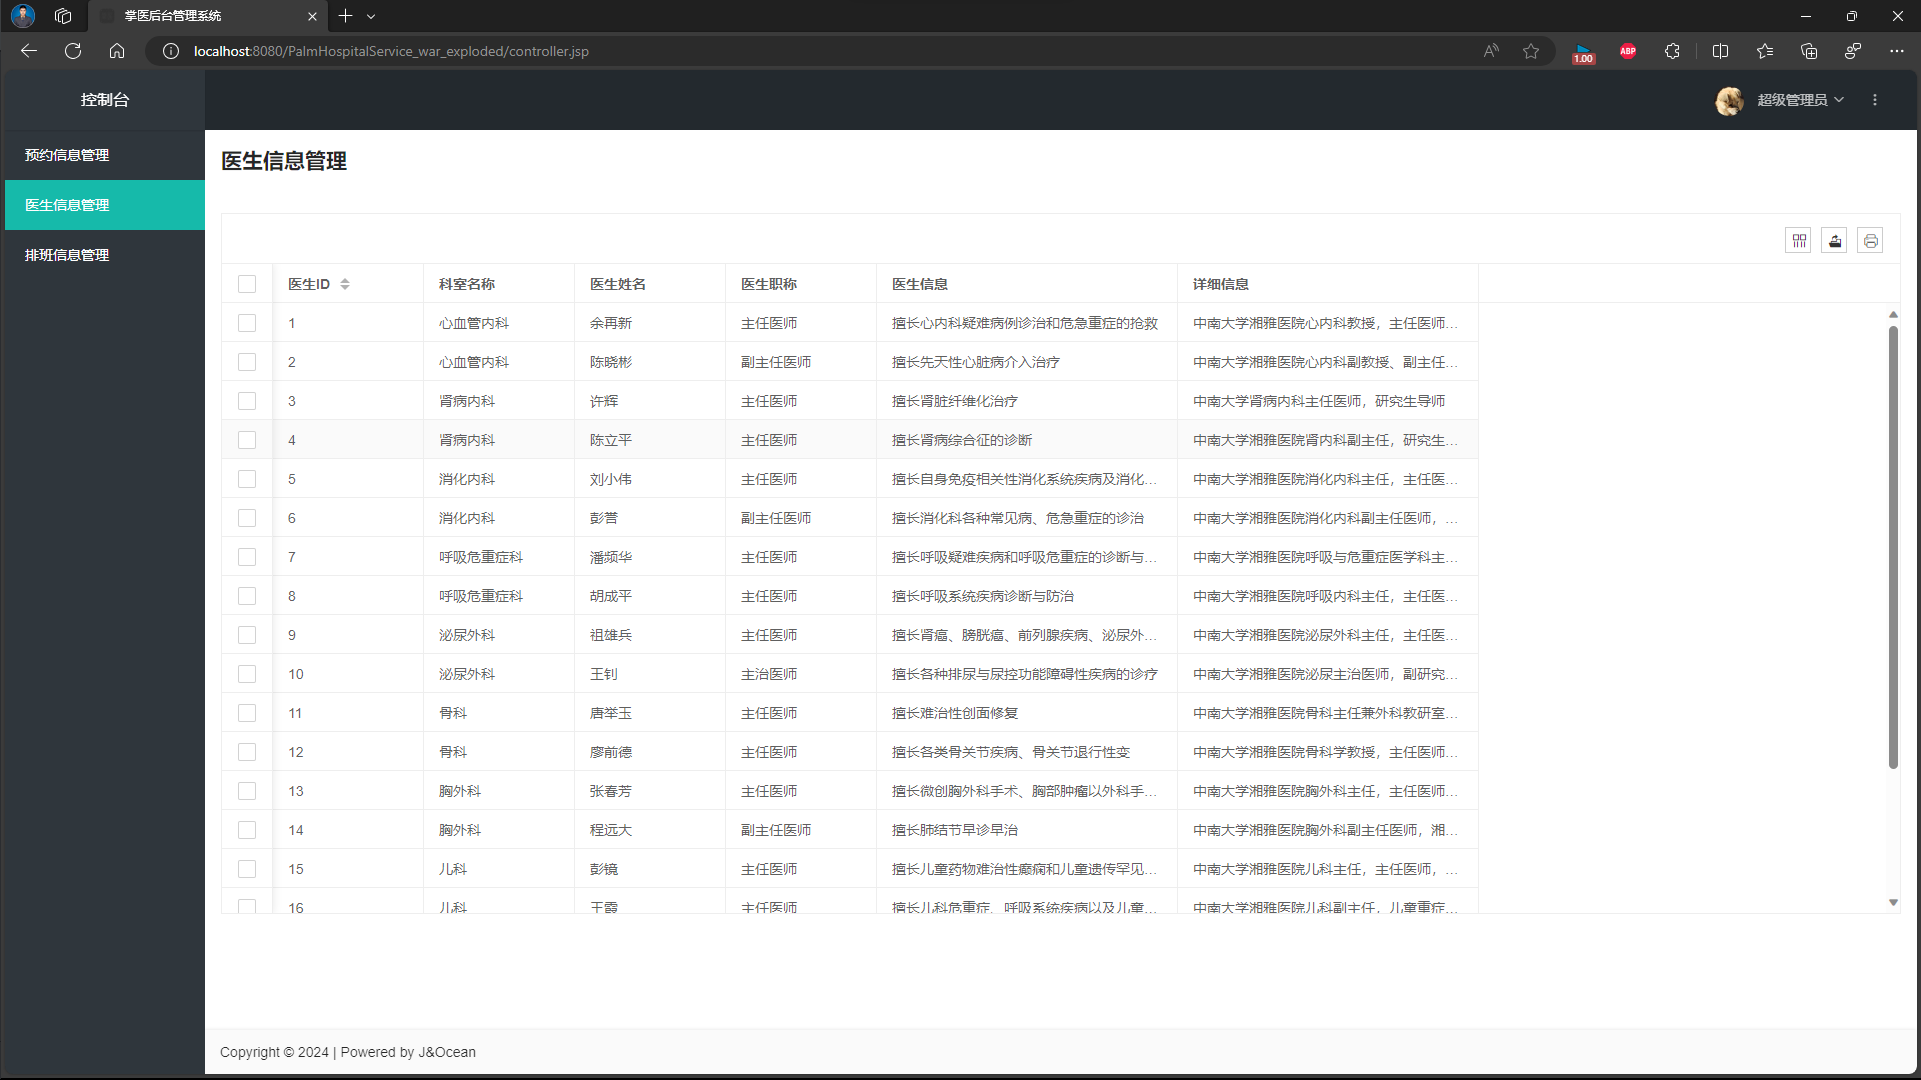
\includegraphics[width=1.0\textwidth]{imgs/19.png}
    \caption{医生信息管理界面}
\end{figure}

表格数据试试动态渲染,使用layui的table模块;修改医生信息设置信息列的edit值为textarea,修改部分使用js实现,与上面的类似,这里不再赘述。

\begin{lstlisting}[frame=shadowbox]
    table.render({...
      url: 'http://localhost:8080/PalmHospitalService_war_exploded/DoctorServlet', // 此处为静态模拟数据,实际使用时需换成真实接口
      ...
      cols: [[{type: 'checkbox', fixed: 'left'},
        {field:'did',width:150, title: '医生ID',sort:true},
        {field:'departname',width:150, title: '科室名称'},
        {field:'dname',width:150, title: '医生姓名'},
        {field:'dlevel',width:150, title: '医生职称'},
        {field:'dinfo', title: '医生信息',width:300,edit: 'textarea'},
        {field:'ddetail',width:300, title: '详细信息',edit: 'textarea'},]],
        ...
    });
\end{lstlisting}

\newpage

\subsubsection{schedules.jsp}

在排班信息管理界面,需要展示所有的排班信息,包括排班id,医生id,排班时间,挂号费等字段,同时需要提供删除排班信息的功能,与预约信息管理界面类似。

\begin{figure}[htbp]
    \centering
    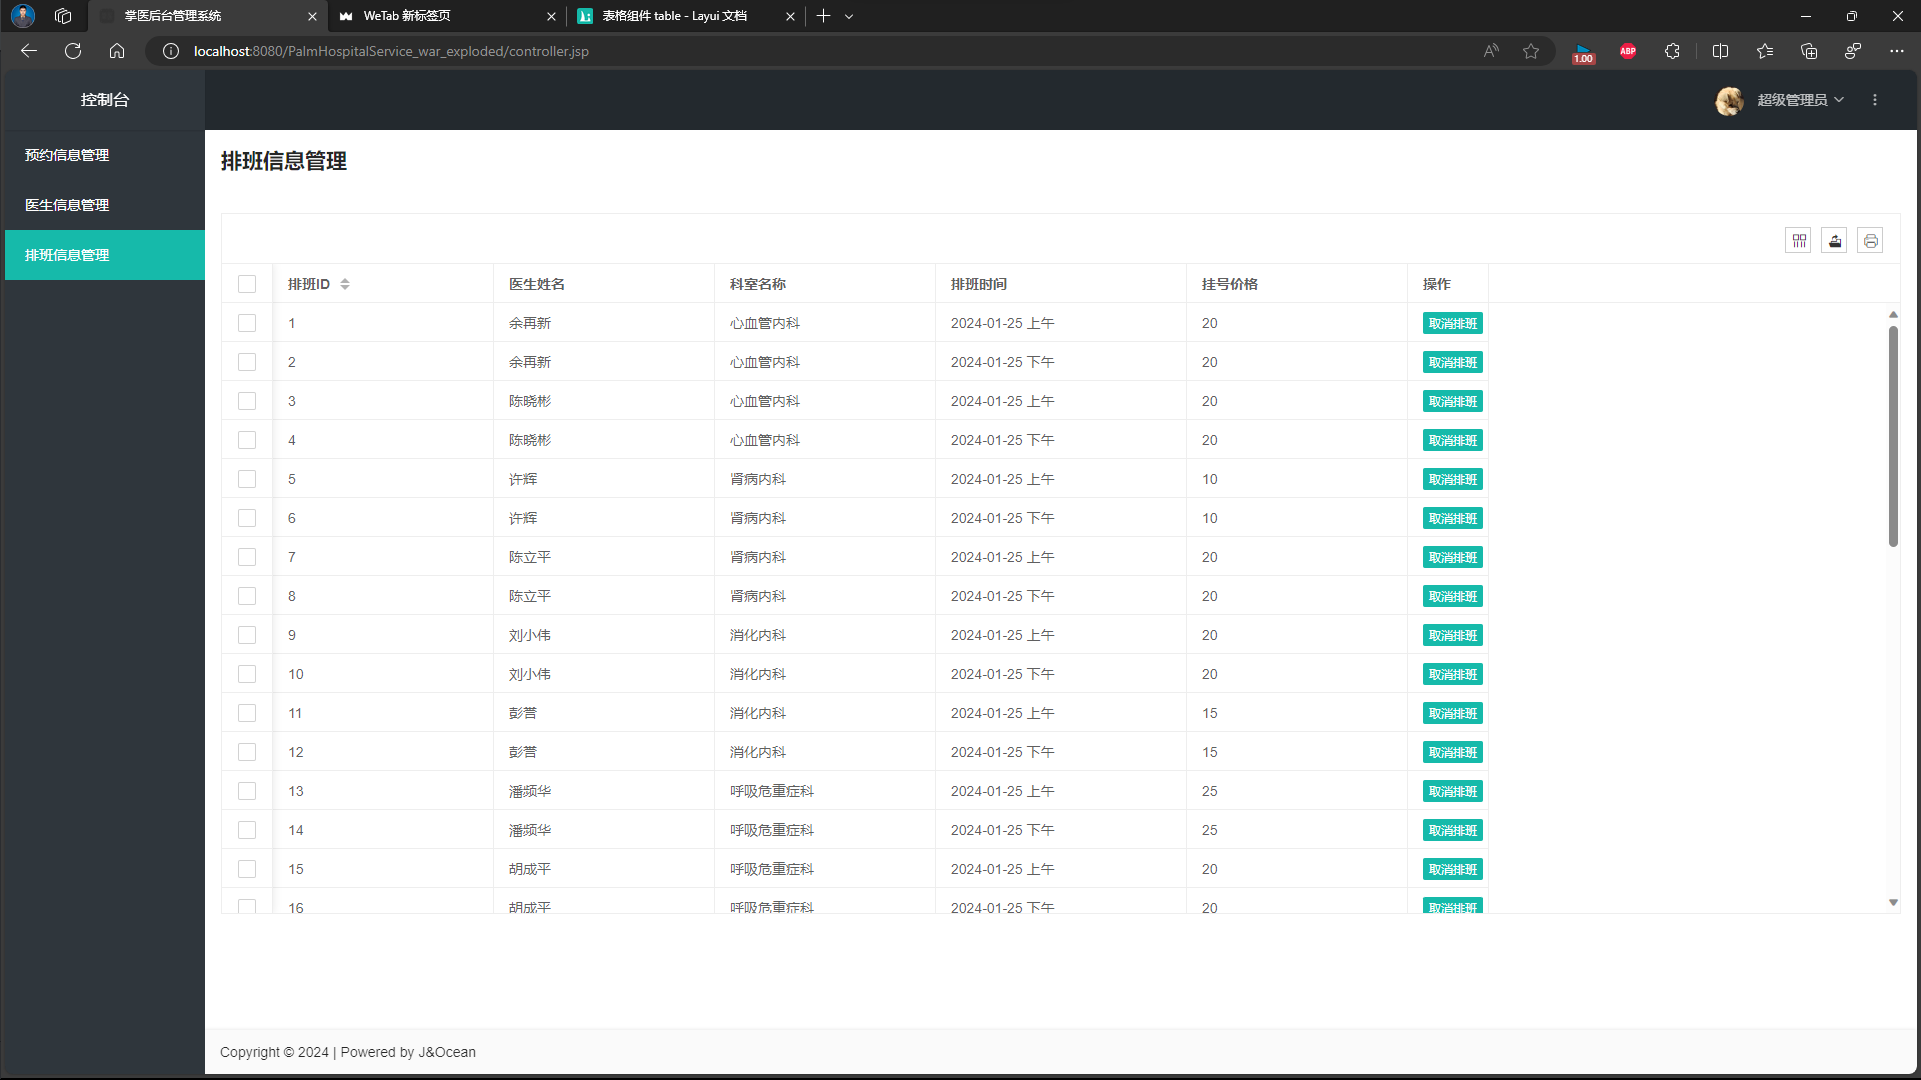
\includegraphics[width=1.0\textwidth]{imgs/20.png}
    \caption{排班信息管理界面}
\end{figure}

\begin{lstlisting}[frame=shadowbox]
    table.render({...
      url: 'http://localhost:8080/PalmHospitalService_war_exploded/ScheduleServlet', // 此处为静态模拟数据,实际使用时需换成真实接口
      ...
      cols: [[
        {type: 'checkbox', fixed: 'left'},
        {field:'sid',width:220, title: '排班ID', sort:true},
        {field:'dname',width:220, title: '医生姓名'},
        {field:'departname',width:220, title: '科室名称'},
        {field:'time',width:250, title: '排班时间'},
        {field:'price', title: '挂号价格',width:220},
        {fixed: 'right', title:'操作', width: 80, minWidth: 80, toolbar: '#barDemo'}
      ]],
      ...
    });
\end{lstlisting}

\newpage

\subsection{预约挂号Web服务器详细设计}
Web服务器需要处理两类业务,一类是移动端的业务,一类是后台管理的业务。那么对于上述业务,我们需要设计的包如下,设置两个包分别处理移动端和后台管理的业务。

\begin{figure}[htbp]
    \centering
    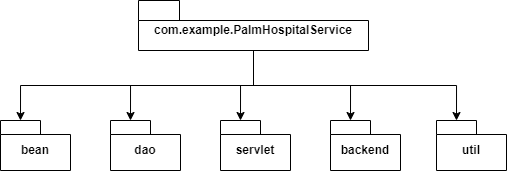
\includegraphics[width=1.0\textwidth]{imgs/16.png}
    \caption{包结构}
\end{figure}

\subsubsection{bean}
包bean用于存放实体类,包括用户、医生、科室、排班、订单等实体类,其中一部分与数据库中单表的结构一致,另一部分是为了方便处理业务而设计的。

包bean包含以下实体类:

\begin{itemize}
    \item Administrator:管理员实体类,包含管理员用户名,密码等字段
    \item BackDoctors:后端医生实体类,包含医生id,医生姓名,医生职级,医生简介,医生详细信息等字段
    \item BackOrders:后端预约实体类,包含预约id,用户id,用户姓名,科室名称,医生姓名,预约时间,挂号费等字段
    \item BackSchedules:后端排班实体类,包含排班id,医生id,排班时间,挂号费等字段
    \item Depart:科室实体类,包含科室id,科室名称等字段
    \item Doctor:医生实体类,包含医生id,医生姓名,医生职级,医生简介,医生详细信息,科室id,科室名称,医生性别等字段
    \item Order/Orders:两个不同用途的预约实体类
    \item Schedule:排班实体类,包含排班id,医生id,排班时间,挂号费等字段
    \item User:用户实体类,包含用户id,用户名,密码
\end{itemize}

\subsubsection{dao}
包dao用于存放数据访问对象,包括用户、医生、科室、排班、订单等数据访问对象,其中一部分与数据库中单表的结构一致,另一部分是为了方便处理业务而设计的。

包dao包含以下数据访问对象:

\begin{itemize}
    \item AdministratorDao:管理员数据访问对象,包含管理员用户名,密码等字段
    \item BackDoctorsDao:后端医生数据访问对象,包含医生id,医生姓名,医生职级,医生简介,医生详细信息等字段
    \item BackOrderDao:后端预约数据访问对象,包含预约id,用户id,用户姓名,科室名称,医生姓名,预约时间,挂号费等字段
    \item BackSchedulesDao:后端排班数据访问对象,包含排班id,医生id,排班时间,挂号费等字段
    \item DepartDao:科室数据访问对象,包含科室id,科室名称等字段
    \item DoctorDao:医生数据访问对象,包含医生id,医生姓名,医生职级,医生简介,医生详细信息,科室id,科室名称,医生性别等字段
    \item OrderDao:预约数据访问对象,包含预约id,用户id,用户姓名,科室名称,医生姓名,预约时间,挂号费等字段
    \item ScheduleDao:排班数据访问对象,包含排班id,医生id,排班时间,挂号费等字段
    \item UserDao:用户数据访问对象,包含用户id,用户名,密码
\end{itemize}

\subsubsection{Servlet}
包Servlet用于存放移动端数据请求处理的Servlet,包括用户、医生、科室、排班、订单等Servlet

包servlet包含以下servlet对象:

\begin{itemize}
    \item ChooseDepartServlet:选择科室Servlet,用于处理移动端选择科室的请求
    \item ChooseDoctorServlet:选择医生Servlet,用于处理移动端选择医生的请求
    \item ChooseTimeServlet:选择时间Servlet,用于处理移动端选择时间的请求
    \item LoginServlet:登录Servlet,用于处理移动端登录的请求
    \item MyInfoServlet:我的信息Servlet,用于处理移动端我的信息的请求
    \item PayServlet:支付Servlet,用于处理移动端支付的请求
    \item RegisterServlet:注册Servlet,用于处理移动端注册的请求
\end{itemize}

\subsubsection{backend}
包backend用于存放后台管理数据请求处理的Servlet,包括用户、医生、科室、排班、订单等Servlet

包backend包含以下servlet对象:

\begin{itemize}
    \item BackRegisterServlet:后台管理注册Servlet,用于处理后台管理注册的请求
    \item DeleteOrdersServlet: 删除预约Servlet,用于处理后台管理删除预约的请求
    \item DeleteSchedulesServlet:删除排班Servlet,用于处理后台管理删除排班的请求
    \item DoctorServlet: 医生Servlet,用于处理后台管理医生的请求
    \item LogoutServlet:注销Servlet,用于处理后台管理注销的请求
    \item OrderServlet:预约Servlet,用于处理后台管理预约的请求
    \item ScheduleServlet:排班Servlet,用于处理后台管理排班的请求
    \item TestServlet: 登录Servlet,用于登录,由于一开始在该class上测试及运行故没有更改名字
\end{itemize}

bean包中的实体类定义了各个实体类的属性,并定义了相应的get和set方法,定义了重载的构造方法,用于初始化实体类对象。

\begin{lstlisting}[frame=shadowbox]

public class ABC {
    
    private String XXX;
    private String YYY;
    private String ZZZ;

    public ABC() {

    }

    public ABC(String XXX, String YYY, String ZZZ) {
        this.XXX = XXX;
        this.YYY = YYY;
        this.ZZZ = ZZZ;
    }

    public String getXXX() {
        return XXX;
    }

    public void setXXX(String XXX) {
        this.XXX = XXX;
    }

    public String getYYY() {
        return YYY;
    }

    public void setYYY(String YYY) {
        this.YYY = YYY;
    }

    public String getZZZ() {
        return ZZZ;
    }

    public void setZZZ(String ZZZ) {
        this.ZZZ = ZZZ;
    }
}

\end{lstlisting}

dao包中的数据访问对象定义了各个实体类的增删改查方法,用于对数据库进行操作,以管理员数据访问对象AdministratorDao为例:

\begin{lstlisting}[frame=shadowbox]
public class AdministratorDao {
    private QueryRunner queryRunner = new QueryRunner();

    public Administrator selectAdministratorByUser(String user){
        Administrator administrator=null;
        try{
            administrator=queryRunner.query(DbUtil.getConnection(),"select * from administrator " +
                    "where administrator.user=?;",new BeanHandler<Administrator>(Administrator.class),user);
        }catch(SQLException e){
            e.printStackTrace();
        }
        return administrator;
    }

    public int AddAdministrator(Administrator administrator){
        int res=0;
        try{
            res=queryRunner.update(DbUtil.getConnection(),"insert into administrator values(?,?)",administrator.getUser(),administrator.getPassword());
        }catch(SQLException e){
            e.printStackTrace();
        }
        return res;
    }
}
\end{lstlisting}

dao的核心语句在于SQL语句编写,然后调用Dbutil方法连接MySQL数据库,然后调用QueryRunner方法执行SQL语句,最后返回结果。

\begin{lstlisting}[frame=shadowbox]
public class XXXDao{
    private QueryRunner queryRunner = new QueryRunner();

    public XXX selectXXXByXXX(String XXX){
        XXX XXX=null;
        try{
            XXX=queryRunner.query(DbUtil.getConnection(),"select * from XXX " +
                    "where XXX.XXX=?;",new BeanHandler<XXX>(XXX.class),XXX);
        }catch(SQLException e){
            e.printStackTrace();
        }
        return XXX;
    }

    public int AddXXX(XXX XXX){
        int res=0;
        try{
            res=queryRunner.update(DbUtil.getConnection(),"insert into XXX values(?,?,?)",XXX.getXXX(),XXX.getYYY(),XXX.getZZZ());
        }catch(SQLException e){
            e.printStackTrace();
        }
        return res;
    }
}
\end{lstlisting}

servlet/backend包中的servlet类,都继承了HttpServlet类,重写了doGet和doPost方法,用于处理get和post请求,具体的实现方法如下:

\begin{lstlisting}[frame=shadowbox]
@WebServlet(name="XXXServlet",value="/XXXServlet")
public class XXXServlet extends HttpServlet {
    public XXXServlet (){
        super();
    }

    protected void doGet(HttpServletRequest request, HttpServletResponse response) throws IOException {
        // 设置GET方法的响应内容类型
    }


    public void doPost(HttpServletRequest request, HttpServletResponse response) throws ServletException, IOException {
        // 设置POST方法的响应内容类型
        doGet(request, response);
    }
}
\end{lstlisting}



\subsubsection{utils}
里面有用于连接数据库的工具类DBUtil

\begin{lstlisting}[frame=shadowbox]
package com.example.palmhospitalservice.utils;

import com.alibaba.druid.pool.DruidDataSource;
import com.alibaba.druid.pool.DruidDataSourceFactory;
import org.apache.commons.dbutils.DbUtils;

import java.io.IOException;
import java.io.InputStream;
import java.sql.Connection;
import java.sql.ResultSet;
import java.sql.SQLException;
import java.sql.Statement;
import java.util.Properties;

public class DbUtil {
    private static DruidDataSource ds;
    private static final ThreadLocal<Connection> THREAD_LOCAL = new ThreadLocal<>();

    static {
        Properties properties = new Properties();
        InputStream inputStream = DbUtils.class.getResourceAsStream("/database.properties");
        try {
            properties.load(inputStream);
            ds = (DruidDataSource) DruidDataSourceFactory.createDataSource(properties);
        } catch (IOException e) {
            e.printStackTrace();
        } catch (Exception e) {
            e.printStackTrace();
        }

    }
    public static Connection getConnection() {

        Connection connection = THREAD_LOCAL.get();

        try {
            if (connection == null) {
                connection = ds.getConnection();

                THREAD_LOCAL.set(connection);
            }
        } catch (SQLException e) {
            e.printStackTrace();
        }


        return connection;
    }
    public static void begin() {
        Connection connection = null;
        connection = getConnection();
        try {
            connection.setAutoCommit(false);
        } catch (SQLException e) {
            e.printStackTrace();
        }
    }
    public static void commit() {
        Connection connection = null;
        try {
            connection = getConnection();
            connection.commit();
        } catch (SQLException e) {
            e.printStackTrace();
        } finally {
            closeAll(connection, null, null);
        }
    }
    public static void rollback() {
        Connection connection = null;
        try {
            connection = getConnection();
            connection.rollback();
        } catch (SQLException e) {
            e.printStackTrace();
        } finally {
            closeAll(connection, null, null);
        }
    }
    public static void closeAll(Connection connection, Statement statement, ResultSet resultSet) {
        try {
            if (resultSet != null) {
                resultSet.close();
            }
            if (statement != null) {
                statement.close();
            }
            if (connection != null) {
                connection.close();
                THREAD_LOCAL.remove();
            }
        } catch (SQLException e) {
            e.printStackTrace();
        }
    }
}
\end{lstlisting}

\newpage

\section{调试方法}

\subsection{移动端调试方法}

\subsubsection{Android端连接服务器失败}
Android端build之后,应用正常启动,但是在登录的时候,提示账号密码错误,查看Logcat,发现如下错误:

\begin{figure}[htbp]
    \centering
    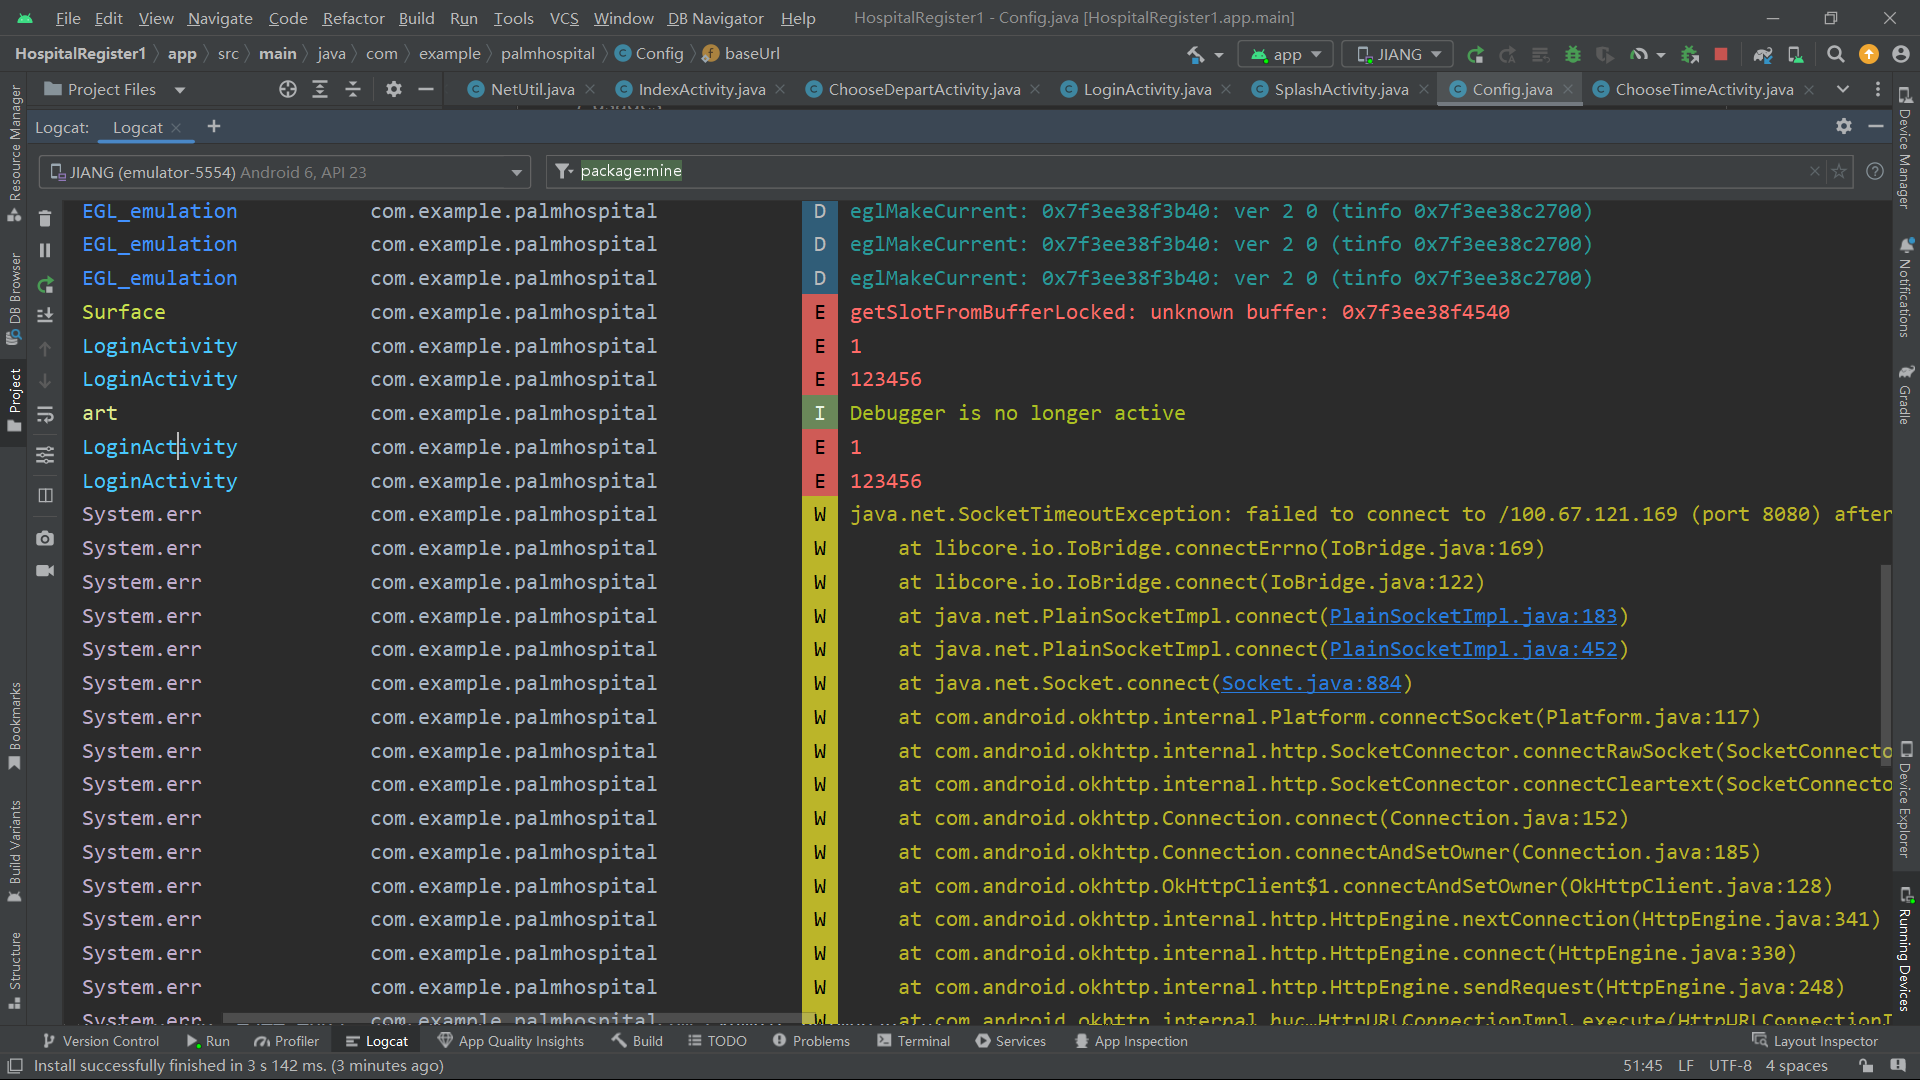
\includegraphics[width=1.0\textwidth]{imgs/27.png}
    \caption{Android端连接服务器失败}
\end{figure}

\begin{lstlisting}[frame=shadowbox]
    java.net.SocketTimeoutException: failed to connect to /100.67.121.169 (port 8080) after 30000ms
\end{lstlisting}

报错指向的是虚拟机没有办法访问服务器的ip地址,同时地址不能使用127.0.0.1,因为127.0.0.1是虚拟机本身的地址,而不是主机的地址。

原因是由于开发者电脑连接的是校园网Wifi,而不是有线的Ethernet,导致本机的ip地址发生了变化,因此需要修改Config类中的baseUrl,将ip地址修改为当前电脑的ip地址,然后重新build,即可解决问题。

在cmd中输入ipconfig,查看本机的ip地址,如下图所示:

\newpage

\begin{figure}[htbp]
    \centering
    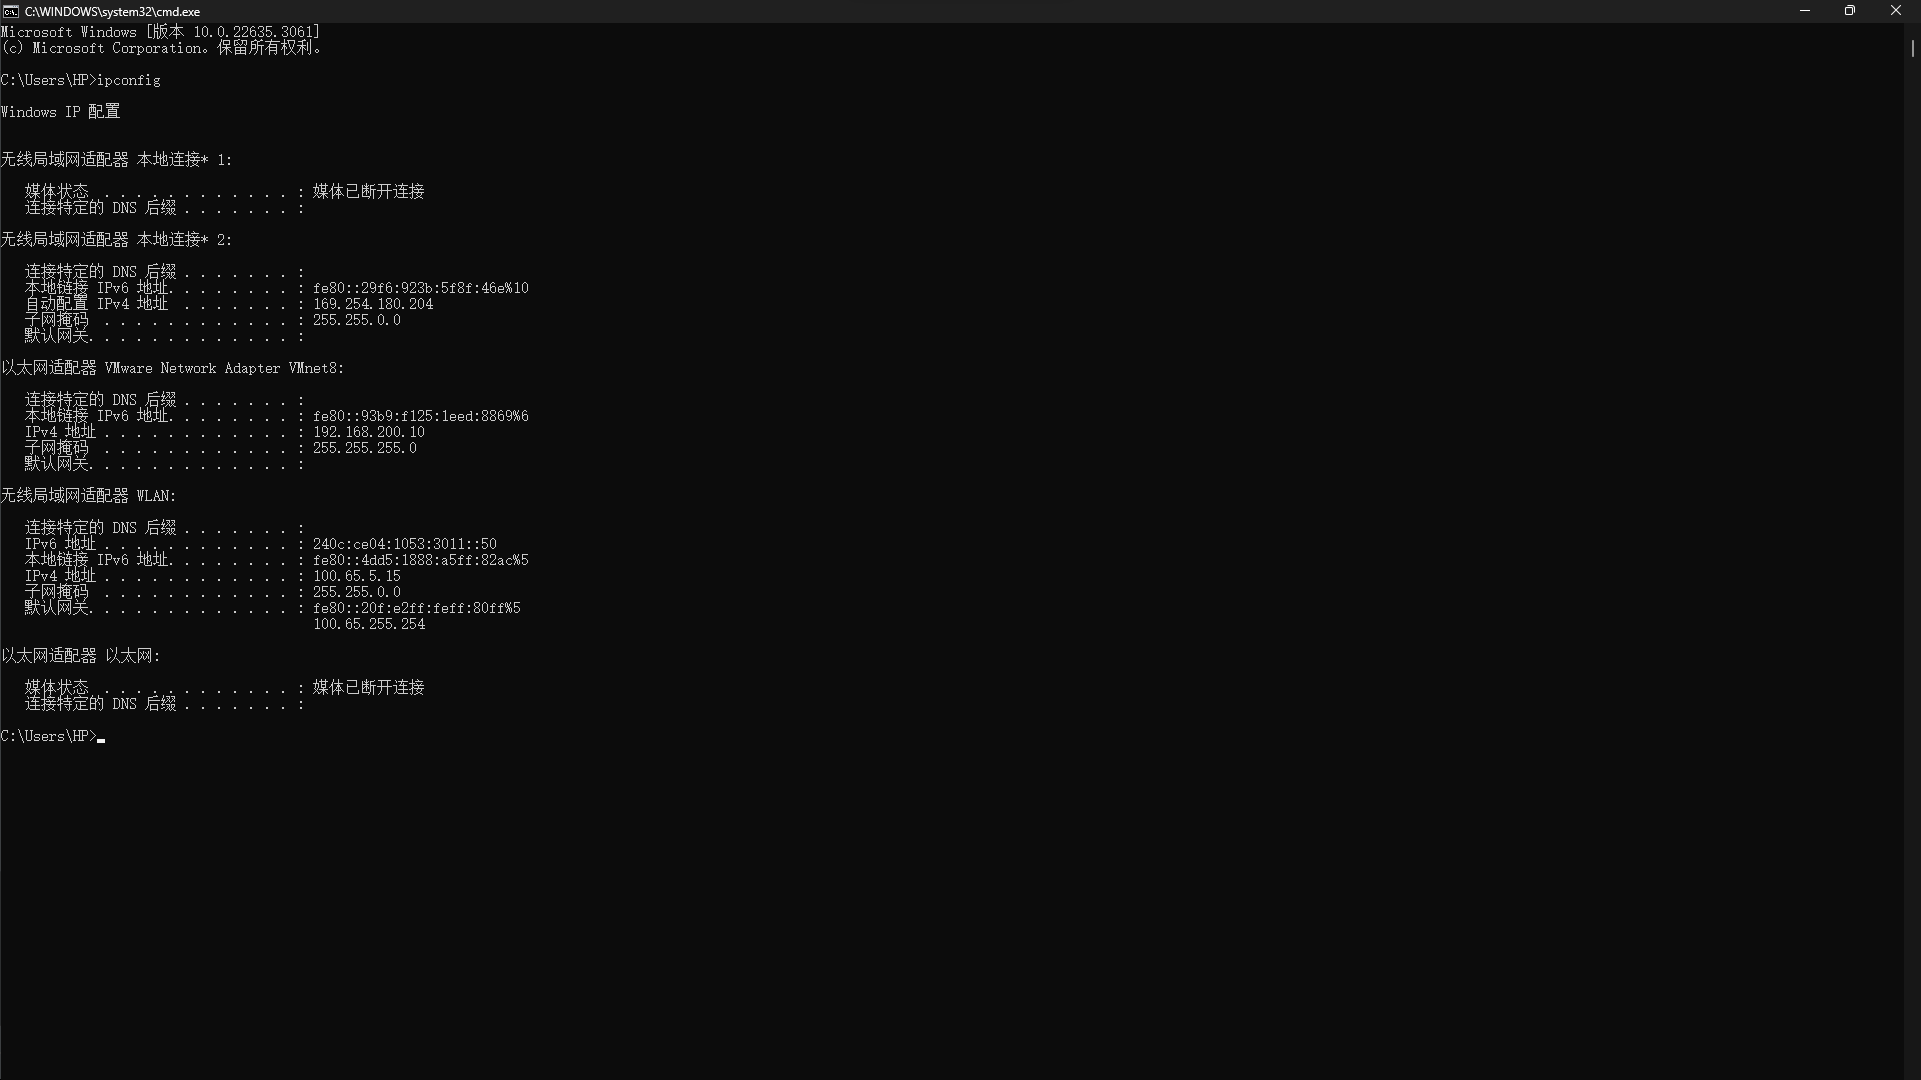
\includegraphics[width=1.0\textwidth]{imgs/28.png}
    \caption{查看本机ip地址}
\end{figure}

在Config.java中修改baseUrl,将ip地址修改为当前主机的ip地址

\begin{lstlisting}[frame=shadowbox]
public class Config {
    public static String baseUrl ="http://100.65.5.15:8080/PalmHospitalService_war_exploded/";
}
\end{lstlisting}

启动服务器后再重新编译运行Android端,即可解决问题。

\subsubsection{Android端连接服务器成功,但是无法获取数据}

Android端build之后,应用正常启动,但是在登录的时候,提示账号密码错误,查看Logcat,发现传递参数无误,因此将错误定位在服务器端,查看Servlet的方法

\begin{lstlisting}[frame=shadowbox]
    package com.example.palmhospitalservice.servlet;

    import ...   
    
    public class LoginServlet extends HttpServlet {
        ...
    }
\end{lstlisting}

可以看到LoginServlet方法没有WebServlet注解,因此无法被访问,需要添加WebServlet注解,修改后的代码如下:

\begin{lstlisting}[frame=shadowbox]
    package com.example.palmhospitalservice.servlet;

    import ...   
    
    @WebServlet(name = "LoginServlet", value = "/LoginServlet")
    public class LoginServlet extends HttpServlet {
        ...
    }
\end{lstlisting}

Servlet API 3.0 引入了一个名为javax.servlet.annotation的新包,
它提供了可用于注释 servlet 类的注释类型。
注释可以替换 Web 部署描述符文件 ( web.xml ) 中的等效 XML 配置,
例如 servlet 声明和 servlet 映射。
Servlet 容器将在部署时处理带注释的类。
注解@WebServlet用于声明一个servlet 类(该类仍然必须从HttpServlet类扩展)并为其配置映射,
可以不用在web.xml里面配置servlet,只需要加上@WebServlet注解就可以修改该servlet的属性了。
web.xml可以配置的servlet属性,在@WebServlet中都可以配置。

\subsection{服务器端调试方法}
\subsubsection{登录判断字符串为空}
直接使用uid==null||upsw==null判断字符串为空,但是发现判断不成功,因此更改逻辑,在UserDao中进行select操作,如果返回的User对象为空,则说明用户名或密码错误,否则登录成功。

\begin{lstlisting}[frame=shadowbox]
    //UserDao
    ...
    public User select(String uid) {
        User user = new User();
        try {
            user = queryRunner.query(DbUtil.getConnection(),"select * from user where uid=?",new BeanHandler<User>(User.class),uid);

        } catch (SQLException e) {
            e.printStackTrace();
        }
        return user;
    }
    ...
    //LoginServlet
    ...
    UserDao userDao = new UserDao();
    User user = userDao.login(uid,upsw);

    PrintWriter writer=response.getWriter();
    String result="";

    if(user == null){   // 登录失败
        response.setStatus(HttpServletResponse.SC_UNAUTHORIZED);
    }
    else{       // 登录成功
        response.setStatus(HttpServletResponse.SC_OK);
        result= new Gson().toJson(user, User.class);        // 将user的数据变成json格式,传输给客户端
        writer.write(result);
        writer.flush();
        writer.close();
    }
    ...    
\end{lstlisting}

\subsubsection{账号密码的传输安全问题}
在登录的时候,如果使用GET方法,账号密码是以明文的形式传输的,在Servlet网址中就可以直接看到账号密码,因此需要使用POST方法,将账号密码以表单的形式传输,这样账号密码就不会以明文的形式传输,而是以表单的形式传输,这样就可以保证账号密码的安全性。

\begin{lstlisting}[frame=shadowbox]
    protected void doGet(HttpServletRequest request, HttpServletResponse response) throws ServletException, IOException {
        ...
    }
    @Override
    protected void doPost(HttpServletRequest request, HttpServletResponse response) throws ServletException, IOException {
        doGet(request,response);
    }
\end{lstlisting}

\subsection{前端页面调试}
\subsubsection{前端动态渲染表格失败}
在服务器启动的前提下,前端动态渲染表格依旧失败,查看Servlet方法返回数据正常,然而查看layui的表格接口数据文档发现,layui的表格接口数据需要满足以下格式:

\begin{lstlisting}[frame=shadowbox]
    {
        "code": 0,
        "msg": "",
        "count": 1000,
        "data": [{}, {}]
    }
\end{lstlisting}

也就是说,除了数据满足json的键值对格式之外,前面还需要加上code,msg,count等字段,因此需要在Servlet方法中添加这些字段,修改后的代码如下:

\begin{lstlisting}[frame=shadowbox]
    result="{\"code\": 0,\"msg\": \"\",\n" +
                "\"count\": "+ backDoctors.size()+",\n" +
                "\"data\": " + data +"}";
\end{lstlisting}

然而,修改之后依旧无法动态渲染表格,怀疑是请求数据的url除了问题,修改为绝对路径后方解决问题

\begin{lstlisting}[frame=shadowbox]
    url: 'http://localhost:8080/PalmHospitalService_war_exploded/XXXServlet',
\end{lstlisting}

\newpage

\section{测试结果}

\subsection{移动端测试结果}
\subsubsection{启动界面}
在点击移动端应用程序图标后,启动界面如下图所示:

\begin{figure}[htbp]
    \centering
    
\includegraphics[width=0.2\textwidth]{imgs/10.png}
    \caption{启动界面}
\end{figure}

\subsubsection{登录界面}
启动程序之后,进入登录界面,登录失败和登录成功的界面如下图所示:

\begin{figure}[htbp]
    \begin{minipage}[t]{0.45\textwidth}
        \centering
        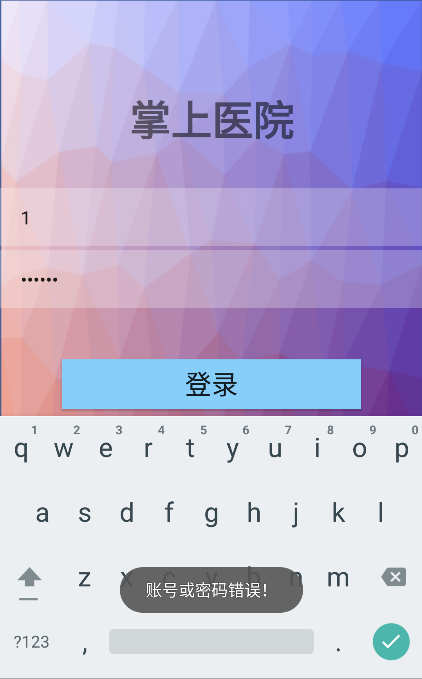
\includegraphics[width=0.7\textwidth]{imgs/29.png}
        \caption{登录失败界面}
    \end{minipage}%
    \begin{minipage}[t]{0.45\textwidth}
        \centering
        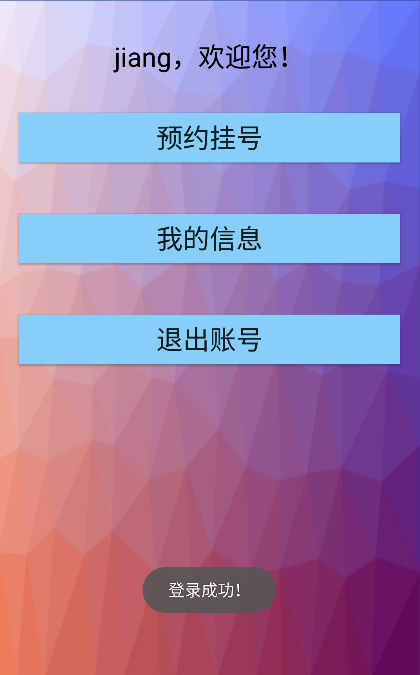
\includegraphics[width=0.7\textwidth]{imgs/30.png}
        \caption{登录成功界面}
    \end{minipage}
\end{figure}

\subsubsection{注册界面}
在登录界面点击注册按钮后,进入注册界面,注册成功和注册失败的界面如下图所示:

\begin{figure}[htbp]
    \begin{minipage}[t]{0.45\textwidth}
        \centering
        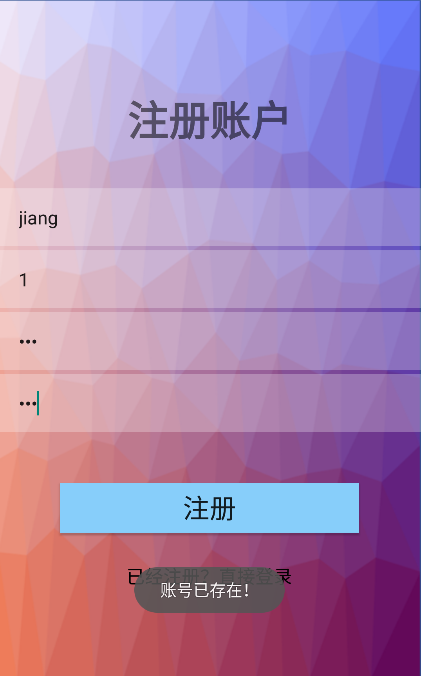
\includegraphics[width=0.7\textwidth]{imgs/32.png}
        \caption{注册失败界面}
    \end{minipage}%
    \begin{minipage}[t]{0.45\textwidth}
        \centering
        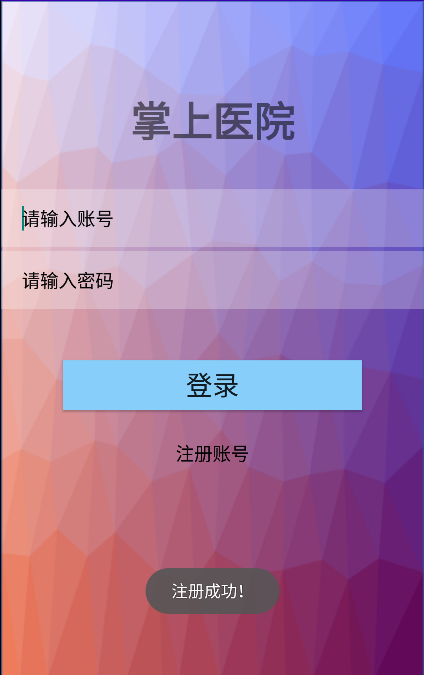
\includegraphics[width=0.7\textwidth]{imgs/31.png}
        \caption{注册成功界面}
    \end{minipage}
\end{figure}

\subsubsection{首页界面}

在登录成功之后,进入首页界面,首页界面如下图所示:

\begin{figure}[htbp]
    \centering
    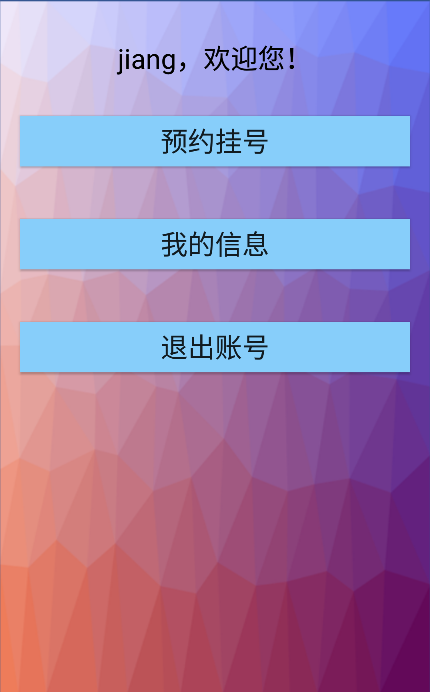
\includegraphics[width=0.25\textwidth]{imgs/13.png}
    \caption{首页界面}
\end{figure}

\newpage

\subsubsection{预约测试}

\begin{figure}[htbp]
    \begin{minipage}[t]{0.45\textwidth}
        \centering
        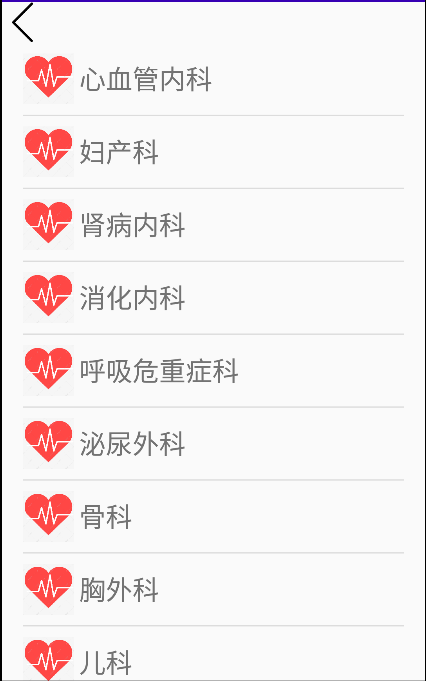
\includegraphics[width=0.6\textwidth]{imgs/21.png}
        \caption{选择科室界面}
    \end{minipage}%
    \begin{minipage}[t]{0.45\textwidth}
        \centering
        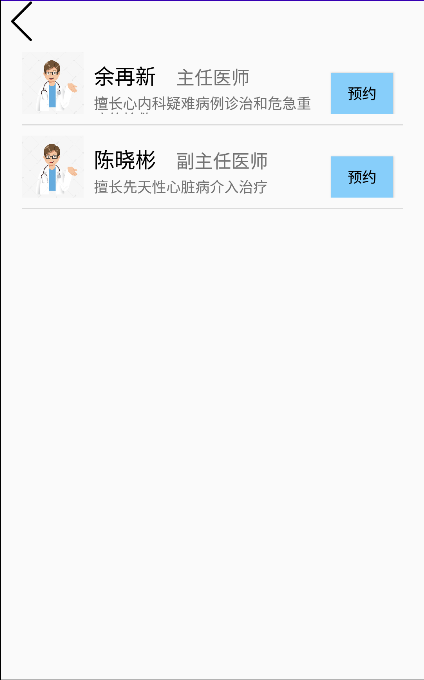
\includegraphics[width=0.6\textwidth]{imgs/22.png}
        \caption{选择医生界面}
    \end{minipage}
\end{figure}

\begin{figure}[htbp]
    \begin{minipage}[t]{0.45\textwidth}
        \centering
        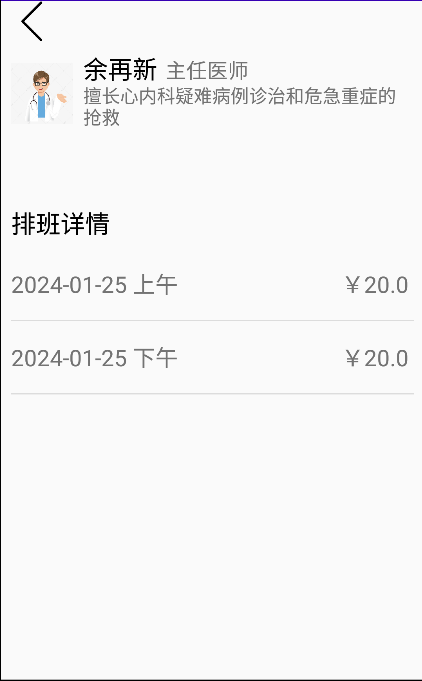
\includegraphics[width=0.6\textwidth]{imgs/24.png}
        \caption{选择时间界面}
    \end{minipage}%
    \begin{minipage}[t]{0.45\textwidth}
        \centering
        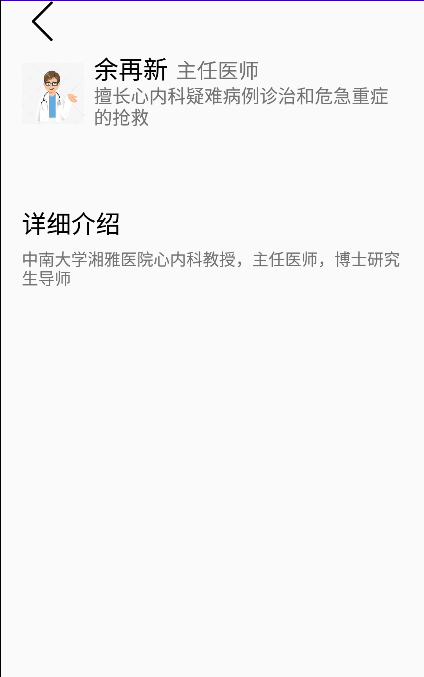
\includegraphics[width=0.6\textwidth]{imgs/23.png}
        \caption{医生详情界面}
    \end{minipage}
\end{figure}

\newpage

\begin{figure}[htbp]
    \centering
    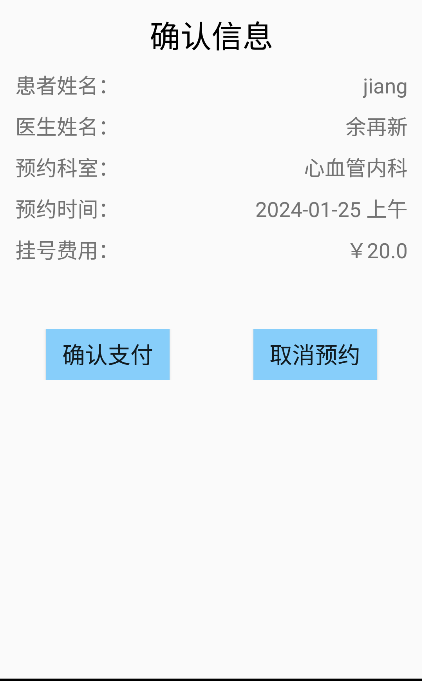
\includegraphics[width=0.25\textwidth]{imgs/25.png}
    \caption{支付界面}
\end{figure}

\subsubsection{我的信息界面}

在首页界面点击我的信息按钮后,进入我的信息界面,我的信息界面如下图所示:

\begin{figure}[htbp]
    \centering
    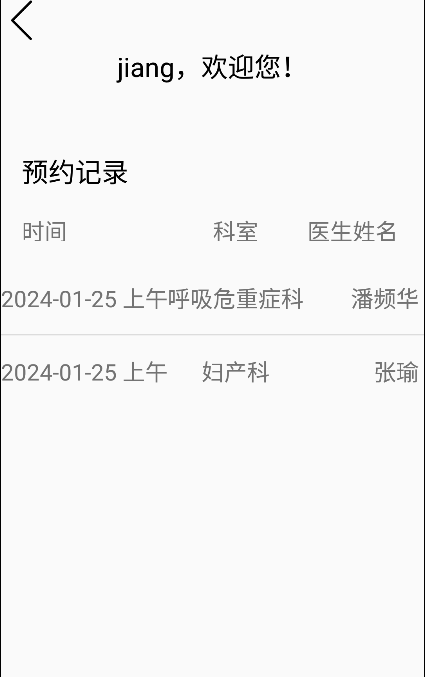
\includegraphics[width=0.3\textwidth]{imgs/26.png}
    \caption{我的信息界面}
\end{figure}

\newpage

\subsection{后台管理系统测试结果}

\subsubsection{登录界面}

\begin{figure}[htbp]
    \centering
    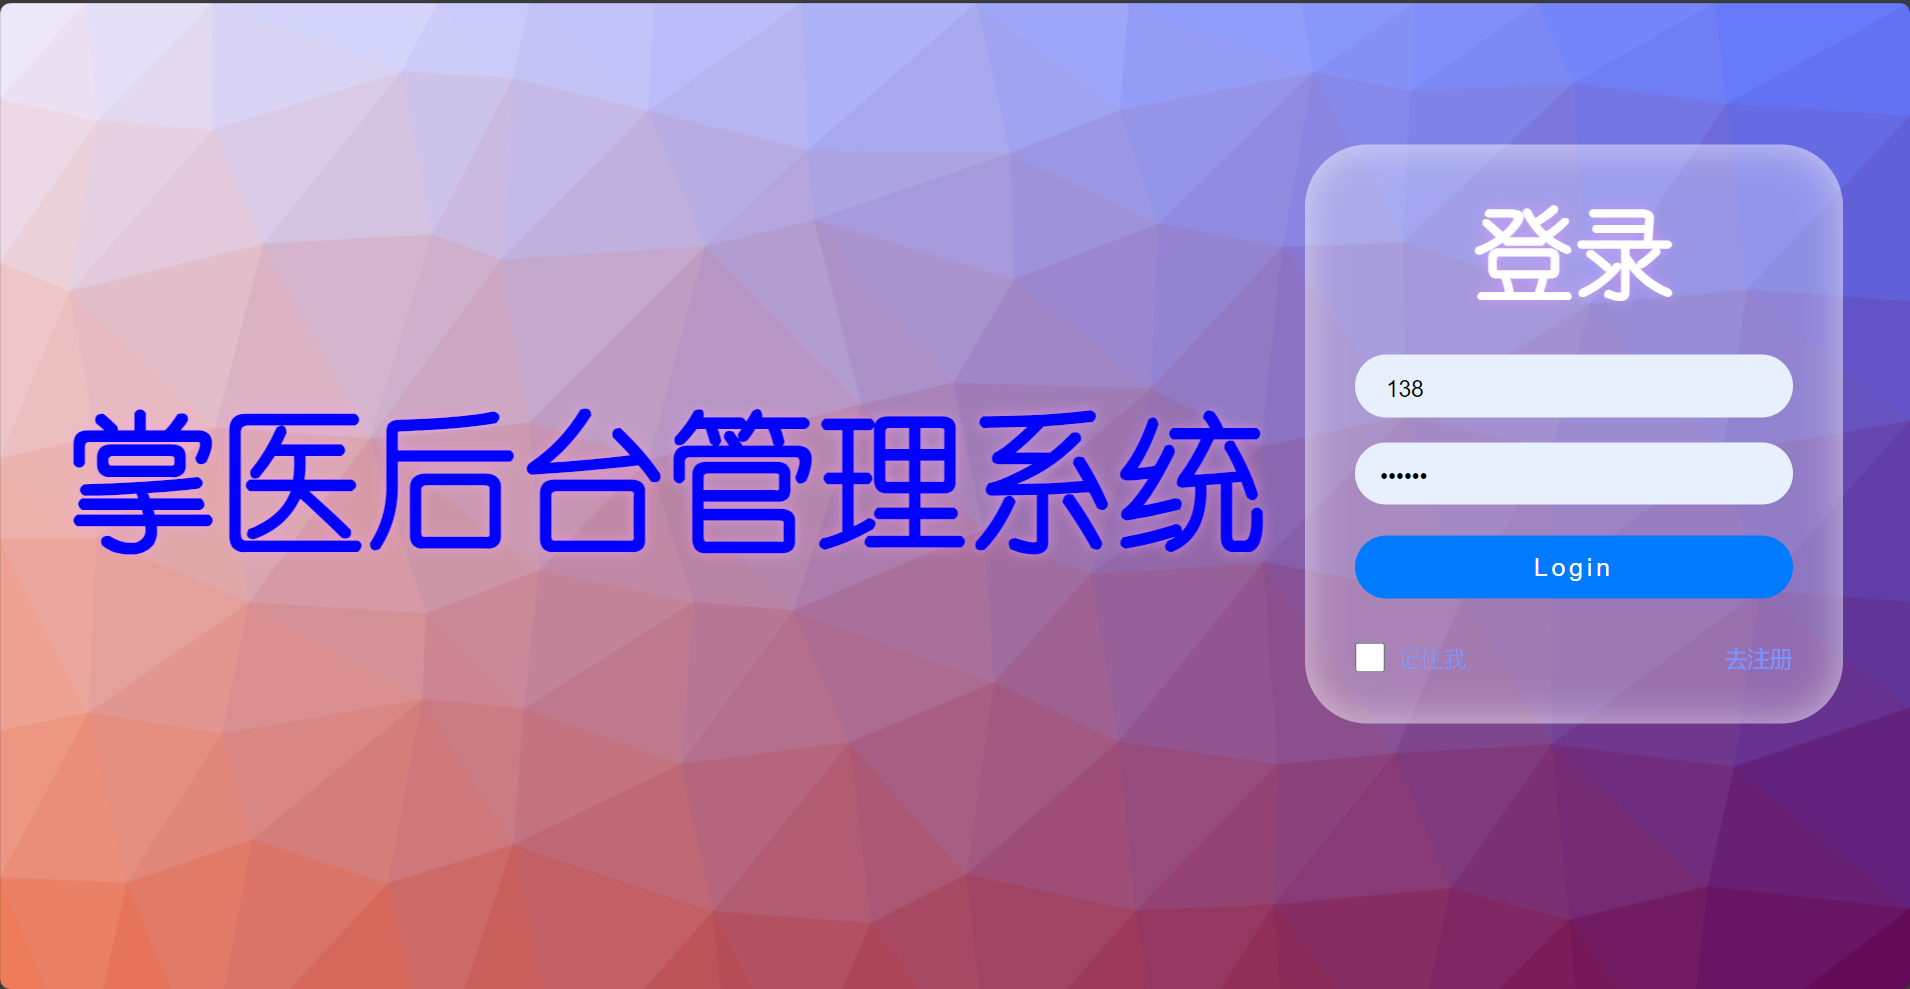
\includegraphics[width=0.8\textwidth]{imgs/33.png}
    \caption{登录界面}
\end{figure}

\subsubsection{控制台界面}

\begin{figure}[htbp]
    \centering
    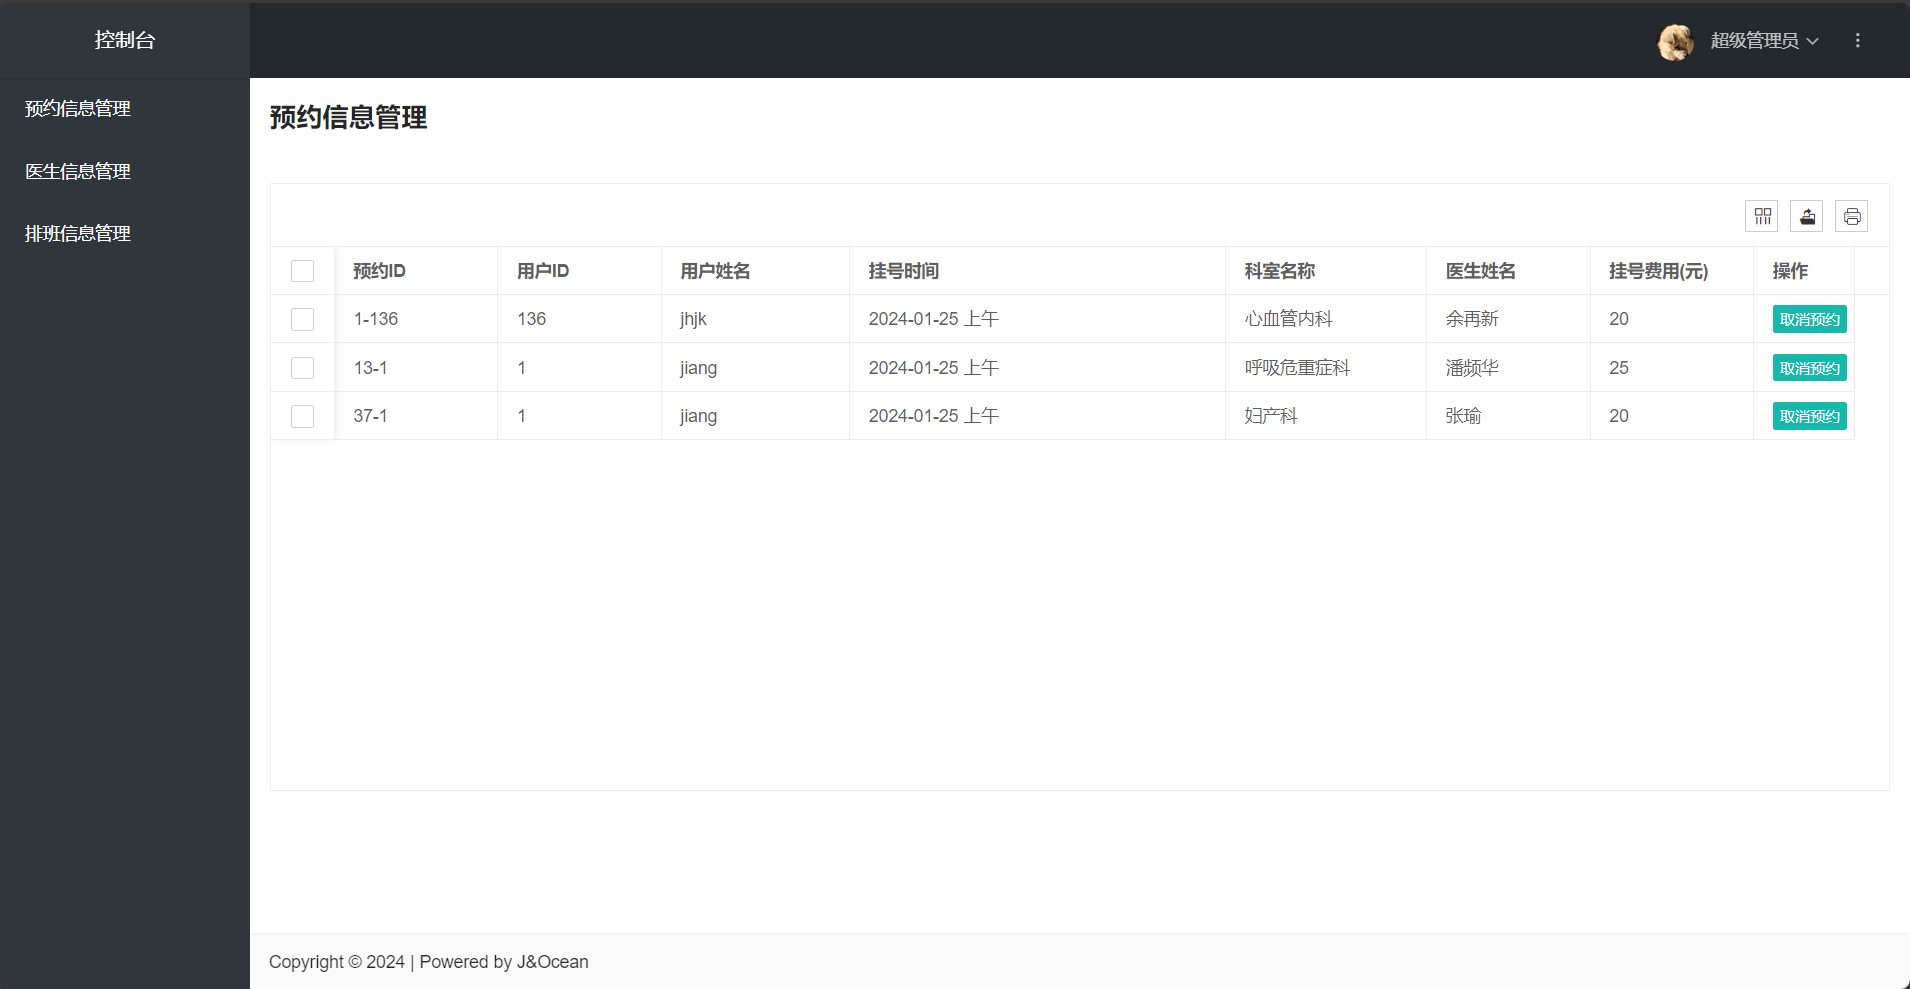
\includegraphics[width=0.8\textwidth]{imgs/34.png}
    \caption{控制台界面}
\end{figure}

\newpage

\subsubsection{预约信息管理界面}
取消预约功能测试结果如下图所示:

\begin{figure}[htbp]
    \centering
    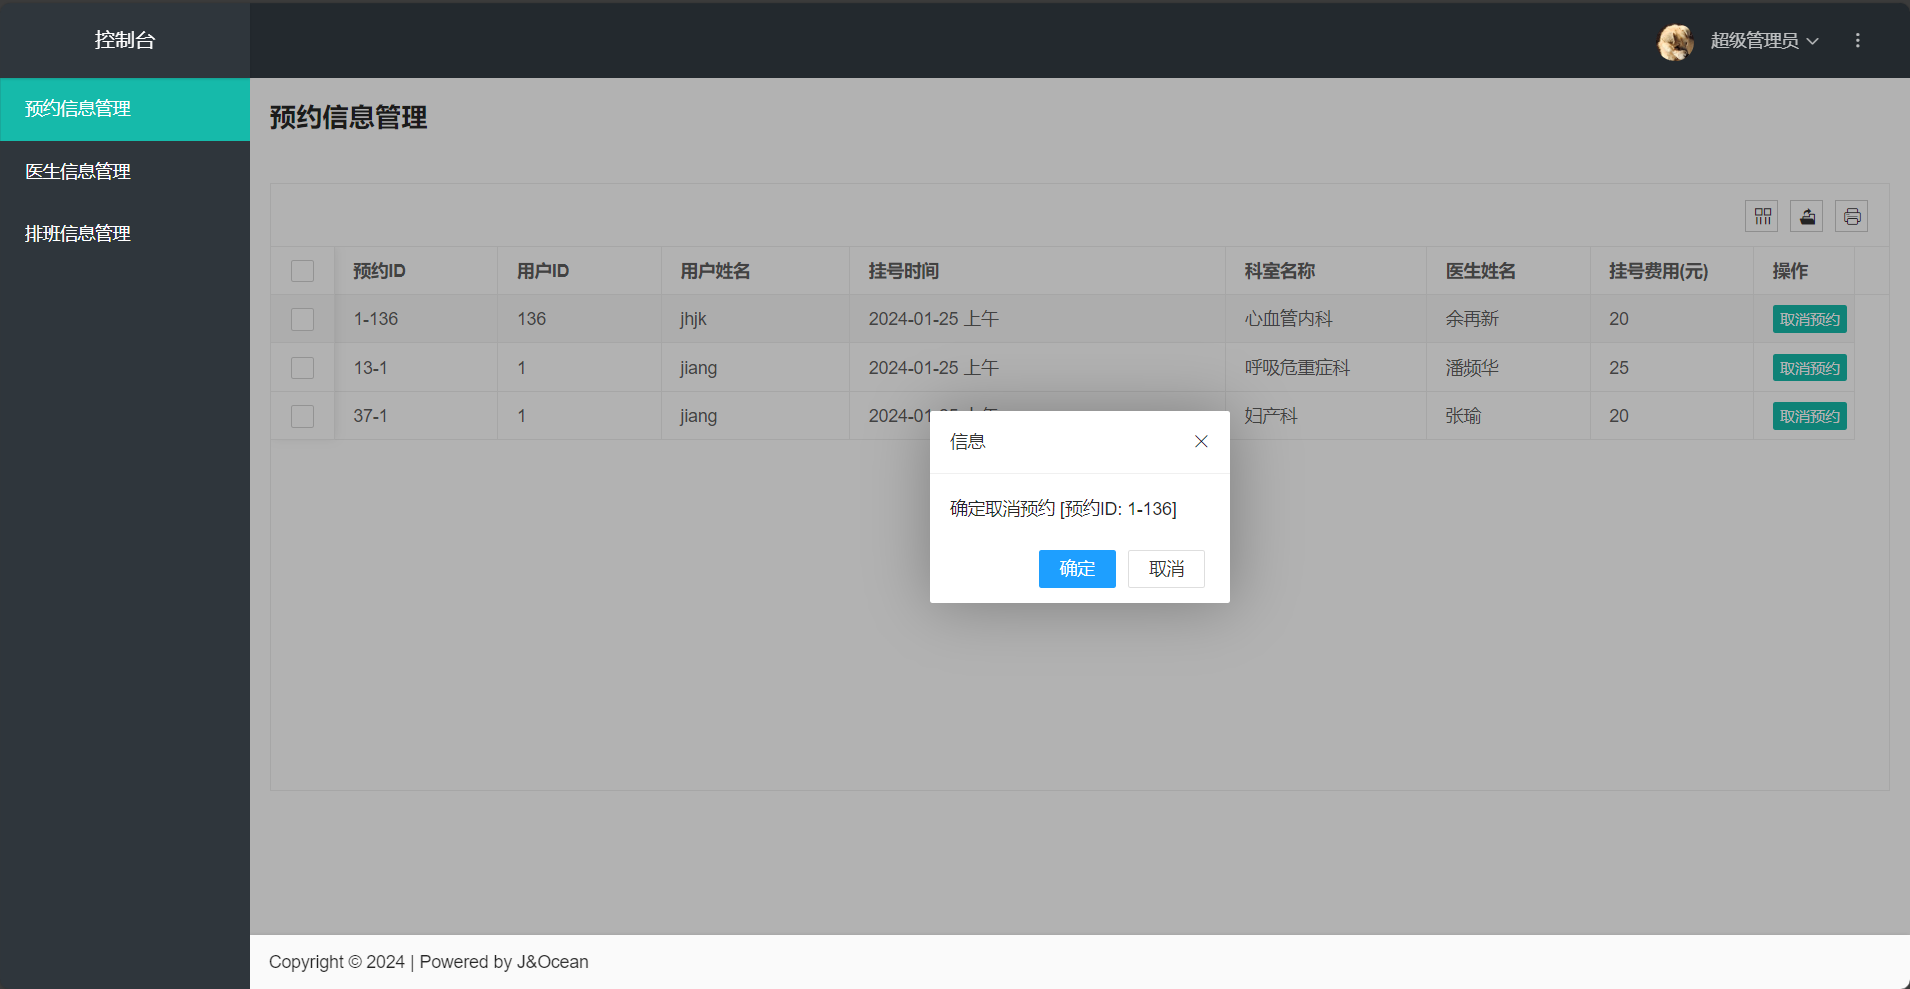
\includegraphics[width=0.8\textwidth]{imgs/35.png}
    \caption{医生信息管理界面}
\end{figure}

\begin{figure}[htbp]
    \centering
    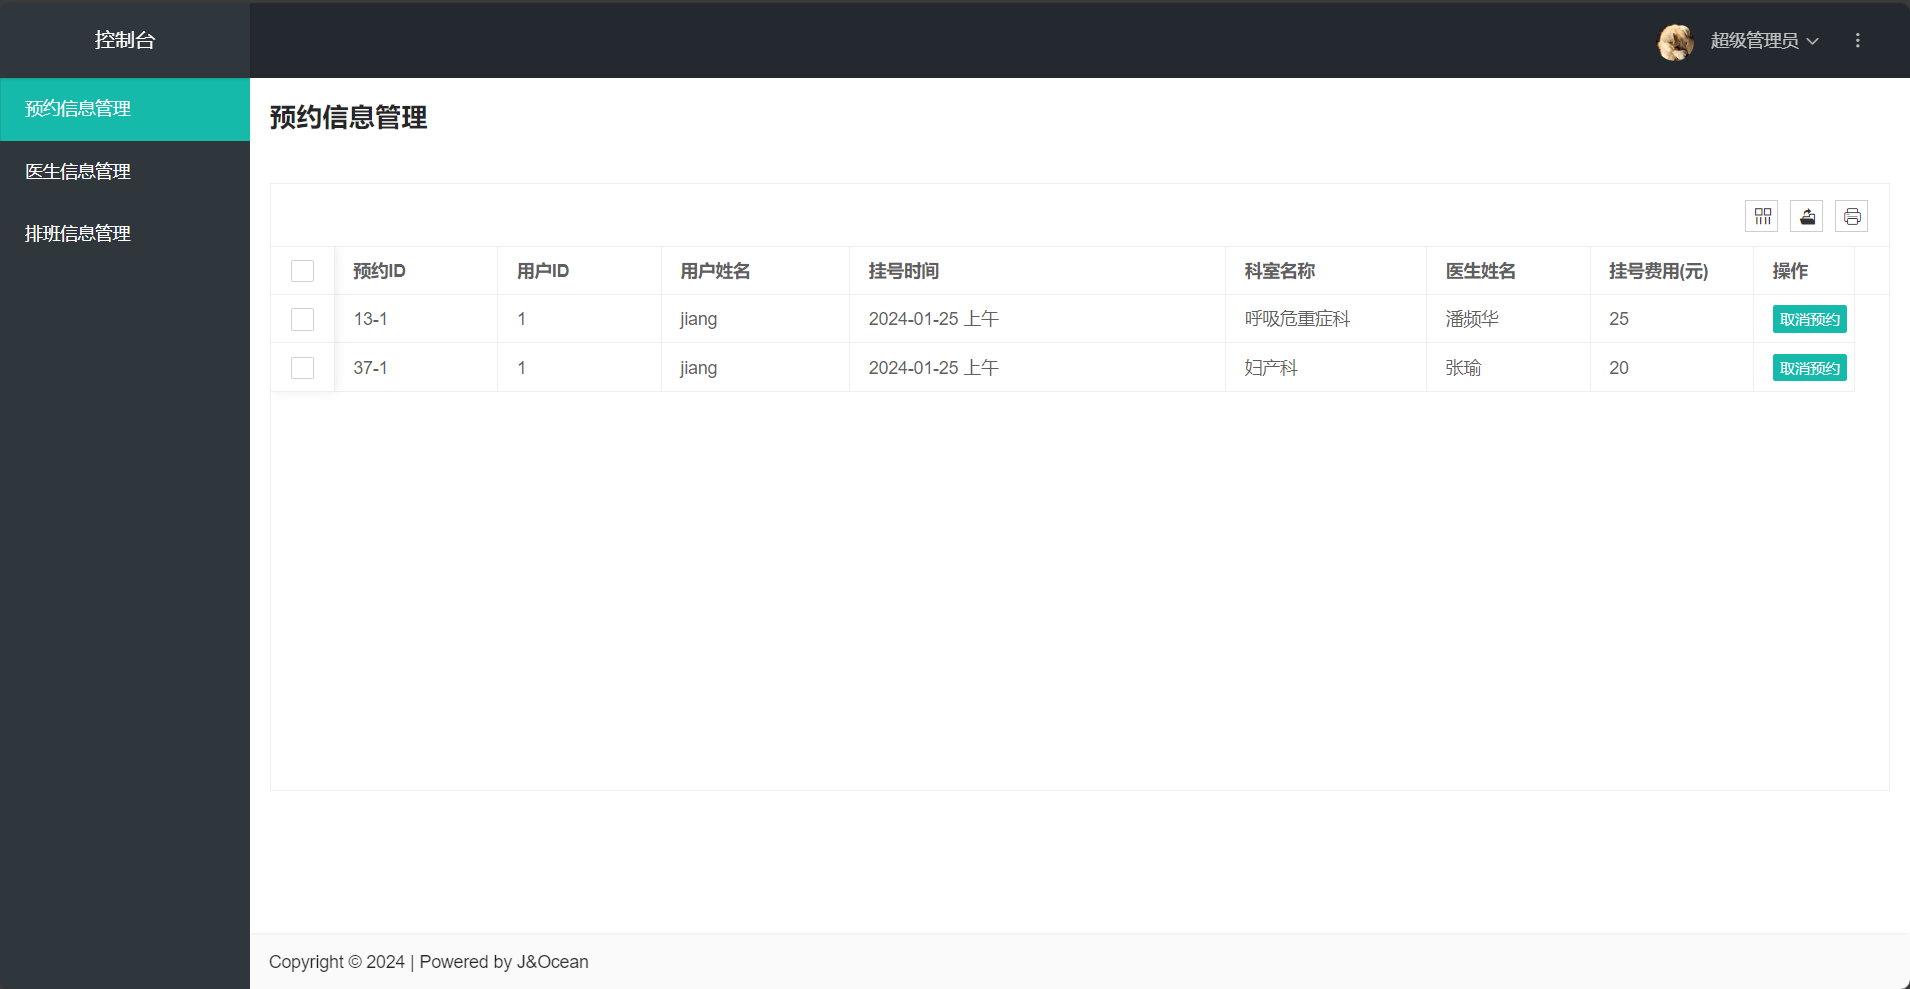
\includegraphics[width=0.8\textwidth]{imgs/36.png}
    \caption{取消预约功能测试结果}
\end{figure}

\newpage

\subsubsection{医生信息管理界面}
修改医生信息功能测试结果如下图所示:

\begin{figure}[htbp]
    \centering
    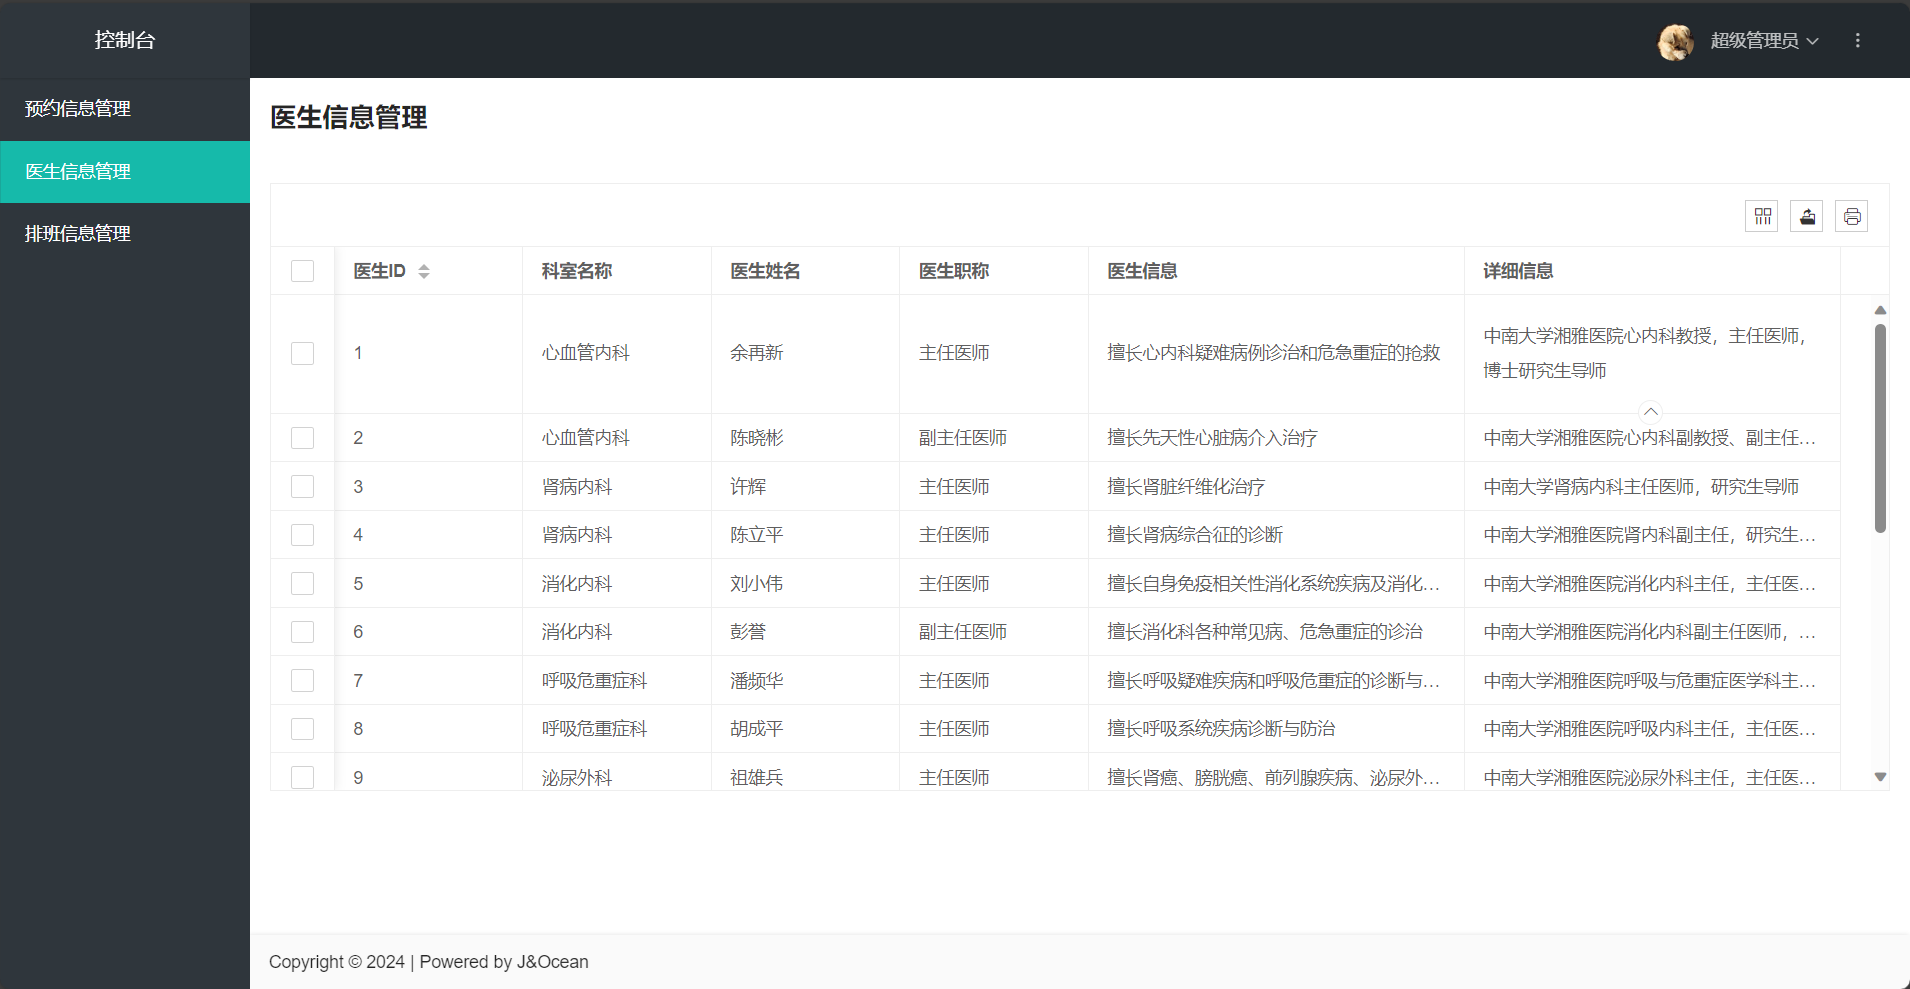
\includegraphics[width=0.8\textwidth]{imgs/37.png}
    \caption{医生信息管理界面}
\end{figure}

\begin{figure}[htbp]
    \centering
    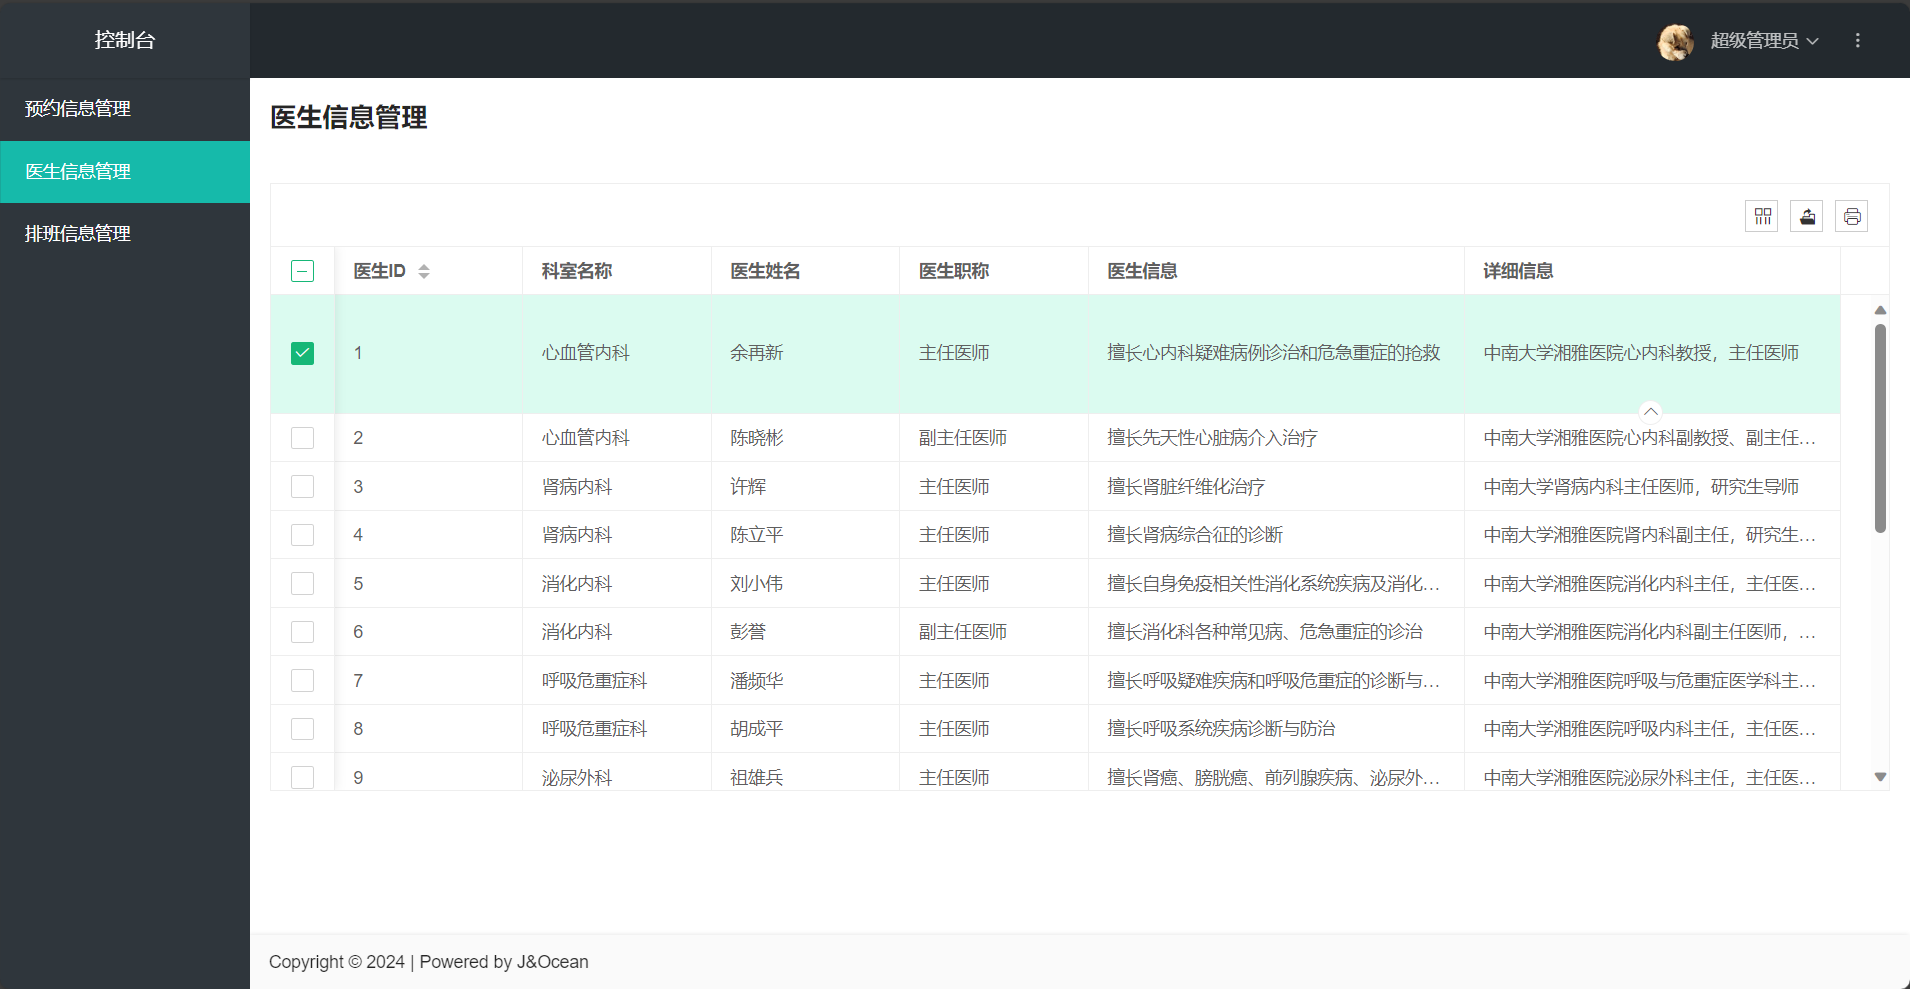
\includegraphics[width=0.8\textwidth]{imgs/38.png}
    \caption{修改医生信息功能测试结果}
\end{figure}

\newpage

\subsubsection{排班信息管理界面}
取消排班功能测试结果如下图所示:

\begin{figure}[htbp]
    \centering
    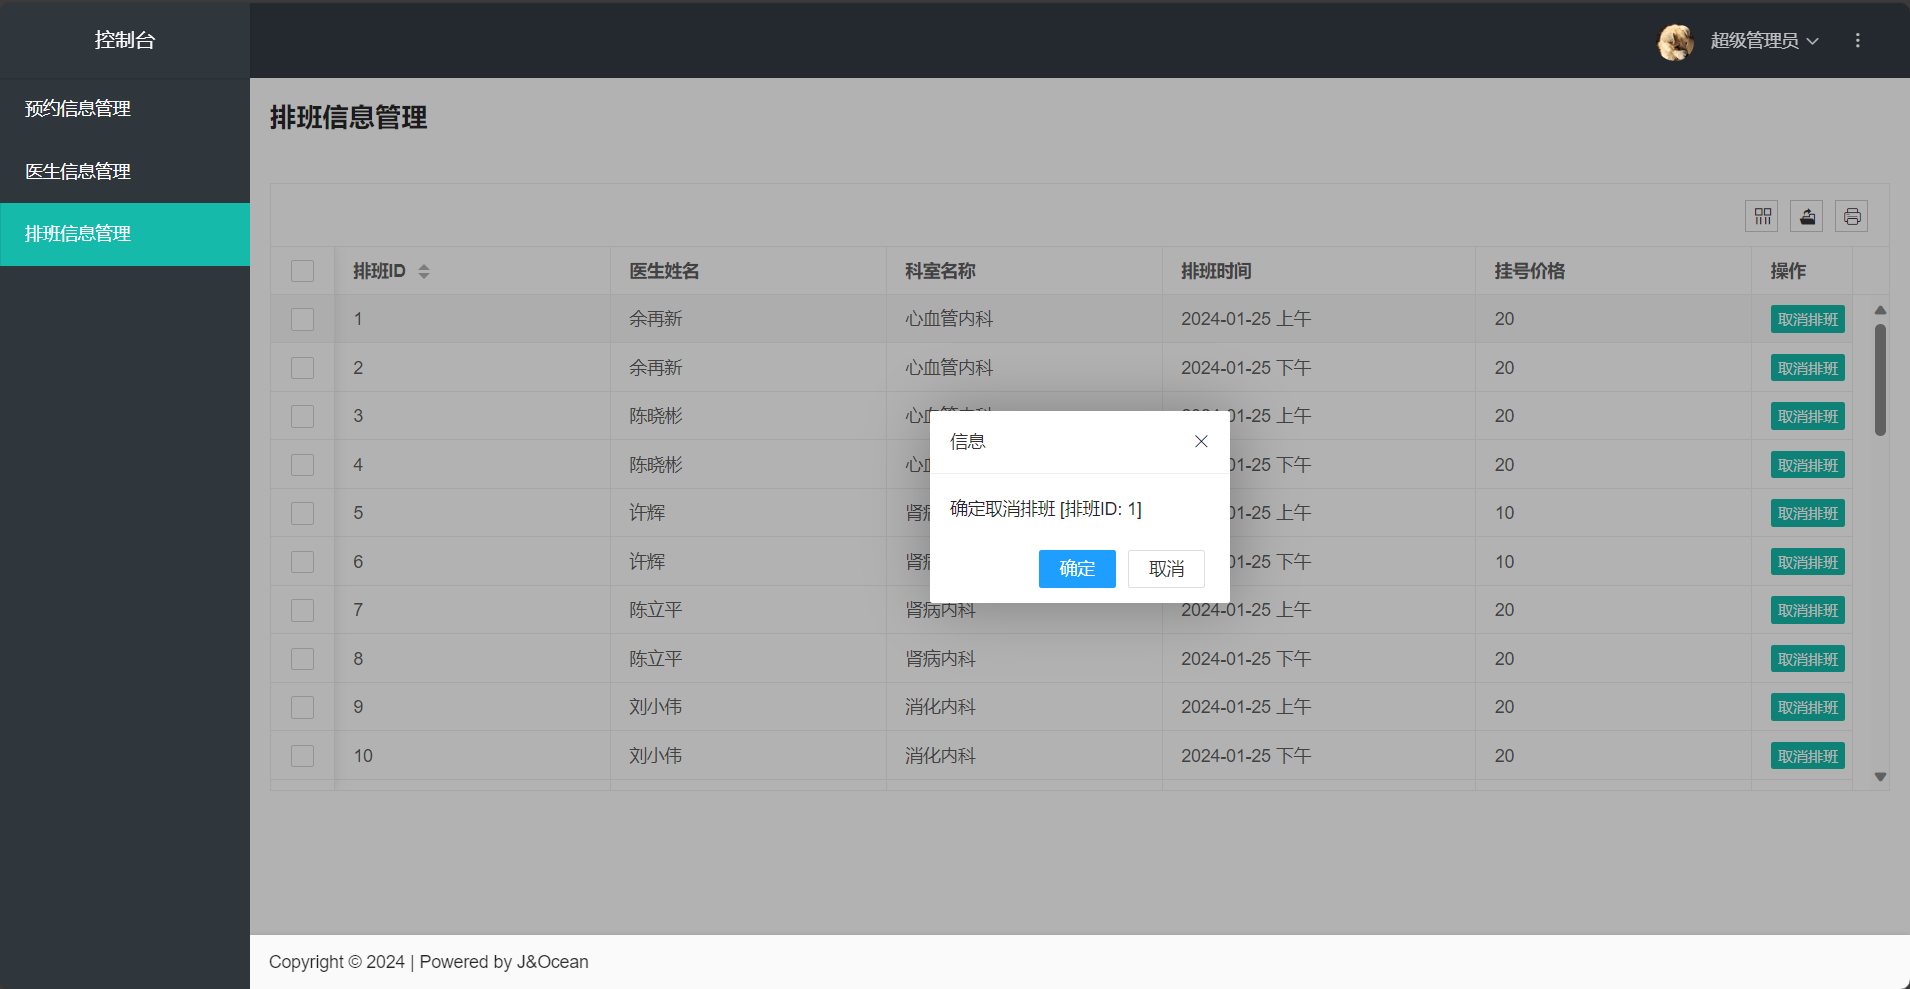
\includegraphics[width=0.8\textwidth]{imgs/39.png}
    \caption{排班信息管理界面}
\end{figure}

\begin{figure}[htbp]
    \centering
    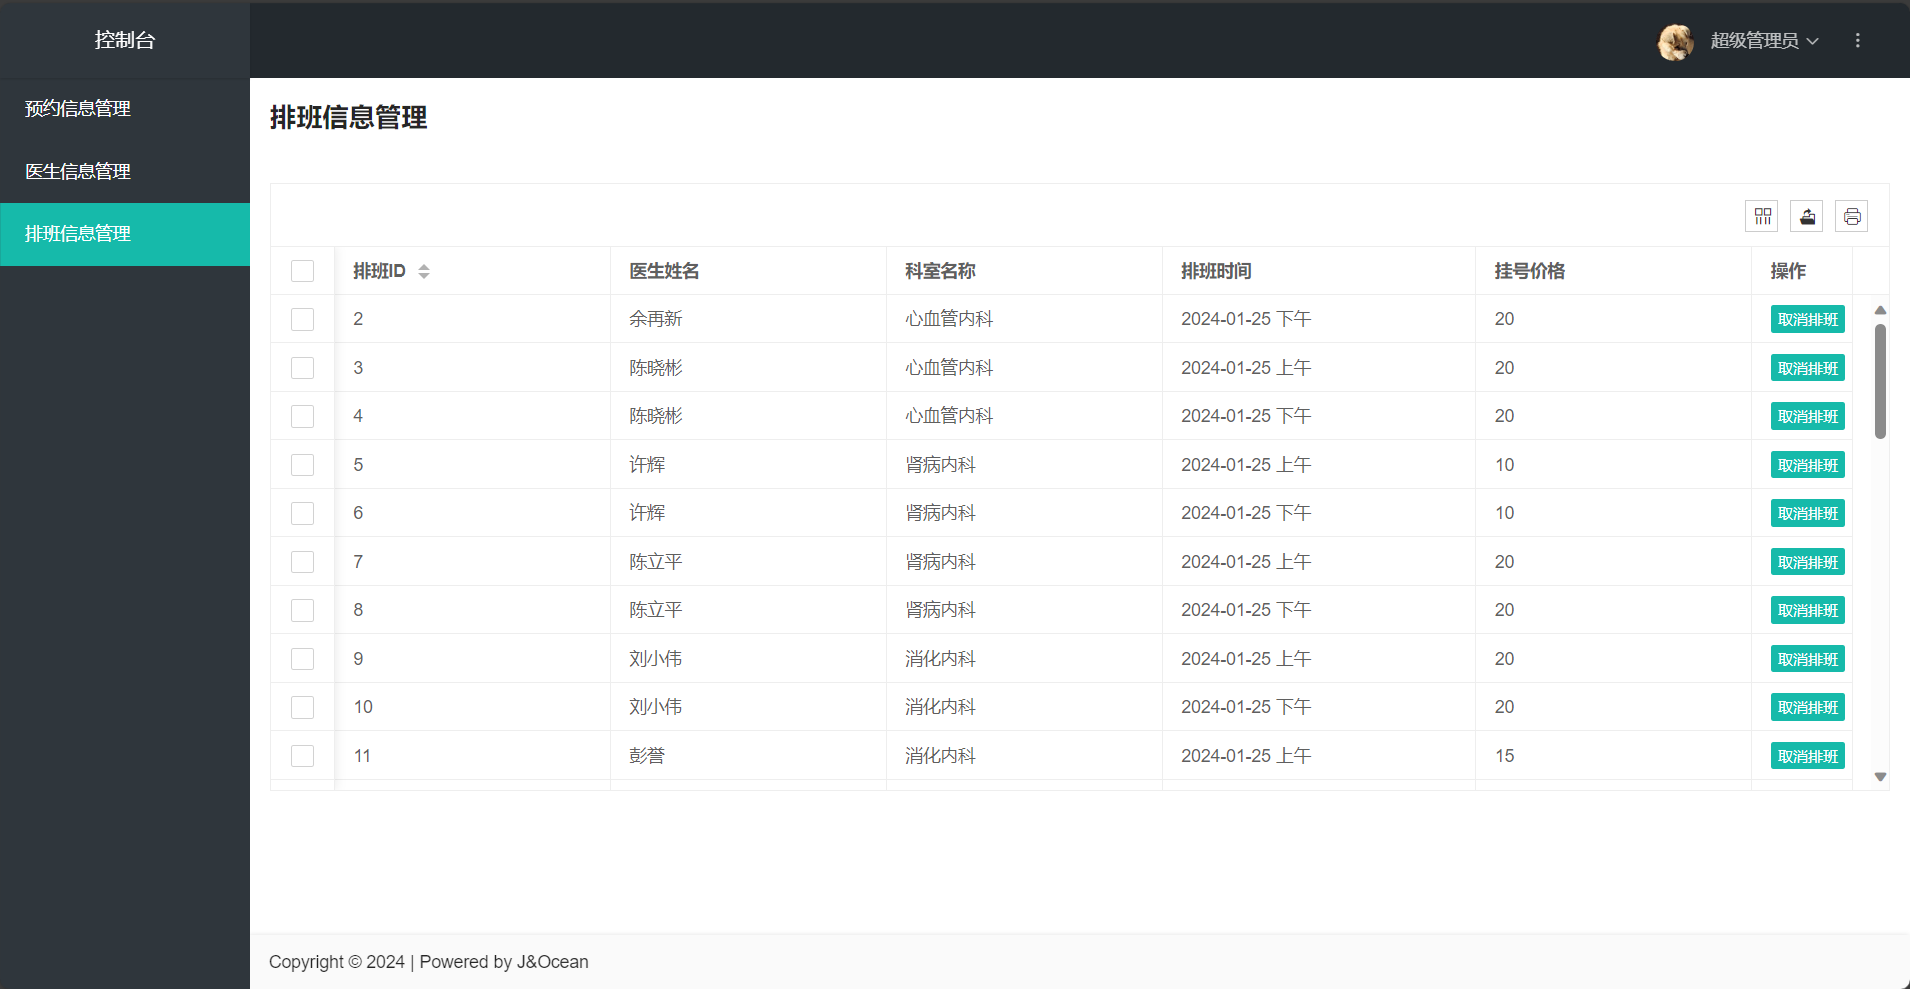
\includegraphics[width=0.8\textwidth]{imgs/40.png}
    \caption{取消排班功能测试结果}
\end{figure}

\newpage

\section{心得体会}

\subsection{熟悉移动端+后台管理系统+服务器的开发流程}
在本次课程设计中,我需要掌握Android移动应用开发+Web Servlet开发+MySQL数据库开发,
其中移动应用开发是我之前没有接触过的,前端Web页面开发自学过一些,但是没有实际开发经验。

本次实战中,发现之前学习的知识并不能完全满足实际开发的需求,因此需要在实战中不断学习,不断查阅资料,不断调试,才能完成本次课程设计。
本次实战中,快速掌握了Android移动应用开发+Web Servlet开发+MySQL数据库开发的开发流程,对于以后的开发有了一定的经验。

\subsection{提升自己的动手能力}
这次实践涉及到不少知识盲区,在这个过程中,查阅书籍、查阅教程、阅读官方文档和博客并学会应用等,克服了很多
困难,也在这个不断学习的过程中锻炼了自己的自学能力。

\subsection{增强系统开发能力}
本学期学习了软件工程这门课程,在面向对象分析、设计中学习到的用例建模等知识在本次课程设计中得到了实践,对于软件开发有了更深的认识,
自顶向下的开发方式,先分析需求,再设计系统,最后实现系统,这样的开发方式,可以提高开发效率,减少开发成本,提高软件质量。

将系统划分为三大模块:移动端、后台管理系统、服务器,然后再将每个模块划分为多个子模块,分别实现,最后再将各个子模块整合到一起,这样的开发方式能够提高开发效率,减少开发成本,提高软件质量。

\subsection{学会调试代码}
在本次课程设计中,Android开发、Web服务器开发的接口输出需要规范,查看输出的过程中,发现输出的格式不符合要求,因此需要调试代码;
调试代码的过程中,发现了很多问题,比如说,Android端连接服务器失败,Android端连接服务器成功,但是无法获取数据,账号密码的传输安全问题,前端动态渲染表格失败等等,通过调试代码,解决了这些问题,提高了自己的调试能力。

\subsection{学会使用前端框架}
在本次课程设计中,使用了layui前端框架,前端框架美化了前端页面,提高了开发效率,减少了开发成本,提高了软件质量,能够让我专注于业务逻辑的实现,而不是花费大量的时间在前端页面的开发上。

\newpage

\section{参考文献}

\begin{enumerate}
    \item Android开发者文档:https://developer.android.google.cn/?hl=zh-cn
    \item Servlet开发者文档:https://www.dba.cn/book/servlet/
    \item Layui文档:https://layui.dev/docs/2/
    \item Bill Phillips Brian Hardy, Android 编程权威指南(第三版) [M],北京,人民邮电出版社2017
\end{enumerate}

\newpage

\section{附录}
\subsection{Android端代码清单}
\subsubsection{java}
\begin{itemize}
    \item com.example.palmhospital.bean
    \begin{itemize}
        \item Depart.java
        \item Doctor.java
        \item Order.java
        \item Schedule.java
        \item User.java
    \end{itemize}
    \item com.example.palmhospital.ui.activity
    \begin{itemize}
        \item ChooseDepartActivity.java
        \item ChooseDoctorActivity.java
        \item ChooseTimeActivity.java
        \item DoctorDetailActivity.java
        \item IndexActivity.java
        \item LoginActivity.java
        \item MyInfoActivity.java
        \item PayActivity.java
        \item RegisterActivity.java
        \item SplashActivity.java
    \end{itemize}
    \item com.example.palmhospital.utils
    \begin{itemize}
        \item NetUtil.java
    \end{itemize}
    \item Config.java
\end{itemize}
\subsubsection{res}
主要列举layout的文件清单
\begin{itemize}
    \item activity\_choose\_depart.xml
    \item activity\_choose\_doctor.xml
    \item activity\_choose\_time.xml
    \item activity\_doctor\_detail.xml
    \item activity\_index.xml
    \item activity\_login.xml
    \item activity\_my\_info.xml
    \item activity\_pay.xml
    \item activity\_register.xml
    \item activity\_splash.xml
    \item item\_depart\_list\_view.xml
    \item item\_doctor\_list\_view.xml
    \item item\_myinfo\_list\_view.xml
    \item item\_time\_list\_view.xml
\end{itemize}

\subsubsection{AndroidManifest.xml}
AndroidManifest.xml文件是整个应用程序的信息描述文件,定义了应用程序中包含的Activity,Service,Content provider和BroadcastReceiver组件信息。

\begin{lstlisting}[frame=shadowbox]
    <?xml version="1.0" encoding="utf-8"?>
<manifest xmlns:android="http://schemas.android.com/apk/res/android"
    package="com.example.palmhospital">

    <uses-permission android:name="android.permission.INTERNET" />
    <uses-permission android:name="android.permission.ACCESS_NETWORK_STATE" />
    <uses-permission android:name="android.permission.ACCESS_WIFI_STATE" />

    <application
        android:allowBackup="true"
        android:icon="@mipmap/icon_zhangyi"
        android:label="@string/app_name"
        android:networkSecurityConfig="@xml/network_security_config"
        android:roundIcon="@mipmap/icon_zhangyi"
        android:supportsRtl="true"
        android:theme="@style/Theme.PalmHospital">
        <activity
            android:name=".ui.activity.PayActivity"
            android:exported="true" />
        <activity
            android:name=".ui.activity.DoctorDetailActivity"
            android:exported="true" />
        <activity
            android:name=".ui.activity.ChooseTimeActivity"
            android:exported="true" />
        <activity
            android:name=".ui.activity.MyInfoActivity"
            android:exported="true" />
        <activity
            android:name=".ui.activity.ChooseDoctorActivity"
            android:exported="true" />
        <activity
            android:name=".ui.activity.ChooseDepartActivity"
            android:exported="true" />
        <activity
            android:name=".ui.activity.IndexActivity"
            android:exported="true" />


        <activity
            android:name=".ui.activity.RegisterActivity"
            android:exported="true" />
        <activity
            android:name=".ui.activity.LoginActivity"
            android:exported="true" />
        <activity
            android:name=".ui.activity.SplashActivity"
            android:exported="true">
            <intent-filter>
                <action android:name="android.intent.action.MAIN" />

                <category android:name="android.intent.category.LAUNCHER" />
            </intent-filter>
        </activity>
    </application>

</manifest>
\end{lstlisting}

\subsection{后台管理系统及服务器代码清单}
\subsubsection{java}
\begin{itemize}
    \item com.example.palmhospitalservice.backend
    \begin{itemize}
        \item BackRegisterServlet.java
        \item DeleteOrdersServlet.java
        \item DeleteSchedulesServlet.java
        \item DoctorServlet.java
        \item LogoutServlet.java
        \item OrderServlet.java
        \item ScheduleServlet.java
        \item TestServlet.java
    \end{itemize}
    \item com.example.palmhospitalservice.bean
    \begin{itemize}
        \item Administrator.java
        \item BackDoctors.java
        \item BackOrders.java
        \item BackSchedules.java
        \item Depart.java
        \item Doctor.java
        \item Order.java
        \item Schedule.java
        \item User.java
    \end{itemize}
    \item com.example.palmhospitalservice.dao
    \begin{itemize}
        \item AdministratorDao.java
        \item BackDoctorsDao.java
        \item BackOrderDao.java
        \item BackSchedulesDao.java
        \item DepartDao.java
        \item DoctorDao.java
        \item OrderDao.java
        \item ScheduleDao.java
        \item UserDao.java
    \end{itemize}
    \item com.example.palmhospitalservice.servlet
    \begin{itemize}
        \item ChooseDepartServlet.java
        \item ChooseDoctorServlet.java
        \item ChooseTimeServlet.java
        \item LoginServlet.java
        \item MyInfoServlet.java
        \item PayServlet.java
        \item RegisterServlet.java
    \end{itemize}
    \item com.example.palmhospitalservice.utils
    \begin{itemize}
        \item Dbutils.java
    \end{itemize}
\end{itemize}
\subsubsection{resources}
\begin{itemize}
    \item database.properties
\end{itemize}

\subsubsection{webapp}
\begin{itemize}
    \item res 
    \item WEB-INF/lib
    \item controller.jsp
    \item doctors.jsp
    \item login.jsp
    \item orders.jsp
    \item register.jsp
    \item schedules.jsp
\end{itemize}

\newpage


\end{document}